\chapter{Software Design Description}

\section{System Design}

\subsection{System Architecture}

The system is designed as a web-based platform based on a layered client--server architecture. The frontend provides interactive interfaces for students, counselors, mentors, and administrators, while the backend exposes RESTful APIs, implements business logic, integrates external services, and manages persistent data. LLM APIs, the GitHub API, Google OAuth, and job portal crawlers are integrated to personalize recommendations and enrich career information.

\begin{figure}[H]
    \centering
    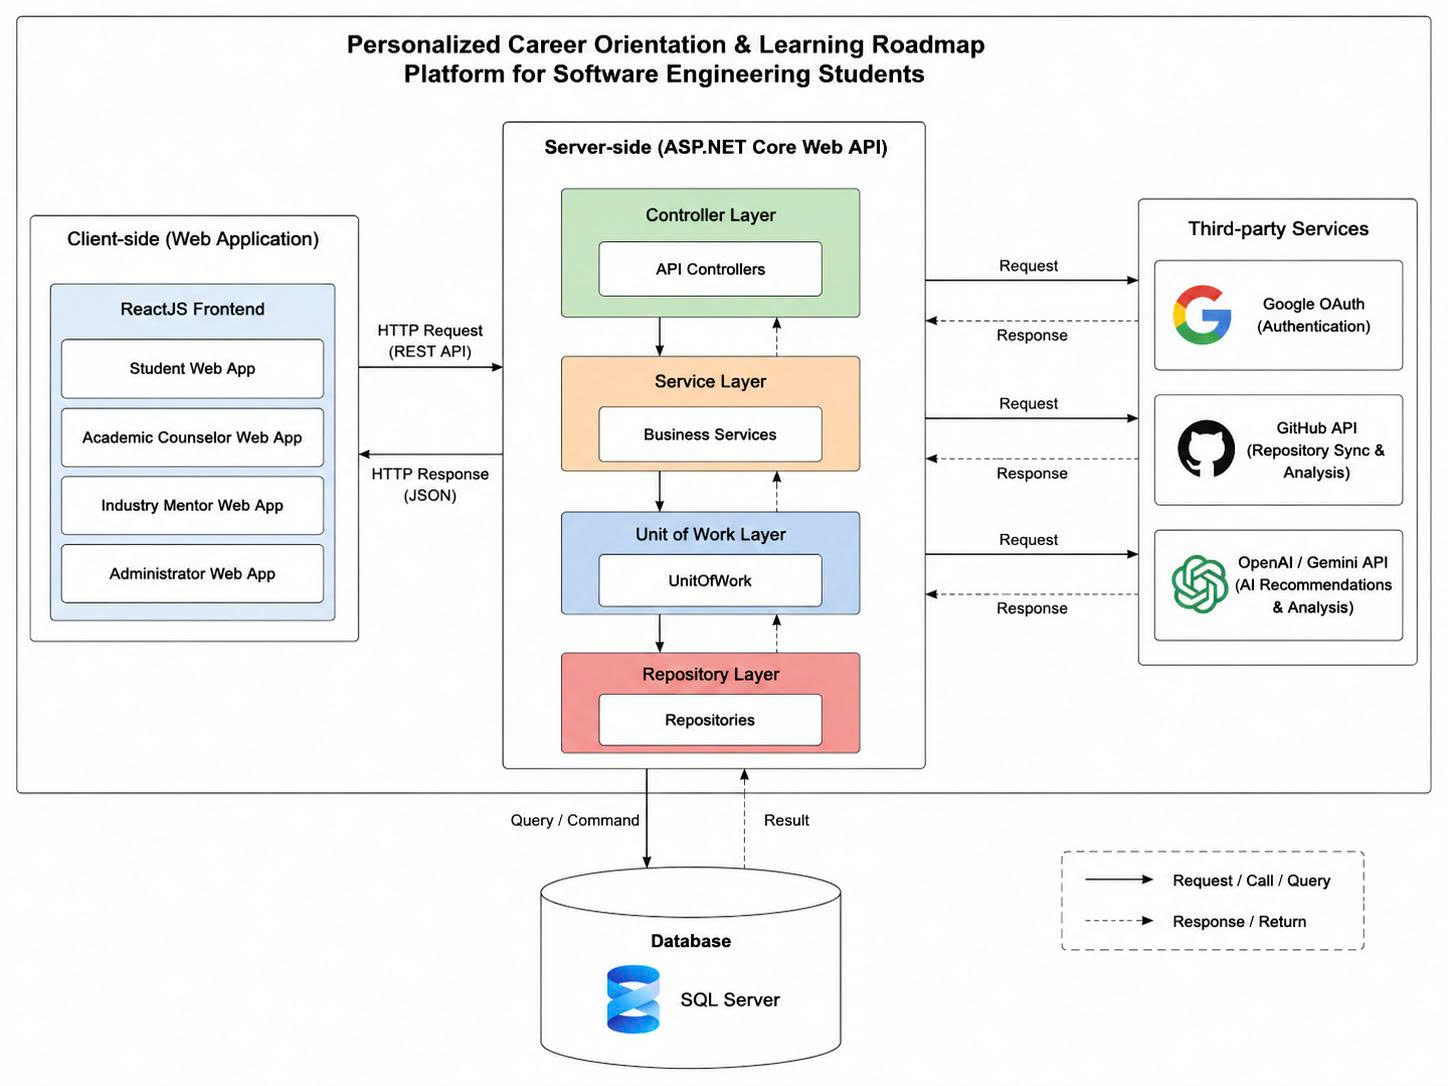
\includegraphics[width=0.95\textwidth]{images/system.jpg}
    \caption{System Architecture Diagram}
    \label{fig:system_architecture}
\end{figure}

\subsubsection{Frontend}

The frontend layer presents information, collects user input, displays roadmap progress, and visualizes skill gap and market trend reports.

\begin{itemize}
    \item \textbf{ReactJS:} Builds a component-based single-page application with reusable user interface modules.
    \item \textbf{TypeScript:} Provides static typing to reduce runtime errors and improve maintainability in complex user interfaces.
    \item \textbf{TailwindCSS:} Supports responsive and consistent styling for dashboards, roadmap trees, cards, forms, and charts.
    \item \textbf{Chart Library:} Visualizes skill gap charts, learning progress statistics, and technology trend graphs.
    \item \textbf{Axios or Fetch API:} Communicates with backend REST APIs for authentication, profile management, roadmap data, AI chat messages, and portfolio information.
\end{itemize}

\begin{figure}[H]
    \centering
    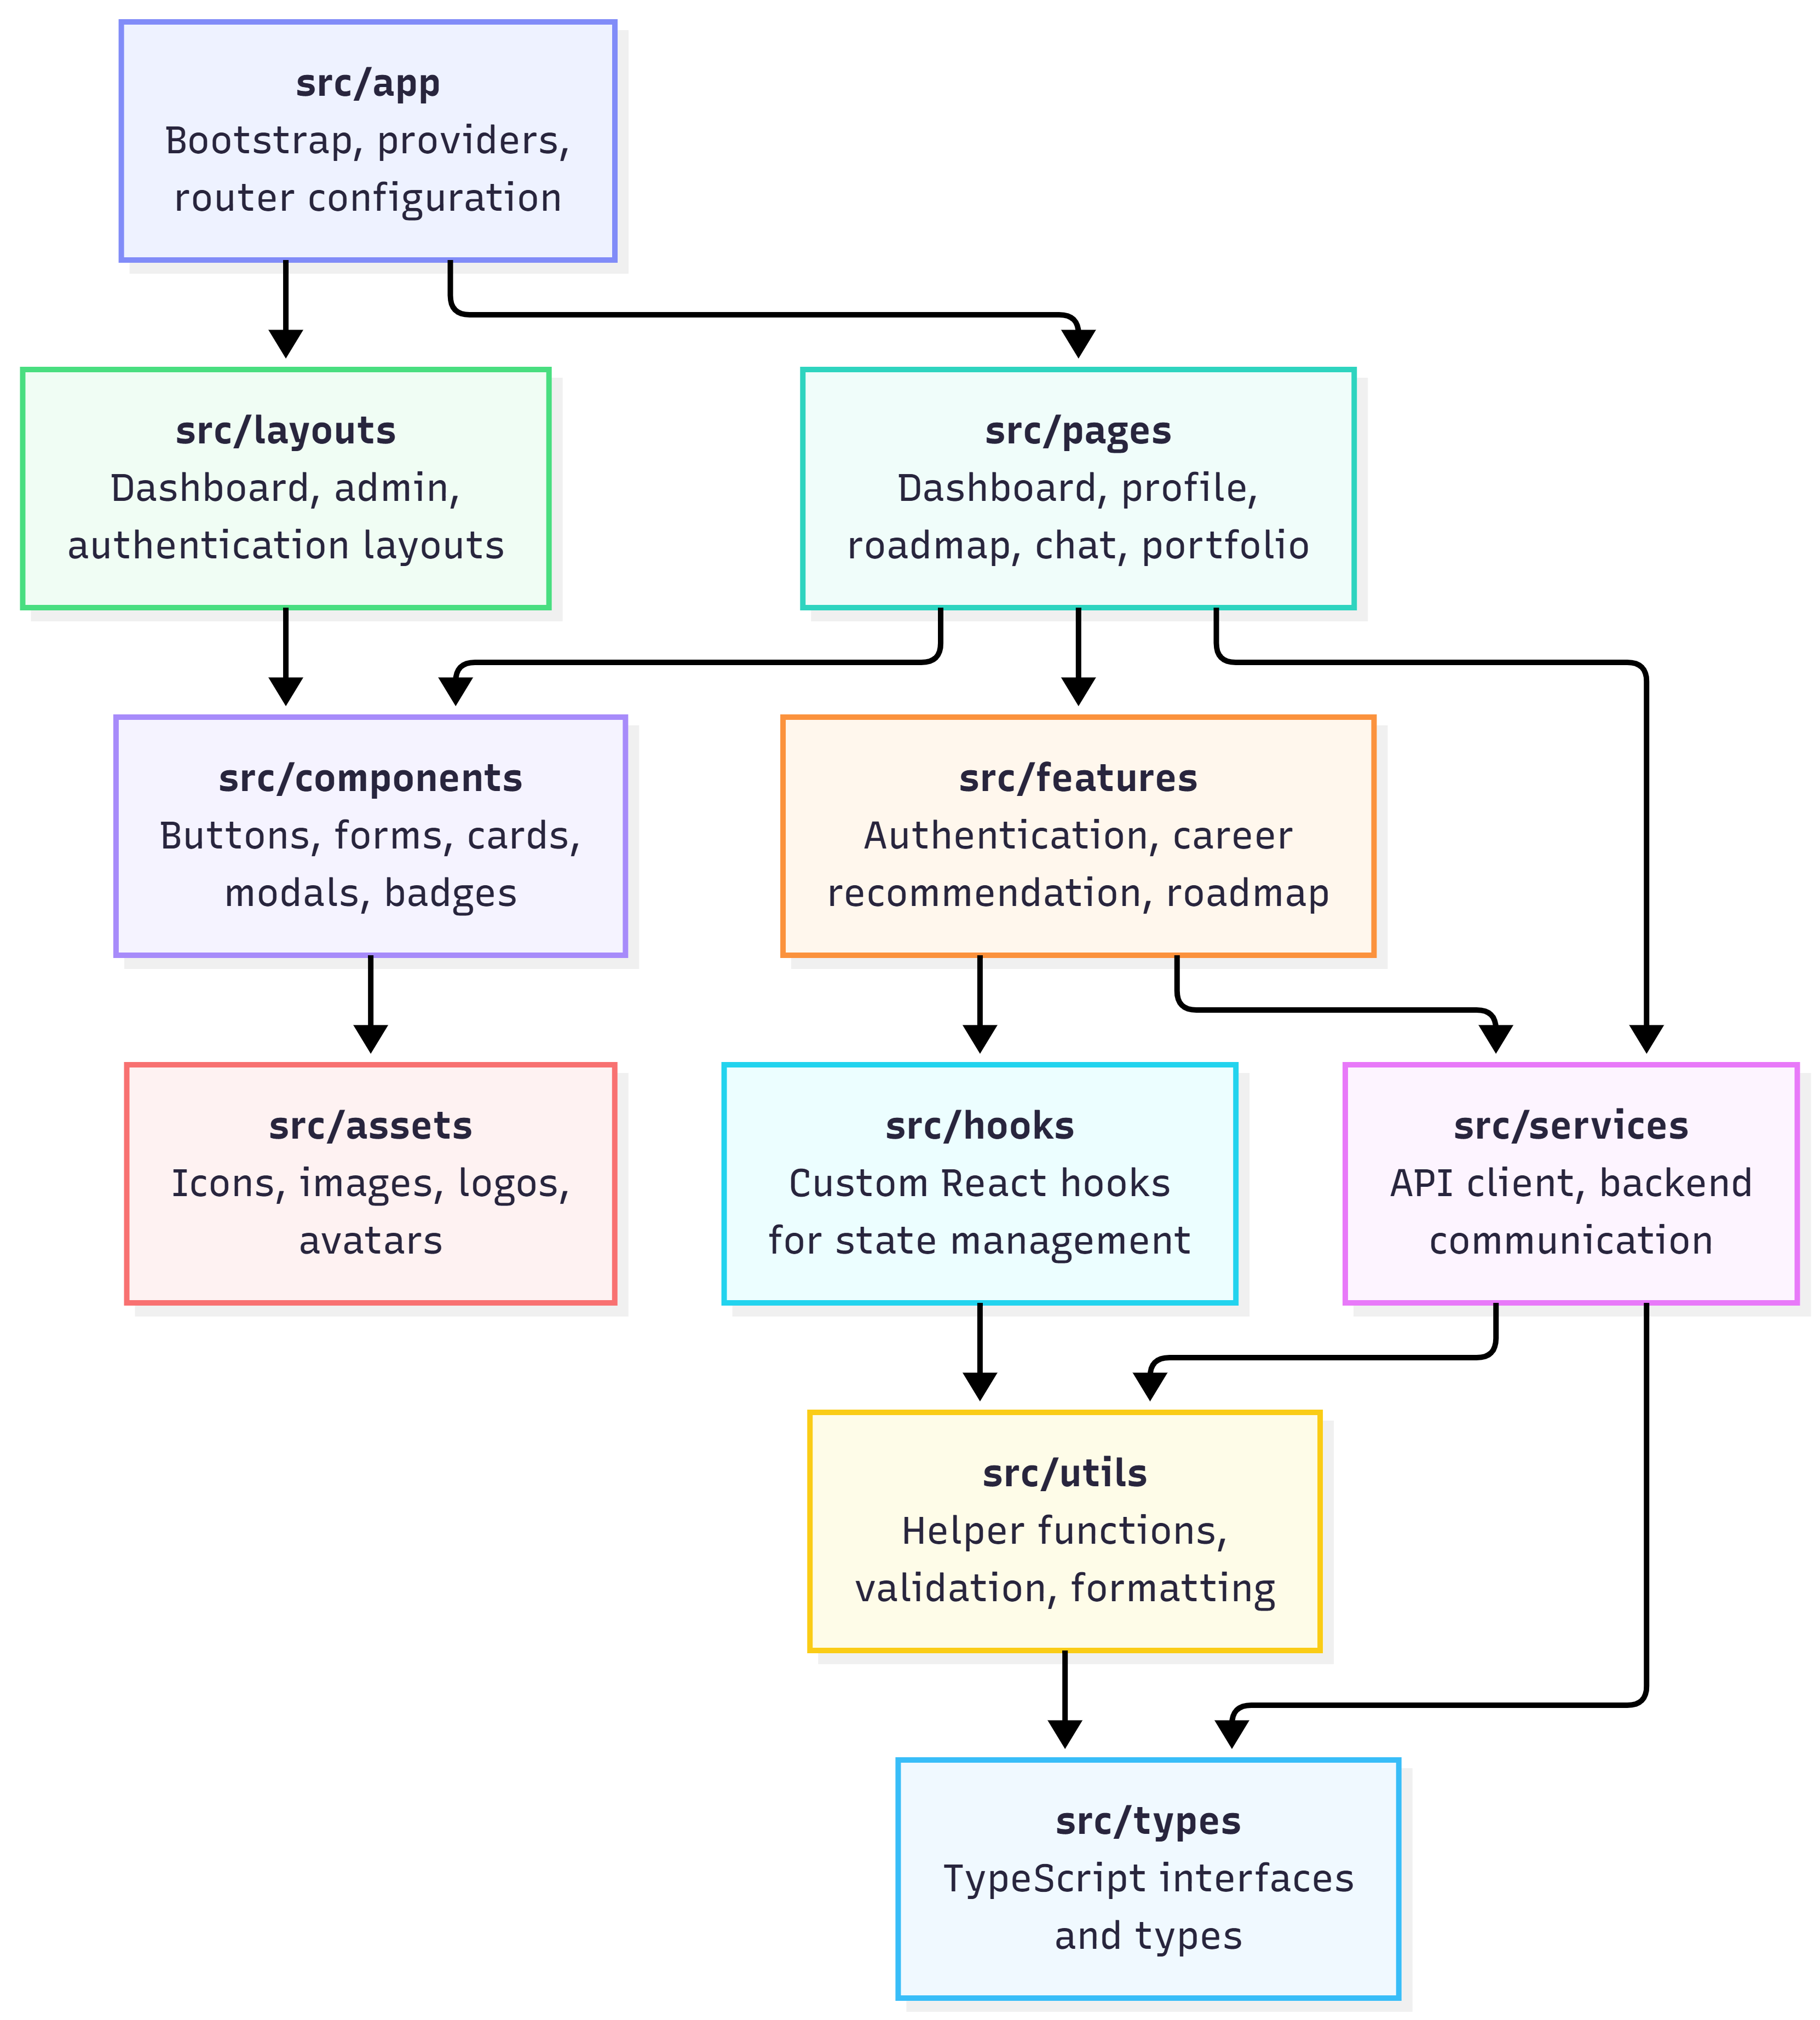
\includegraphics[width=0.95\textwidth]{images/frontend.png}
    \caption{Frontend Architecture Diagram}
    \label{fig:frontend_architecture}
\end{figure}

\subsubsection{Backend}

The backend layer processes the core business logic and coordinates data flow among the frontend, database, AI services, GitHub, and job market data sources.

\begin{itemize}
    \item \textbf{Spring Boot:} Serves as the main backend framework for RESTful APIs, service classes, dependency injection, validation, and security configuration.
    \item \textbf{Spring Security and JWT:} Protects API endpoints, manages login sessions, and supports role-based access control for students, counselors, mentors, and administrators.
    \item \textbf{MySQL:} Stores accounts, student profiles, skill nodes, roadmaps, progress records, mentor sessions, job trends, and portfolio records.
    \item \textbf{JPA/Hibernate:} Maps Java domain entities to database tables and simplifies CRUD operations.
    \item \textbf{Scheduler Service:} Executes daily jobs for collecting labor market data and updating technology trend statistics.
    \item \textbf{File Processing Service:} Handles transcript and CV uploads, extracts important information, and stores file metadata securely.
\end{itemize}

\begin{figure}[H]
    \centering
    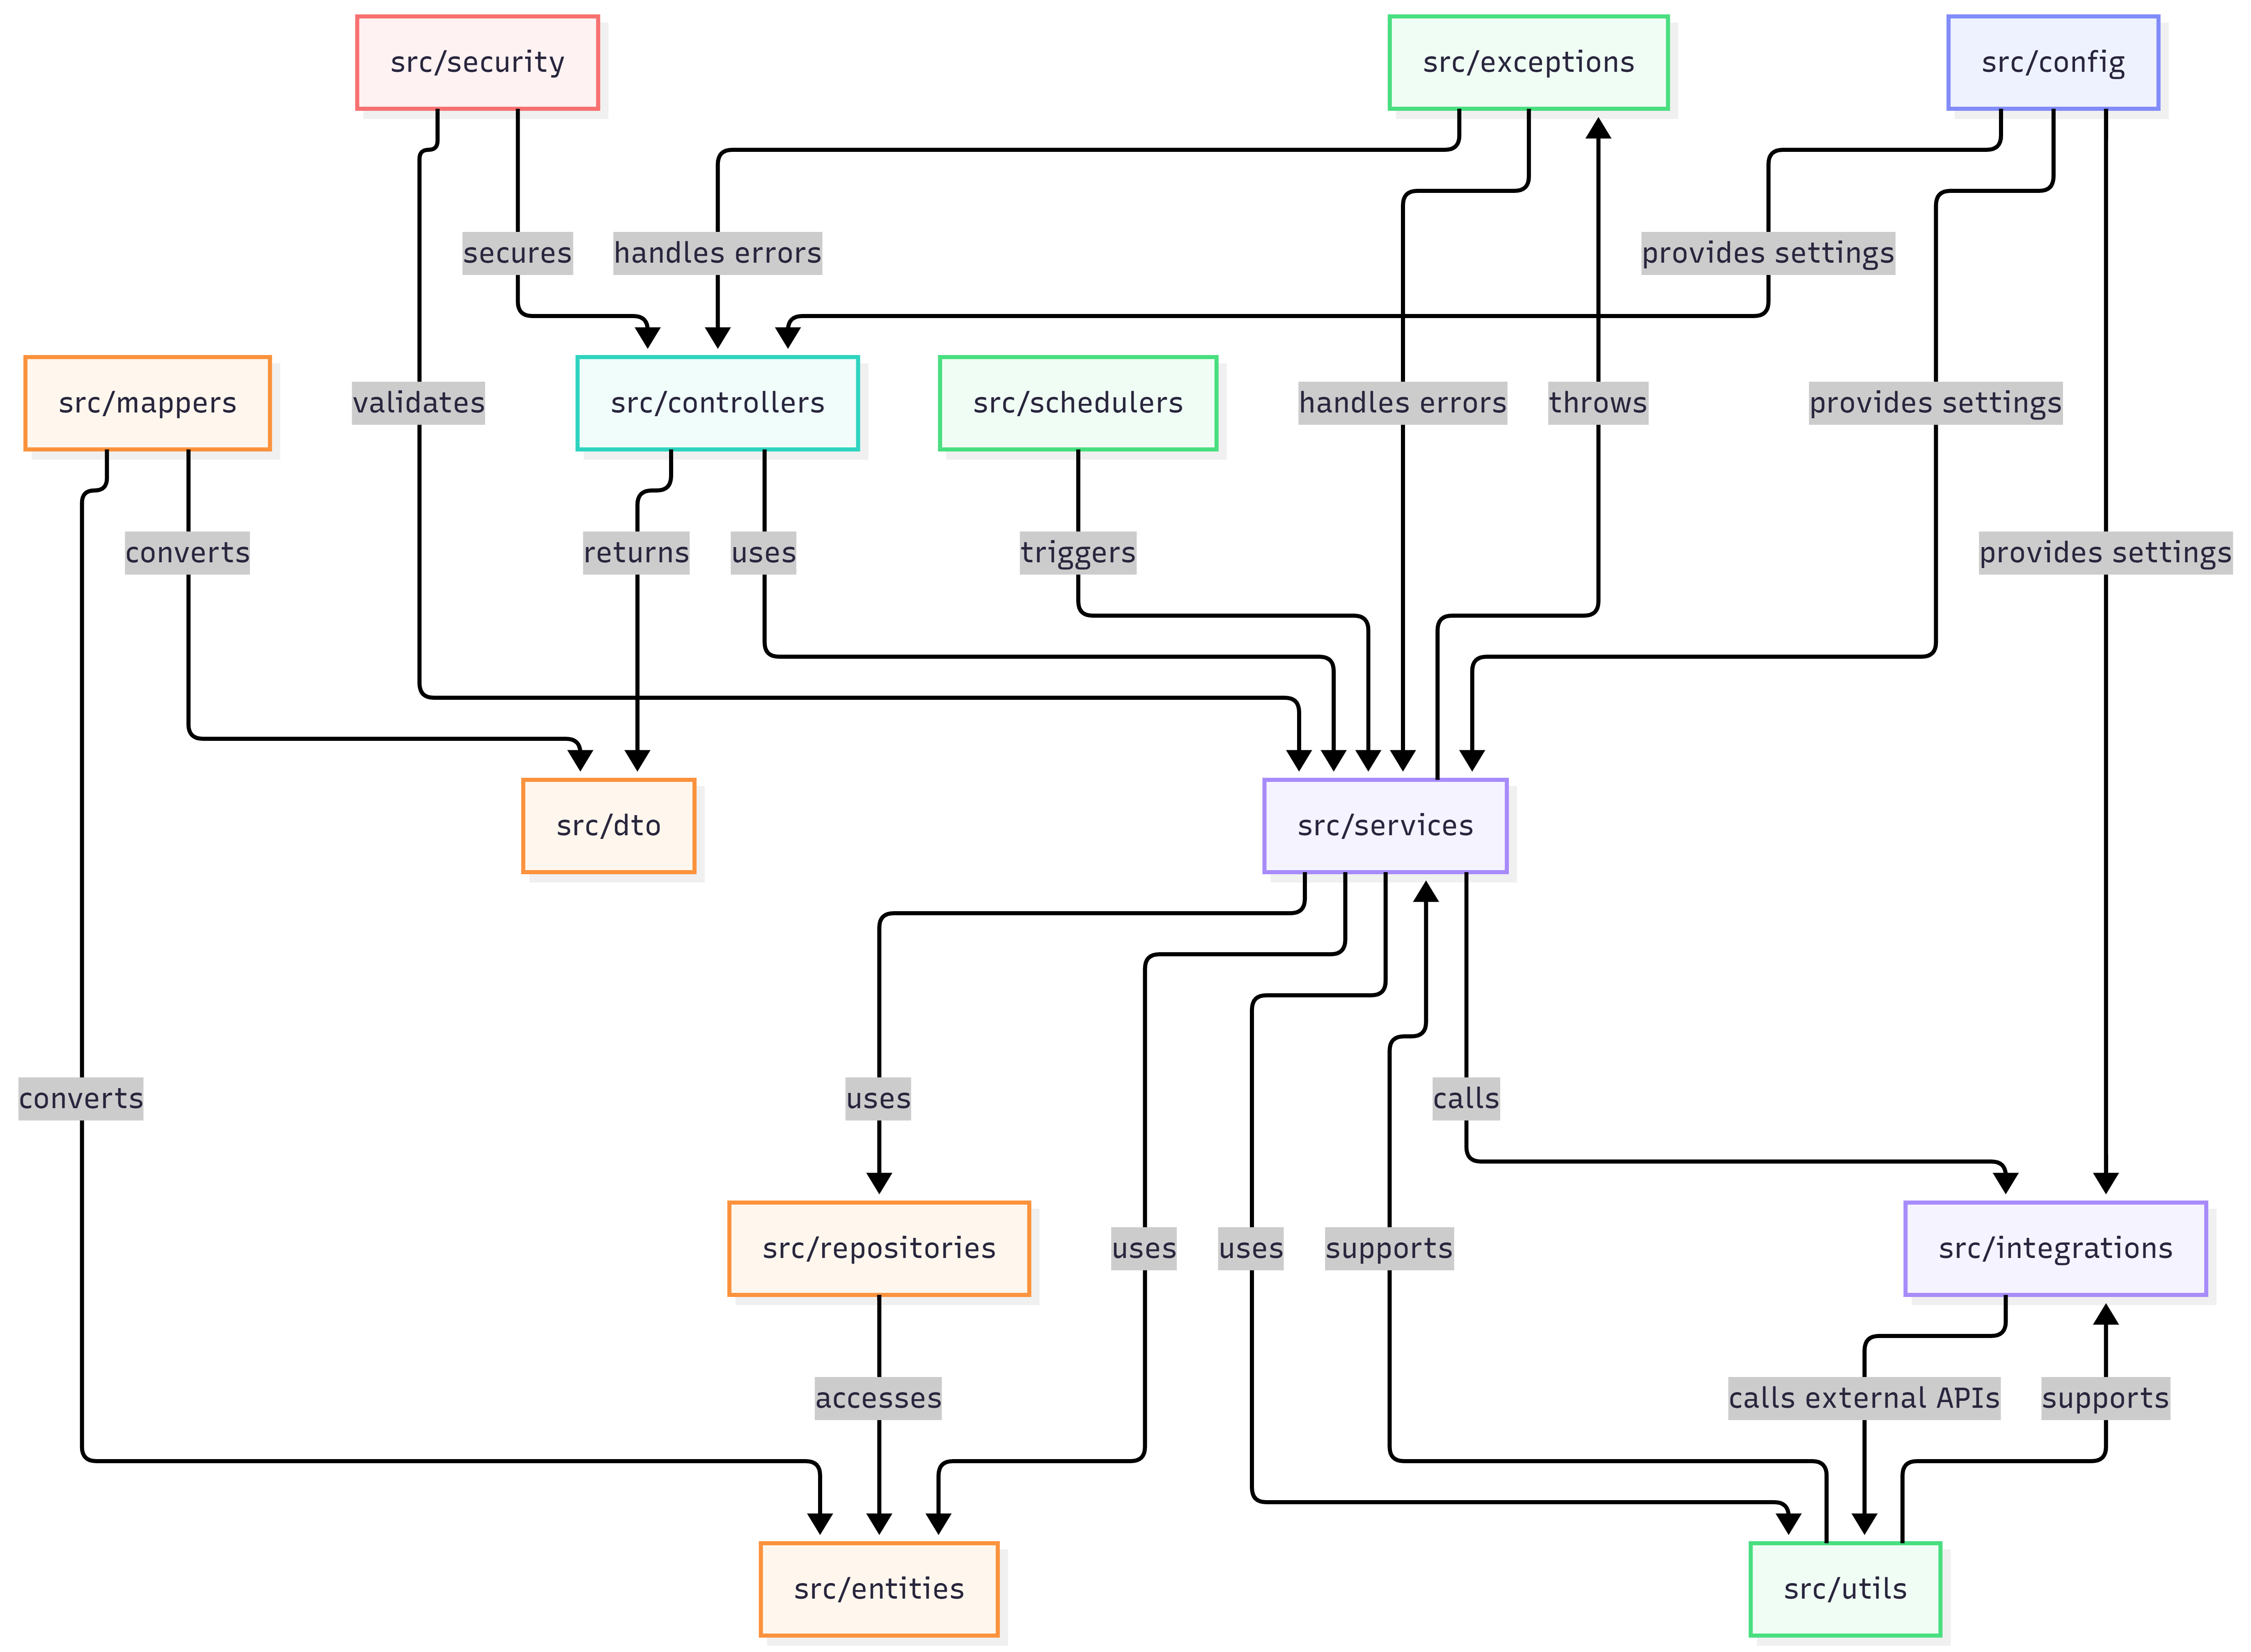
\includegraphics[width=0.95\textwidth]{images/backend.png}
    \caption{Backend Architecture Diagram}
    \label{fig:backend_architecture}
\end{figure}

\subsubsection{AI and Third-party Services}

External services are integrated to support personalization, authentication, portfolio analysis, and market data collection.

\begin{itemize}
    \item \textbf{LLM API:} Processes natural language questions and generates AI mentor responses, career advice, skill explanations, and portfolio summaries.
    \item \textbf{Google OAuth 2.0:} Allows users to authenticate with Google accounts in addition to email and password login.
    \item \textbf{GitHub API:} Retrieves public repositories, README files, programming languages, and contribution data for portfolio generation and skill analysis.
    \item \textbf{Job Portal Crawler/API:} Collects job descriptions from IT recruitment platforms to identify trending technologies and required competencies.
    \item \textbf{Cloud Deployment Platform:} Hosts frontend, backend, database, and scheduled services to ensure accessibility and scalability.
\end{itemize}

\subsection{Package Diagram}

This section describes the logical package organization of the frontend and backend applications. The structure separates responsibilities, improves maintainability, and supports future extension.

\subsubsection{Frontend Package Structure}

\renewcommand{\arraystretch}{1.3}
\setlength{\tabcolsep}{2pt}
\footnotesize
\begin{longtable}{|>{\centering\arraybackslash}p{0.65cm}|>{\raggedright\arraybackslash}p{2.8cm}|>{\raggedright\arraybackslash}p{7.6cm}|}
\caption{Frontend Package Description}
\label{tab:frontend_package_description}
\\
\hline
\textbf{No.} & \textbf{Package} & \textbf{Description} \\
\hline
\endfirsthead
\hline
\textbf{No.} & \textbf{Package} & \textbf{Description} \\
\hline
\endhead
1 & \texttt{src/app} & Contains application bootstrap files, global providers, router configuration, and application-level initialization. \\
\hline
2 & \texttt{src/pages} & Contains main screens such as dashboard, profile, roadmap, AI mentor chat, market pulse, portfolio, and administration pages. \\
\hline
3 & \texttt{src/components} & Contains reusable UI components such as buttons, forms, cards, modals, skill badges, roadmap nodes, and progress indicators. \\
\hline
4 & \texttt{src/features} & Groups feature-specific modules including authentication, career recommendation, roadmap management, skill analysis, market trends, and e-portfolio. \\
\hline
5 & \texttt{src/services} & Provides API client functions for communicating with backend endpoints and third-party integration callbacks. \\
\hline
6 & \texttt{src/hooks} & Stores custom React hooks for authentication state, form handling, roadmap progress, chat sessions, and chart data loading. \\
\hline
7 & \texttt{src/layouts} & Defines shared layouts such as student dashboard layout, administrator layout, authentication layout, and public portfolio layout. \\
\hline
8 & \texttt{src/utils} & Contains helper functions for date formatting, validation, skill score calculation, file size checking, and URL generation. \\
\hline
9 & \texttt{src/assets} & Stores static assets such as icons, images, logos, illustrations, and default avatar files. \\
\hline
10 & \texttt{src/types} & Defines TypeScript interfaces for users, roadmaps, skill nodes, job trends, chat messages, repositories, and portfolio items. \\
\hline
\end{longtable}

\subsubsection{Backend Package Structure}

\begin{longtable}{|>{\centering\arraybackslash}p{0.65cm}|>{\raggedright\arraybackslash}p{2.8cm}|>{\raggedright\arraybackslash}p{7.6cm}|}
\caption{Backend Package Description}
\label{tab:backend_package_description}
\\
\hline
\textbf{No.} & \textbf{Package} & \textbf{Description} \\
\hline
\endfirsthead
\hline
\textbf{No.} & \textbf{Package} & \textbf{Description} \\
\hline
\endhead
1 & \texttt{src/config} & Contains application configuration, environment settings, CORS configuration, scheduler configuration, and external API settings. \\
\hline
2 & \texttt{src/controllers} & Defines REST controllers that receive HTTP requests and return responses for each functional module. \\
\hline
3 & \texttt{src/security} & Handles JWT generation, token validation, password encryption, authentication filters, and role-based authorization. \\
\hline
4 & \texttt{src/services} & Contains business logic for profile management, AI mentoring, roadmap generation, skill gap analysis, market pulse, and portfolio generation. \\
\hline
5 & \texttt{src/repositories} & Provides data access interfaces for querying and updating database tables through JPA/Hibernate. \\
\hline
6 & \texttt{src/entities} & Defines domain entities such as User, StudentProfile, TechPath, SkillNode, Roadmap, JobTrend, MentorSession, and Portfolio. \\
\hline
7 & \texttt{src/dto} & Contains request and response objects used to transfer data between frontend and backend without exposing internal entities. \\
\hline
8 & \texttt{src/mappers} & Converts entities to DTOs and DTOs to entities to keep the controller, service, and persistence layers independent. \\
\hline
9 & \texttt{src/integrations} & Implements clients for LLM API, GitHub API, Google OAuth, and job portal data collection. \\
\hline
10 & \texttt{src/exceptions} & Manages custom exceptions and standardized error responses for validation, authentication, integration, and business rule errors. \\
\hline
11 & \texttt{src/utils} & Stores helper classes for file processing, text cleaning, keyword extraction, pagination, and common validation logic. \\
\hline
12 & \texttt{src/schedulers} & Contains scheduled jobs for daily job market crawling, trend analysis updates, and reminder notification generation. \\
\hline
\end{longtable}
\normalsize
\setlength{\tabcolsep}{6pt}

\section{Database Design}

The database is designed as a relational schema that maintains consistency among user accounts, student and staff profiles, career paths, skill nodes, learning resources, roadmaps, GitHub repositories, consultation sessions, AI analysis records, notifications, job trend data, and e-portfolio records. The main entities are shown in Figure~\ref{fig:erd_diagram}.

\begin{figure}[H]
    \centering
    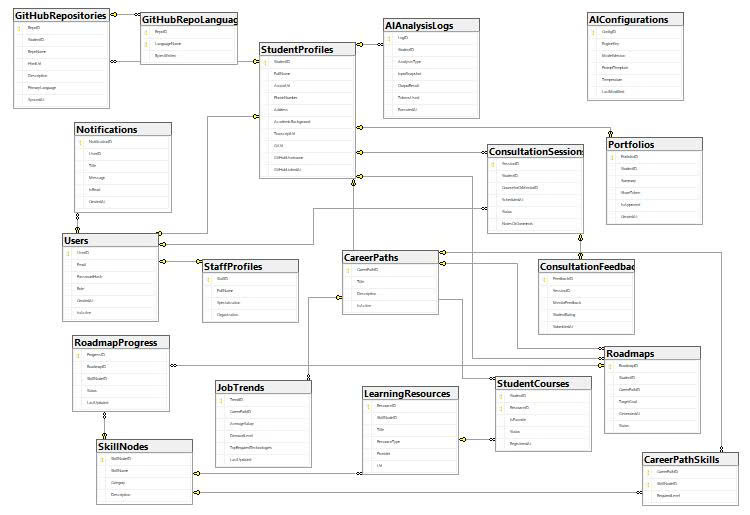
\includegraphics[width=\textwidth]{images/db design.jpg}
    \caption{Entity Relationship Diagram}
    \label{fig:erd_diagram}
\end{figure}


\subsection{Database Tables Overview}

The database contains 19 main tables. The tables cover user authentication, student and staff profiles, career paths, skill requirements, learning resources, roadmaps, portfolios, GitHub repository analysis, consultation sessions, AI configuration and analysis logs, notifications, and job market trends.

\setlength{\tabcolsep}{2pt}
\renewcommand{\arraystretch}{1.18}
\scriptsize
\subsection{Users Table}

\begin{longtable}{|>{\raggedright\arraybackslash}m{2.9cm}|>{\raggedright\arraybackslash}m{3.45cm}|>{\raggedright\arraybackslash}m{4.95cm}|}
\caption{Users Table Description}
\label{tab:users_table_description}
\\
\hline
\textbf{Field} & \textbf{Type} & \textbf{Description} \\
\hline
\endfirsthead
\hline
\textbf{Field} & \textbf{Type} & \textbf{Description} \\
\hline
\endhead
\texttt{UserID} & INT, PK, IDENTITY & Unique identifier of the user account. \\
\hline
\texttt{Email} & NVARCHAR(150), UNIQUE, NOT NULL & Email address used for login. \\
\hline
\texttt{PasswordHash} & NVARCHAR(255), NULL & Password hash; null when OAuth is used. \\
\hline
\texttt{Role} & NVARCHAR(50), NOT NULL & Role of the user in the platform. \\
\hline
\texttt{CreatedAt} & DATETIME & Account creation time. \\
\hline
\texttt{IsActive} & BIT & Account active status. \\
\hline
\end{longtable}

\subsection{CareerPaths Table}

\begin{longtable}{|>{\raggedright\arraybackslash}m{2.9cm}|>{\raggedright\arraybackslash}m{3.45cm}|>{\raggedright\arraybackslash}m{4.95cm}|}
\caption{CareerPaths Table Description}
\label{tab:career_paths_table_description}
\\
\hline
\textbf{Field} & \textbf{Type} & \textbf{Description} \\
\hline
\endfirsthead
\hline
\textbf{Field} & \textbf{Type} & \textbf{Description} \\
\hline
\endhead
\texttt{CareerPathID} & INT, PK, IDENTITY & Unique identifier of the career path. \\
\hline
\texttt{Title} & NVARCHAR(100), NOT NULL & Career path title. \\
\hline
\texttt{Description} & NVARCHAR(MAX), NULL & Detailed career path description. \\
\hline
\texttt{IsActive} & BIT & Indicates whether the career path is active. \\
\hline
\end{longtable}

\subsection{SkillNodes Table}

\begin{longtable}{|>{\raggedright\arraybackslash}m{2.9cm}|>{\raggedright\arraybackslash}m{3.45cm}|>{\raggedright\arraybackslash}m{4.95cm}|}
\caption{SkillNodes Table Description}
\label{tab:skill_nodes_table_description}
\\
\hline
\textbf{Field} & \textbf{Type} & \textbf{Description} \\
\hline
\endfirsthead
\hline
\textbf{Field} & \textbf{Type} & \textbf{Description} \\
\hline
\endhead
\texttt{SkillNodeID} & INT, PK, IDENTITY & Unique identifier of the skill node. \\
\hline
\texttt{SkillName} & NVARCHAR(100), NOT NULL & Name of the skill. \\
\hline
\texttt{Category} & NVARCHAR(100), NULL & Skill category. \\
\hline
\texttt{Description} & NVARCHAR(MAX), NULL & Detailed skill description. \\
\hline
\end{longtable}

\subsection{LearningResources Table}

\begin{longtable}{|>{\raggedright\arraybackslash}m{2.9cm}|>{\raggedright\arraybackslash}m{3.45cm}|>{\raggedright\arraybackslash}m{4.95cm}|}
\caption{LearningResources Table Description}
\label{tab:learning_resources_table_description}
\\
\hline
\textbf{Field} & \textbf{Type} & \textbf{Description} \\
\hline
\endfirsthead
\hline
\textbf{Field} & \textbf{Type} & \textbf{Description} \\
\hline
\endhead
\texttt{ResourceID} & INT, PK, IDENTITY & Unique identifier of the learning resource. \\
\hline
\texttt{SkillNodeID} & INT, FK, NOT NULL & Reference to the related skill node. \\
\hline
\texttt{Title} & NVARCHAR(255), NOT NULL & Learning resource title. \\
\hline
\texttt{ResourceType} & NVARCHAR(50), NOT NULL & Type such as Course, Book, Documentation, or Video. \\
\hline
\texttt{Provider} & NVARCHAR(100), NULL & Resource provider. \\
\hline
\texttt{Url} & NVARCHAR(500), NOT NULL & External resource URL. \\
\hline
\texttt{Description} & NVARCHAR(MAX), NULL & Additional resource description. \\
\hline
\end{longtable}

\subsection{StudentProfiles Table}

\begin{longtable}{|>{\raggedright\arraybackslash}m{2.9cm}|>{\raggedright\arraybackslash}m{3.45cm}|>{\raggedright\arraybackslash}m{4.95cm}|}
\caption{StudentProfiles Table Description}
\label{tab:student_profiles_table_description}
\\
\hline
\textbf{Field} & \textbf{Type} & \textbf{Description} \\
\hline
\endfirsthead
\hline
\textbf{Field} & \textbf{Type} & \textbf{Description} \\
\hline
\endhead
\texttt{StudentID} & INT, PK, FK & One-to-one reference to \texttt{Users(UserID)}. \\
\hline
\texttt{FullName} & NVARCHAR(100), NOT NULL & Full name of the student. \\
\hline
\texttt{AvatarUrl} & NVARCHAR(255), NULL & Student avatar image URL. \\
\hline
\texttt{PhoneNumber} & VARCHAR(20), NULL & Student phone number. \\
\hline
\texttt{Address} & NVARCHAR(255), NULL & Student address. \\
\hline
\texttt{AcademicBackground} & NVARCHAR(MAX), NULL & Academic background information. \\
\hline
\texttt{TranscriptUrl} & NVARCHAR(255), NULL & Uploaded transcript file path. \\
\hline
\texttt{CvUrl} & NVARCHAR(255), NULL & Uploaded CV file path. \\
\hline
\texttt{GitHubUsername} & NVARCHAR(100), NULL & Linked GitHub username. \\
\hline
\texttt{GitHubLinkedAt} & DATETIME, NULL & Time when GitHub was linked. \\
\hline
\end{longtable}

\subsection{StaffProfiles Table}

\begin{longtable}{|>{\raggedright\arraybackslash}m{2.9cm}|>{\raggedright\arraybackslash}m{3.45cm}|>{\raggedright\arraybackslash}m{4.95cm}|}
\caption{StaffProfiles Table Description}
\label{tab:staff_profiles_table_description}
\\
\hline
\textbf{Field} & \textbf{Type} & \textbf{Description} \\
\hline
\endfirsthead
\hline
\textbf{Field} & \textbf{Type} & \textbf{Description} \\
\hline
\endhead
\texttt{StaffID} & INT, PK, FK & One-to-one reference to \texttt{Users(UserID)}. \\
\hline
\texttt{FullName} & NVARCHAR(100), NOT NULL & Full name of the staff member. \\
\hline
\texttt{Specialization} & NVARCHAR(255), NULL & Professional specialization. \\
\hline
\texttt{Organization} & NVARCHAR(255), NULL & Organization name. \\
\hline
\texttt{Bio} & NVARCHAR(MAX), NULL & Staff biography or introduction. \\
\hline
\end{longtable}

\subsection{StudentCourses Table}

\begin{longtable}{|>{\raggedright\arraybackslash}m{2.9cm}|>{\raggedright\arraybackslash}m{3.45cm}|>{\raggedright\arraybackslash}m{4.95cm}|}
\caption{StudentCourses Table Description}
\label{tab:student_courses_table_description}
\\
\hline
\textbf{Field} & \textbf{Type} & \textbf{Description} \\
\hline
\endfirsthead
\hline
\textbf{Field} & \textbf{Type} & \textbf{Description} \\
\hline
\endhead
\texttt{StudentID} & INT, PK, FK & Reference to the student profile. \\
\hline
\texttt{ResourceID} & INT, PK, FK & Reference to the learning resource. \\
\hline
\texttt{IsFavorite} & BIT & Favorite resource flag. \\
\hline
\texttt{Status} & NVARCHAR(50) & Course status such as Enrolled or Completed. \\
\hline
\texttt{RegisteredAt} & DATETIME & Registration time. \\
\hline
\texttt{LastAccessedAt} & DATETIME, NULL & Last time the student accessed the resource. \\
\hline
\end{longtable}

\subsection{CareerPathSkills Table}

\begin{longtable}{|>{\raggedright\arraybackslash}m{2.9cm}|>{\raggedright\arraybackslash}m{3.45cm}|>{\raggedright\arraybackslash}m{4.95cm}|}
\caption{CareerPathSkills Table Description}
\label{tab:career_path_skills_table_description}
\\
\hline
\textbf{Field} & \textbf{Type} & \textbf{Description} \\
\hline
\endfirsthead
\hline
\textbf{Field} & \textbf{Type} & \textbf{Description} \\
\hline
\endhead
\texttt{CareerPathID} & INT, PK, FK & Reference to \texttt{CareerPaths(CareerPathID)}. \\
\hline
\texttt{SkillNodeID} & INT, PK, FK & Reference to \texttt{SkillNodes(SkillNodeID)}. \\
\hline
\texttt{RequiredLevel} & NVARCHAR(50) & Required level such as Basic, Intermediate, or Advanced. \\
\hline
\end{longtable}

\subsection{Roadmaps Table}

\begin{longtable}{|>{\raggedright\arraybackslash}m{2.9cm}|>{\raggedright\arraybackslash}m{3.45cm}|>{\raggedright\arraybackslash}m{4.95cm}|}
\caption{Roadmaps Table Description}
\label{tab:roadmaps_table_description}
\\
\hline
\textbf{Field} & \textbf{Type} & \textbf{Description} \\
\hline
\endfirsthead
\hline
\textbf{Field} & \textbf{Type} & \textbf{Description} \\
\hline
\endhead
\texttt{RoadmapID} & INT, PK, IDENTITY & Unique identifier of the roadmap. \\
\hline
\texttt{StudentID} & INT, FK, NOT NULL & Reference to the student profile. \\
\hline
\texttt{CareerPathID} & INT, FK, NOT NULL & Reference to the selected career path. \\
\hline
\texttt{TargetGoal} & NVARCHAR(MAX), NULL & Personal target goal. \\
\hline
\texttt{GeneratedAt} & DATETIME & Roadmap generation time. \\
\hline
\texttt{Status} & NVARCHAR(50) & Roadmap status. \\
\hline
\end{longtable}

\subsection{RoadmapProgress Table}

\begin{longtable}{|>{\raggedright\arraybackslash}m{2.9cm}|>{\raggedright\arraybackslash}m{3.45cm}|>{\raggedright\arraybackslash}m{4.95cm}|}
\caption{RoadmapProgress Table Description}
\label{tab:roadmap_progress_table_description}
\\
\hline
\textbf{Field} & \textbf{Type} & \textbf{Description} \\
\hline
\endfirsthead
\hline
\textbf{Field} & \textbf{Type} & \textbf{Description} \\
\hline
\endhead
\texttt{ProgressID} & INT, PK, IDENTITY & Unique identifier of the progress record. \\
\hline
\texttt{RoadmapID} & INT, FK, NOT NULL & Reference to the roadmap. \\
\hline
\texttt{SkillNodeID} & INT, FK, NOT NULL & Reference to the skill node. \\
\hline
\texttt{Status} & NVARCHAR(50) & Learning status. \\
\hline
\texttt{LastUpdated} & DATETIME & Last progress update time. \\
\hline
\end{longtable}

\subsection{Portfolios Table}

\begin{longtable}{|>{\raggedright\arraybackslash}m{2.9cm}|>{\raggedright\arraybackslash}m{3.45cm}|>{\raggedright\arraybackslash}m{4.95cm}|}
\caption{Portfolios Table Description}
\label{tab:portfolios_table_description}
\\
\hline
\textbf{Field} & \textbf{Type} & \textbf{Description} \\
\hline
\endfirsthead
\hline
\textbf{Field} & \textbf{Type} & \textbf{Description} \\
\hline
\endhead
\texttt{PortfolioID} & INT, PK, IDENTITY & Unique identifier of the portfolio. \\
\hline
\texttt{StudentID} & INT, UNIQUE, FK, NOT NULL & Reference to the portfolio owner. \\
\hline
\texttt{Summary} & NVARCHAR(MAX), NULL & AI-generated professional summary. \\
\hline
\texttt{ShareToken} & VARCHAR(100), UNIQUE, NULL & Token for public portfolio sharing. \\
\hline
\texttt{IsApproved} & BIT & Mentor approval status. \\
\hline
\texttt{CreatedAt} & DATETIME & Portfolio creation time. \\
\hline
\end{longtable}

\subsection{GitHubRepositories Table}

\begin{longtable}{|>{\raggedright\arraybackslash}m{2.9cm}|>{\raggedright\arraybackslash}m{3.45cm}|>{\raggedright\arraybackslash}m{4.95cm}|}
\caption{GitHubRepositories Table Description}
\label{tab:github_repositories_table_description}
\\
\hline
\textbf{Field} & \textbf{Type} & \textbf{Description} \\
\hline
\endfirsthead
\hline
\textbf{Field} & \textbf{Type} & \textbf{Description} \\
\hline
\endhead
\texttt{RepoID} & INT, PK, IDENTITY & Unique identifier of the repository record. \\
\hline
\texttt{StudentID} & INT, FK, NOT NULL & Reference to the student profile. \\
\hline
\texttt{RepoName} & NVARCHAR(150), NOT NULL & GitHub repository name. \\
\hline
\texttt{HtmlUrl} & NVARCHAR(255), NULL & Repository web URL. \\
\hline
\texttt{Description} & NVARCHAR(MAX), NULL & Repository description. \\
\hline
\texttt{PrimaryLanguage} & NVARCHAR(50), NULL & Main programming language. \\
\hline
\texttt{ReadmeContent} & NVARCHAR(MAX), NULL & README content used for portfolio analysis. \\
\hline
\texttt{SyncedAt} & DATETIME & Last synchronization time. \\
\hline
\end{longtable}

\subsection{GitHubRepoLanguages Table}

\begin{longtable}{|>{\raggedright\arraybackslash}m{2.9cm}|>{\raggedright\arraybackslash}m{3.45cm}|>{\raggedright\arraybackslash}m{4.95cm}|}
\caption{GitHubRepoLanguages Table Description}
\label{tab:github_repo_languages_table_description}
\\
\hline
\textbf{Field} & \textbf{Type} & \textbf{Description} \\
\hline
\endfirsthead
\hline
\textbf{Field} & \textbf{Type} & \textbf{Description} \\
\hline
\endhead
\texttt{RepoID} & INT, PK, FK & Reference to \texttt{GitHubRepositories(RepoID)}. \\
\hline
\texttt{LanguageName} & NVARCHAR(50), PK & Programming language name. \\
\hline
\texttt{BytesWritten} & INT, NOT NULL & Number of bytes written in the language. \\
\hline
\end{longtable}

\subsection{ConsultationSessions Table}

\begin{longtable}{|>{\raggedright\arraybackslash}m{2.9cm}|>{\raggedright\arraybackslash}m{3.45cm}|>{\raggedright\arraybackslash}m{4.95cm}|}
\caption{ConsultationSessions Table Description}
\label{tab:consultation_sessions_table_description}
\\
\hline
\textbf{Field} & \textbf{Type} & \textbf{Description} \\
\hline
\endfirsthead
\hline
\textbf{Field} & \textbf{Type} & \textbf{Description} \\
\hline
\endhead
\texttt{SessionID} & INT, PK, IDENTITY & Unique identifier of the session. \\
\hline
\texttt{StudentID} & INT, FK, NOT NULL & Reference to the student profile. \\
\hline
\texttt{CounselorOrMentorID} & INT, FK, NOT NULL & Reference to \texttt{StaffProfiles(StaffID)}. \\
\hline
\texttt{ScheduledAt} & DATETIME, NOT NULL & Scheduled consultation time. \\
\hline
\texttt{Status} & NVARCHAR(50) & Session status such as Pending, Completed, or Cancelled. \\
\hline
\texttt{MeetingLink} & NVARCHAR(255), NULL & Online meeting link. \\
\hline
\texttt{NotesOrComments} & NVARCHAR(MAX), NULL & Counselor or mentor notes and comments. \\
\hline
\end{longtable}

\subsection{ConsultationFeedbacks Table}

\begin{longtable}{|>{\raggedright\arraybackslash}m{2.9cm}|>{\raggedright\arraybackslash}m{3.45cm}|>{\raggedright\arraybackslash}m{4.95cm}|}
\caption{ConsultationFeedbacks Table Description}
\label{tab:consultation_feedbacks_table_description}
\\
\hline
\textbf{Field} & \textbf{Type} & \textbf{Description} \\
\hline
\endfirsthead
\hline
\textbf{Field} & \textbf{Type} & \textbf{Description} \\
\hline
\endhead
\texttt{FeedbackID} & INT, PK, IDENTITY & Unique identifier of the feedback record. \\
\hline
\texttt{SessionID} & INT, UNIQUE, FK, NOT NULL & Reference to the consultation session. \\
\hline
\texttt{MentorFeedback} & NVARCHAR(MAX), NULL & Feedback submitted by the mentor or counselor. \\
\hline
\texttt{StudentRating} & INT, NULL & Rating submitted by the student. \\
\hline
\texttt{SubmittedAt} & DATETIME & Feedback submission time. \\
\hline
\end{longtable}

\subsection{JobTrends Table}

\begin{longtable}{|>{\raggedright\arraybackslash}m{2.9cm}|>{\raggedright\arraybackslash}m{3.45cm}|>{\raggedright\arraybackslash}m{4.95cm}|}
\caption{JobTrends Table Description}
\label{tab:job_trends_table_description}
\\
\hline
\textbf{Field} & \textbf{Type} & \textbf{Description} \\
\hline
\endfirsthead
\hline
\textbf{Field} & \textbf{Type} & \textbf{Description} \\
\hline
\endhead
\texttt{TrendID} & INT, PK, IDENTITY & Unique identifier of the job trend record. \\
\hline
\texttt{CareerPathID} & INT, FK, NOT NULL & Reference to the career path. \\
\hline
\texttt{AverageSalary} & DECIMAL(18,2), NULL & Average salary information. \\
\hline
\texttt{DemandLevel} & NVARCHAR(50), NULL & Demand level. \\
\hline
\shortstack[l]{\texttt{TopRequired}\\\texttt{Technologies}} & NVARCHAR(MAX), NULL & Most required technologies from job market data. \\
\hline
\texttt{LastUpdated} & DATETIME & Last trend update time. \\
\hline
\end{longtable}

\subsection{AIConfigurations Table}

\begin{longtable}{|>{\raggedright\arraybackslash}m{2.9cm}|>{\raggedright\arraybackslash}m{3.45cm}|>{\raggedright\arraybackslash}m{4.95cm}|}
\caption{AIConfigurations Table Description}
\label{tab:ai_configurations_table_description}
\\
\hline
\textbf{Field} & \textbf{Type} & \textbf{Description} \\
\hline
\endfirsthead
\hline
\textbf{Field} & \textbf{Type} & \textbf{Description} \\
\hline
\endhead
\texttt{ConfigID} & INT, PK, IDENTITY & Unique identifier of the AI configuration. \\
\hline
\texttt{EngineKey} & NVARCHAR(100), UNIQUE, NOT NULL & Key used to identify the AI engine or feature. \\
\hline
\texttt{ModelVersion} & NVARCHAR(50) & Model version used by the AI feature. \\
\hline
\texttt{PromptTemplate} & NVARCHAR(MAX), NOT NULL & Prompt template for AI requests. \\
\hline
\texttt{Temperature} & FLOAT & AI generation temperature. \\
\hline
\texttt{LastModified} & DATETIME & Last configuration update time. \\
\hline
\end{longtable}

\subsection{AIAnalysisLogs Table}

\begin{longtable}{|>{\raggedright\arraybackslash}m{2.9cm}|>{\raggedright\arraybackslash}m{3.45cm}|>{\raggedright\arraybackslash}m{4.95cm}|}
\caption{AIAnalysisLogs Table Description}
\label{tab:ai_analysis_logs_table_description}
\\
\hline
\textbf{Field} & \textbf{Type} & \textbf{Description} \\
\hline
\endfirsthead
\hline
\textbf{Field} & \textbf{Type} & \textbf{Description} \\
\hline
\endhead
\texttt{LogID} & INT, PK, IDENTITY & Unique identifier of the AI analysis log. \\
\hline
\texttt{StudentID} & INT, FK, NOT NULL & Reference to the student profile. \\
\hline
\texttt{AnalysisType} & NVARCHAR(100), NOT NULL & Type of AI analysis. \\
\hline
\texttt{InputSnapshot} & NVARCHAR(MAX), NULL & Input data snapshot sent to AI. \\
\hline
\texttt{OutputResult} & NVARCHAR(MAX), NOT NULL & AI output result. \\
\hline
\texttt{TokensUsed} & INT, NULL & Number of tokens used. \\
\hline
\texttt{ExecutedAt} & DATETIME & Execution time of the AI analysis. \\
\hline
\end{longtable}

\subsection{Notifications Table}

\begin{longtable}{|>{\raggedright\arraybackslash}m{2.9cm}|>{\raggedright\arraybackslash}m{3.45cm}|>{\raggedright\arraybackslash}m{4.95cm}|}
\caption{Notifications Table Description}
\label{tab:notifications_table_description}
\\
\hline
\textbf{Field} & \textbf{Type} & \textbf{Description} \\
\hline
\endfirsthead
\hline
\textbf{Field} & \textbf{Type} & \textbf{Description} \\
\hline
\endhead
\texttt{NotificationID} & INT, PK, IDENTITY & Unique identifier of the notification. \\
\hline
\texttt{UserID} & INT, FK, NOT NULL & Reference to the receiver user. \\
\hline
\texttt{Title} & NVARCHAR(200), NOT NULL & Notification title. \\
\hline
\texttt{Message} & NVARCHAR(MAX), NOT NULL & Notification message content. \\
\hline
\texttt{IsRead} & BIT & Read status of the notification. \\
\hline
\texttt{CreatedAt} & DATETIME & Notification creation time. \\
\hline
\end{longtable}
\normalsize
\renewcommand{\arraystretch}{1.3}
\setlength{\tabcolsep}{6pt}

\setcounter{section}{2}
\setcounter{secnumdepth}{4}
\setcounter{tocdepth}{4}
\renewcommand{\theparagraph}{\thesubsubsection.\arabic{paragraph}}
\titleformat{\paragraph}[hang]
{\normalsize\bfseries}
{\theparagraph}
{0.6em}
{}
\titlespacing*{\paragraph}{0pt}{1.2ex plus .2ex}{0.8ex}

\tikzset{
    umlclass/.style={
        draw,
        rounded corners=2pt,
        fill=cyan!15,
        align=left,
        font=\scriptsize,
        text width=3.55cm,
        minimum height=2.55cm,
        inner sep=4pt
    },
    umlrelation/.style={-Latex, thick},
    participant/.style={
        draw,
        fill=cyan!20,
        align=center,
        font=\scriptsize,
        minimum width=2.35cm,
        minimum height=0.55cm
    },
    sequenceline/.style={dashed, gray!80},
    seqmessage/.style={-Latex, thick},
    seqreturn/.style={Latex-, dashed, gray!80}
}

\providecommand{\ClassDiagram}[6]{
\begin{figure}[H]
\centering
\resizebox{\textwidth}{!}{
\begin{tikzpicture}[node distance=1.0cm and 1.0cm]
    \node[umlclass] (ui) at (0,0) {
        \parbox{3.35cm}{\centering\textbf{#2}}\\
        \rule{3.35cm}{0.2pt}\\
        + displayPage()\\
        + collectInput()\\
        + showResult()
    };
    \node[umlclass] (controller) at (4.5,0) {
        \parbox{3.35cm}{\centering\textbf{#3}}\\
        \rule{3.35cm}{0.2pt}\\
        + validateRequest()\\
        + handleAction()\\
        + returnResponse()
    };
    \node[umlclass] (service) at (9.0,0) {
        \parbox{3.35cm}{\centering\textbf{#4}}\\
        \rule{3.35cm}{0.2pt}\\
        + executeUseCase()\\
        + applyRules()\\
        + buildResult()
    };
    \node[umlclass] (entity) at (0,-3.3) {
        \parbox{3.35cm}{\centering\textbf{#5}}\\
        \rule{3.35cm}{0.2pt}\\
        - id\\
        - status\\
        - createdAt
    };
    \node[umlclass] (repository) at (4.5,-3.3) {
        \parbox{3.35cm}{\centering\textbf{#6}}\\
        \rule{3.35cm}{0.2pt}\\
        + findById()\\
        + save()\\
        + update()
    };
    \node[umlclass] (gateway) at (9.0,-3.3) {
        \parbox{3.35cm}{\centering\textbf{ExternalGateway}}\\
        \rule{3.35cm}{0.2pt}\\
        + callAPI()\\
        + parseResponse()\\
        + handleFailure()
    };

    \draw[umlrelation] (ui) -- node[above,font=\scriptsize]{submit} (controller);
    \draw[umlrelation] (controller) -- node[above,font=\scriptsize]{uses} (service);
    \draw[umlrelation] (service) -- node[right,font=\scriptsize]{persists} (repository);
    \draw[umlrelation] (repository) -- node[above,font=\scriptsize]{maps} (entity);
    \draw[umlrelation] (service) -- node[right,font=\scriptsize]{integrates} (gateway);
\end{tikzpicture}
}
\caption{Class diagram for #1}
\end{figure}
}

\providecommand{\SequenceDiagram}[7]{
\begin{figure}[H]
\centering
\resizebox{\textwidth}{!}{
\begin{tikzpicture}
    \node[participant] (actor) at (0,0) {#2};
    \node[participant] (ui) at (2.8,0) {Web UI};
    \node[participant] (controller) at (5.6,0) {#4};
    \node[participant] (service) at (8.4,0) {#5};
    \node[participant] (repo) at (11.2,0) {#6};
    \node[participant] (ext) at (14.0,0) {Database/API};

    \foreach \x in {0,2.8,5.6,8.4,11.2,14.0} {
        \draw[sequenceline] (\x,-0.35) -- (\x,-7.1);
    }

    \draw[seqmessage] (0,-0.8) -- node[above,font=\scriptsize]{1. #3} (2.8,-0.8);
    \draw[seqmessage] (2.8,-1.55) -- node[above,font=\scriptsize]{2. submit request} (5.6,-1.55);
    \draw[seqmessage] (5.6,-2.3) -- node[above,font=\scriptsize]{3. validate and call service} (8.4,-2.3);
    \draw[seqmessage] (8.4,-3.05) -- node[above,font=\scriptsize]{4. load or save data} (11.2,-3.05);
    \draw[seqmessage] (11.2,-3.8) -- node[above,font=\scriptsize]{5. query/update} (14.0,-3.8);
    \draw[seqreturn] (11.2,-4.55) -- node[above,font=\scriptsize]{6. return data} (14.0,-4.55);
    \draw[seqreturn] (8.4,-5.3) -- node[above,font=\scriptsize]{7. build result} (11.2,-5.3);
    \draw[seqreturn] (5.6,-6.05) -- node[above,font=\scriptsize]{8. return response} (8.4,-6.05);
    \draw[seqreturn] (2.8,-6.8) -- node[above,font=\scriptsize]{9. #7} (5.6,-6.8);
\end{tikzpicture}
}
\caption{Sequence diagram for #1}
\end{figure}
}

\section{Detailed Design}

This section provides detailed design coverage for all 82 use cases described in Chapter~III. Each use case is traced to the related actor, database tables, controller, service, entity, repository, processing flow, exception handling, class diagram, and sequence diagram. This ensures that the detailed design is consistent with the system architecture, package design, database design, and class design presented earlier in Chapter~IV.

\subsection{Use Case to Design Coverage Summary}

\setlength{\tabcolsep}{2pt}
\scriptsize
\begin{longtable}{|>{\centering\arraybackslash}m{0.8cm}|>{\raggedright\arraybackslash}m{3.0cm}|>{\raggedright\arraybackslash}m{2.4cm}|>{\raggedright\arraybackslash}m{4.8cm}|}
\caption{Use Case to Detailed Design Coverage}
\label{tab:uc_detailed_design_coverage}
\\
\hline
\textbf{UC} & \textbf{Use Case} & \textbf{Actor} & \textbf{Design Group} \\
\hline
\endfirsthead
\hline
\textbf{UC} & \textbf{Use Case} & \textbf{Actor} & \textbf{Design Group} \\
\hline
\endhead
UC01 & Register & Student & Authentication and Account Access \\
\hline
UC02 & Login & Student & Authentication and Account Access \\
\hline
UC03 & Login with Google & Student & Authentication and Account Access \\
\hline
UC04 & Forgot Password & Student & Authentication and Account Access \\
\hline
UC05 & Logout & Student & Authentication and Account Access \\
\hline
UC06 & Manage Profile & Student & Student Profile and GitHub Integration \\
\hline
UC07 & Upload Avatar & Student & Student Profile and GitHub Integration \\
\hline
UC08 & Update Contact Information & Student & Student Profile and GitHub Integration \\
\hline
UC09 & Change Password & Student & Student Profile and GitHub Integration \\
\hline
UC10 & Upload Transcript & Student & Student Profile and GitHub Integration \\
\hline
UC11 & Upload CV & Student & Student Profile and GitHub Integration \\
\hline
UC12 & Link GitHub & Student & Student Profile and GitHub Integration \\
\hline
UC13 & Sync GitHub Repository & Student & Student Profile and GitHub Integration \\
\hline
UC14 & View GitHub Analysis & Student & Student Profile and GitHub Integration \\
\hline
UC15 & View Skill Gap Report & Student & Student Profile and GitHub Integration \\
\hline
UC16 & Select Career Role & Student & Career Path and Skill Management \\
\hline
UC17 & Update Career Goal & Student & Career Path and Skill Management \\
\hline
UC18 & View Recommended Roles & Student & Career Path and Skill Management \\
\hline
UC19 & Compare Career Paths & Student & Career Path and Skill Management \\
\hline
UC20 & View Required Skills & Student & Career Path and Skill Management \\
\hline
UC21 & Generate Learning Roadmap & Student & Learning Roadmap and Course Management \\
\hline
UC22 & View Learning Roadmap & Student & Learning Roadmap and Course Management \\
\hline
UC23 & Update Roadmap Progress & Student & Learning Roadmap and Course Management \\
\hline
UC24 & View Learning Progress & Student & Learning Roadmap and Course Management \\
\hline
UC25 & Receive Learning Reminder & Student & Learning Roadmap and Course Management \\
\hline
UC26 & Search Learning Resources & Student & Learning Roadmap and Course Management \\
\hline
UC27 & View Recommended Courses & Student & Learning Roadmap and Course Management \\
\hline
UC28 & Save Favorite Courses & Student & Learning Roadmap and Course Management \\
\hline
UC29 & Register External Course & Student & Learning Roadmap and Course Management \\
\hline
UC30 & Track Course Completion & Student & Learning Roadmap and Course Management \\
\hline
UC31 & View Market Trends & Student & Market Trend Management \\
\hline
UC32 & Search Job Opportunities & Student & Market Trend Management \\
\hline
UC33 & View Salary Information & Student & Market Trend Management \\
\hline
UC34 & View Technology Trends & Student & Market Trend Management \\
\hline
UC35 & Receive Job Recommendation & Student & Market Trend Management \\
\hline
UC36 & Chat with AI Mentor & Student & AI Mentor and Analysis Logging \\
\hline
UC37 & Ask Career Questions & Student & AI Mentor and Analysis Logging \\
\hline
UC38 & Receive AI Feedback & Student & AI Mentor and Analysis Logging \\
\hline
UC39 & Generate E-Portfolio & Student & E-Portfolio and Mentor Review \\
\hline
UC40 & Share Portfolio & Student & E-Portfolio and Mentor Review \\
\hline
UC41 & Login & Academic Counselor & Authentication and Account Access \\
\hline
UC42 & View Student Profile & Academic Counselor & Consultation and Feedback Management \\
\hline
UC43 & Review Skill Gap & Academic Counselor & Consultation and Feedback Management \\
\hline
UC44 & Recommend Career Path & Academic Counselor & Consultation and Feedback Management \\
\hline
UC45 & Recommend Courses & Academic Counselor & Consultation and Feedback Management \\
\hline
UC46 & Track Student Progress & Academic Counselor & Consultation and Feedback Management \\
\hline
UC47 & Comment Learning Plan & Academic Counselor & Consultation and Feedback Management \\
\hline
UC48 & Schedule Consultation & Academic Counselor & Consultation and Feedback Management \\
\hline
UC49 & View Consultation History & Academic Counselor & Consultation and Feedback Management \\
\hline
UC50 & Logout & Academic Counselor & Authentication and Account Access \\
\hline
UC51 & Login & Industry Mentor & Authentication and Account Access \\
\hline
UC52 & View Student Portfolio & Industry Mentor & E-Portfolio and Mentor Review \\
\hline
UC53 & Review Projects & Industry Mentor & E-Portfolio and Mentor Review \\
\hline
UC54 & Recommend Technologies & Industry Mentor & E-Portfolio and Mentor Review \\
\hline
UC55 & Give Technical Advice & Industry Mentor & E-Portfolio and Mentor Review \\
\hline
UC56 & Evaluate Progress & Industry Mentor & E-Portfolio and Mentor Review \\
\hline
UC57 & Comment Projects & Industry Mentor & E-Portfolio and Mentor Review \\
\hline
UC58 & Approve Portfolio & Industry Mentor & E-Portfolio and Mentor Review \\
\hline
UC59 & Suggest Improvements & Industry Mentor & E-Portfolio and Mentor Review \\
\hline
UC60 & Logout & Industry Mentor & Authentication and Account Access \\
\hline
UC61 & Login & Administrator & Authentication and Account Access \\
\hline
UC62 & Manage Users & Administrator & Administration and Resource Management \\
\hline
UC63 & Manage Career Roles & Administrator & Career Path and Skill Management \\
\hline
UC64 & Manage Skill Nodes & Administrator & Career Path and Skill Management \\
\hline
UC65 & Manage Courses & Administrator & Administration and Resource Management \\
\hline
UC66 & Manage Learning Resources & Administrator & Administration and Resource Management \\
\hline
UC67 & Manage Job Trend Data & Administrator & Market Trend Management \\
\hline
UC68 & Manage AI Configuration & Administrator & AI and Market Configuration \\
\hline
UC69 & Manage Reports & Administrator & Administration and Resource Management \\
\hline
UC70 & Logout & Administrator & Authentication and Account Access \\
\hline
UC71 & Analyze Transcript & AI Recommendation Engine & AI Mentor and Analysis Logging \\
\hline
UC72 & Analyze GitHub Repository & AI Recommendation Engine & AI Mentor and Analysis Logging \\
\hline
UC73 & Generate Personalized Roadmap & AI Recommendation Engine & Learning Roadmap and Course Management \\
\hline
UC74 & Analyze Skill Gap & AI Recommendation Engine & Learning Roadmap and Course Management \\
\hline
UC75 & Recommend Courses & AI Recommendation Engine & Learning Roadmap and Course Management \\
\hline
UC76 & Generate Portfolio Summary & AI Recommendation Engine & AI Mentor and Analysis Logging \\
\hline
UC77 & Authenticate User & Google OAuth & Authentication and Account Access \\
\hline
UC78 & Retrieve Repository & GitHub API & Student Profile and GitHub Integration \\
\hline
UC79 & Retrieve README & GitHub API & Student Profile and GitHub Integration \\
\hline
UC80 & Retrieve Tech Stack & GitHub API & Student Profile and GitHub Integration \\
\hline
UC81 & Retrieve Job Data & Job Portal API & Market Trend Management \\
\hline
UC82 & Analyze Market Trends & Job Portal API & Market Trend Management \\
\hline
\end{longtable}
\normalsize
\setlength{\tabcolsep}{6pt}

\subsection{Authentication and Account Access}

This group contains use cases related to authentication and account access. The design uses the layered architecture introduced in the system design: React boundary pages, Spring Boot controllers, services, repositories, database entities, and external gateways when required.

\subsubsection{UC01 Register}

\paragraph{Requirement Traceability}

\begin{itemize}
    \item \textbf{Use case ID:} UC01.
    \item \textbf{Use case name:} Register.
    \item \textbf{Actor:} Student.
    \item \textbf{Requirement description:} Create a new student account.
    \item \textbf{Related table(s):} \texttt{Users}.
\end{itemize}

\paragraph{Preconditions}

The actor has access to the corresponding interface. For protected functions, the actor must be authenticated, the account must be active, and the role stored in \texttt{Users.Role} must be allowed to perform this use case. Required master data such as career paths, skill nodes, learning resources, or staff profiles must already exist when the use case depends on them.

\paragraph{Postconditions}

The system stores the created or updated data in the related database table(s), returns a response DTO to the frontend, and records logs or notifications when the use case requires auditing, AI analysis, reminder, or integration feedback.

\paragraph{Main Processing Flow}

\begin{enumerate}
    \item The actor opens \texttt{RegisterPage} and performs the action: create a new student account..
    \item The frontend validates required fields, prepares the request DTO, and sends it to \texttt{AuthController}.
    \item \texttt{AuthController} checks authentication, authorization, request format, and path parameters.
    \item \texttt{AuthService} loads related data through \texttt{UserRepository} and applies business rules for Register.
    \item If the use case needs external data, the service calls the proper gateway such as Google OAuth, GitHub API, AI service, or job portal API.
    \item The service creates, updates, reads, or deletes records in \texttt{Users} and builds the response DTO.
    \item The frontend displays the processed result and updates the visible state for the actor.
\end{enumerate}

\paragraph{Alternative and Exception Flow}

\begin{itemize}
    \item If required input is missing or invalid, the controller returns validation errors and no database change is committed.
    \item If the actor does not have permission, the security layer returns an unauthorized or forbidden response.
    \item If a referenced record does not exist, the service returns a not-found response.
    \item If an external API fails, the service handles the failure, records the issue when applicable, and returns a retryable error message.
\end{itemize}

\paragraph{Participating Components}

\begin{itemize}
    \item \textbf{Boundary/UI -- \texttt{RegisterPage}:} collects input and displays the final result for Register.
    \item \textbf{Controller -- \texttt{AuthController}:} receives REST requests and validates request DTOs.
    \item \textbf{Service -- \texttt{AuthService}:} coordinates business logic, integration calls, and transaction boundaries.
    \item \textbf{Entity -- \texttt{User}:} represents the main persisted domain object.
    \item \textbf{Repository -- \texttt{UserRepository}:} provides data access operations for the related table(s).
\end{itemize}

\paragraph{Class Diagram}

\ClassDiagram
{UC01 Register}
{RegisterPage}
{AuthController}
{AuthService}
{User}
{UserRepository}

\paragraph{Sequence Diagram}

\SequenceDiagram
{UC01 Register}
{Student}
{create a new student account.}
{AuthController}
{AuthService}
{UserRepository}
{display processed result}

\subsubsection{UC02 Login}

\paragraph{Requirement Traceability}

\begin{itemize}
    \item \textbf{Use case ID:} UC02.
    \item \textbf{Use case name:} Login.
    \item \textbf{Actor:} Student.
    \item \textbf{Requirement description:} Login using email and password.
    \item \textbf{Related table(s):} \texttt{Users}.
\end{itemize}

\paragraph{Preconditions}

The actor has access to the corresponding interface. For protected functions, the actor must be authenticated, the account must be active, and the role stored in \texttt{Users.Role} must be allowed to perform this use case. Required master data such as career paths, skill nodes, learning resources, or staff profiles must already exist when the use case depends on them.

\paragraph{Postconditions}

The system stores the created or updated data in the related database table(s), returns a response DTO to the frontend, and records logs or notifications when the use case requires auditing, AI analysis, reminder, or integration feedback.

\paragraph{Main Processing Flow}

\begin{enumerate}
    \item The actor opens \texttt{LoginPage} and performs the action: login using email and password..
    \item The frontend validates required fields, prepares the request DTO, and sends it to \texttt{AuthController}.
    \item \texttt{AuthController} checks authentication, authorization, request format, and path parameters.
    \item \texttt{AuthService} loads related data through \texttt{UserRepository} and applies business rules for Login.
    \item If the use case needs external data, the service calls the proper gateway such as Google OAuth, GitHub API, AI service, or job portal API.
    \item The service creates, updates, reads, or deletes records in \texttt{Users} and builds the response DTO.
    \item The frontend displays the processed result and updates the visible state for the actor.
\end{enumerate}

\paragraph{Alternative and Exception Flow}

\begin{itemize}
    \item If required input is missing or invalid, the controller returns validation errors and no database change is committed.
    \item If the actor does not have permission, the security layer returns an unauthorized or forbidden response.
    \item If a referenced record does not exist, the service returns a not-found response.
    \item If an external API fails, the service handles the failure, records the issue when applicable, and returns a retryable error message.
\end{itemize}

\paragraph{Participating Components}

\begin{itemize}
    \item \textbf{Boundary/UI -- \texttt{LoginPage}:} collects input and displays the final result for Login.
    \item \textbf{Controller -- \texttt{AuthController}:} receives REST requests and validates request DTOs.
    \item \textbf{Service -- \texttt{AuthService}:} coordinates business logic, integration calls, and transaction boundaries.
    \item \textbf{Entity -- \texttt{User}:} represents the main persisted domain object.
    \item \textbf{Repository -- \texttt{UserRepository}:} provides data access operations for the related table(s).
\end{itemize}

\paragraph{Class Diagram}

\ClassDiagram
{UC02 Login}
{LoginPage}
{AuthController}
{AuthService}
{User}
{UserRepository}

\paragraph{Sequence Diagram}

\SequenceDiagram
{UC02 Login}
{Student}
{login using email and password.}
{AuthController}
{AuthService}
{UserRepository}
{display processed result}

\subsubsection{UC03 Login with Google}

\paragraph{Requirement Traceability}

\begin{itemize}
    \item \textbf{Use case ID:} UC03.
    \item \textbf{Use case name:} Login with Google.
    \item \textbf{Actor:} Student.
    \item \textbf{Requirement description:} Authenticate via Google OAuth.
    \item \textbf{Related table(s):} \texttt{Users}.
\end{itemize}

\paragraph{Preconditions}

The actor has access to the corresponding interface. For protected functions, the actor must be authenticated, the account must be active, and the role stored in \texttt{Users.Role} must be allowed to perform this use case. Required master data such as career paths, skill nodes, learning resources, or staff profiles must already exist when the use case depends on them.

\paragraph{Postconditions}

The system stores the created or updated data in the related database table(s), returns a response DTO to the frontend, and records logs or notifications when the use case requires auditing, AI analysis, reminder, or integration feedback.

\paragraph{Main Processing Flow}

\begin{enumerate}
    \item The actor opens \texttt{LoginwithGooglePage} and performs the action: authenticate via Google OAuth..
    \item The frontend validates required fields, prepares the request DTO, and sends it to \texttt{AuthController}.
    \item \texttt{AuthController} checks authentication, authorization, request format, and path parameters.
    \item \texttt{AuthService} loads related data through \texttt{UserRepository} and applies business rules for Login with Google.
    \item If the use case needs external data, the service calls the proper gateway such as Google OAuth, GitHub API, AI service, or job portal API.
    \item The service creates, updates, reads, or deletes records in \texttt{Users} and builds the response DTO.
    \item The frontend displays the processed result and updates the visible state for the actor.
\end{enumerate}

\paragraph{Alternative and Exception Flow}

\begin{itemize}
    \item If required input is missing or invalid, the controller returns validation errors and no database change is committed.
    \item If the actor does not have permission, the security layer returns an unauthorized or forbidden response.
    \item If a referenced record does not exist, the service returns a not-found response.
    \item If an external API fails, the service handles the failure, records the issue when applicable, and returns a retryable error message.
\end{itemize}

\paragraph{Participating Components}

\begin{itemize}
    \item \textbf{Boundary/UI -- \texttt{LoginwithGooglePage}:} collects input and displays the final result for Login with Google.
    \item \textbf{Controller -- \texttt{AuthController}:} receives REST requests and validates request DTOs.
    \item \textbf{Service -- \texttt{AuthService}:} coordinates business logic, integration calls, and transaction boundaries.
    \item \textbf{Entity -- \texttt{User}:} represents the main persisted domain object.
    \item \textbf{Repository -- \texttt{UserRepository}:} provides data access operations for the related table(s).
\end{itemize}

\paragraph{Class Diagram}

\ClassDiagram
{UC03 Login with Google}
{LoginwithGooglePage}
{AuthController}
{AuthService}
{User}
{UserRepository}

\paragraph{Sequence Diagram}

\SequenceDiagram
{UC03 Login with Google}
{Student}
{authenticate via Google OAuth.}
{AuthController}
{AuthService}
{UserRepository}
{display processed result}

\subsubsection{UC04 Forgot Password}

\paragraph{Requirement Traceability}

\begin{itemize}
    \item \textbf{Use case ID:} UC04.
    \item \textbf{Use case name:} Forgot Password.
    \item \textbf{Actor:} Student.
    \item \textbf{Requirement description:} Recover forgotten password.
    \item \textbf{Related table(s):} \texttt{Users}.
\end{itemize}

\paragraph{Preconditions}

The actor has access to the corresponding interface. For protected functions, the actor must be authenticated, the account must be active, and the role stored in \texttt{Users.Role} must be allowed to perform this use case. Required master data such as career paths, skill nodes, learning resources, or staff profiles must already exist when the use case depends on them.

\paragraph{Postconditions}

The system stores the created or updated data in the related database table(s), returns a response DTO to the frontend, and records logs or notifications when the use case requires auditing, AI analysis, reminder, or integration feedback.

\paragraph{Main Processing Flow}

\begin{enumerate}
    \item The actor opens \texttt{ForgotPasswordPage} and performs the action: recover forgotten password..
    \item The frontend validates required fields, prepares the request DTO, and sends it to \texttt{AuthController}.
    \item \texttt{AuthController} checks authentication, authorization, request format, and path parameters.
    \item \texttt{AuthService} loads related data through \texttt{UserRepository} and applies business rules for Forgot Password.
    \item If the use case needs external data, the service calls the proper gateway such as Google OAuth, GitHub API, AI service, or job portal API.
    \item The service creates, updates, reads, or deletes records in \texttt{Users} and builds the response DTO.
    \item The frontend displays the processed result and updates the visible state for the actor.
\end{enumerate}

\paragraph{Alternative and Exception Flow}

\begin{itemize}
    \item If required input is missing or invalid, the controller returns validation errors and no database change is committed.
    \item If the actor does not have permission, the security layer returns an unauthorized or forbidden response.
    \item If a referenced record does not exist, the service returns a not-found response.
    \item If an external API fails, the service handles the failure, records the issue when applicable, and returns a retryable error message.
\end{itemize}

\paragraph{Participating Components}

\begin{itemize}
    \item \textbf{Boundary/UI -- \texttt{ForgotPasswordPage}:} collects input and displays the final result for Forgot Password.
    \item \textbf{Controller -- \texttt{AuthController}:} receives REST requests and validates request DTOs.
    \item \textbf{Service -- \texttt{AuthService}:} coordinates business logic, integration calls, and transaction boundaries.
    \item \textbf{Entity -- \texttt{User}:} represents the main persisted domain object.
    \item \textbf{Repository -- \texttt{UserRepository}:} provides data access operations for the related table(s).
\end{itemize}

\paragraph{Class Diagram}

\ClassDiagram
{UC04 Forgot Password}
{ForgotPasswordPage}
{AuthController}
{AuthService}
{User}
{UserRepository}

\paragraph{Sequence Diagram}

\SequenceDiagram
{UC04 Forgot Password}
{Student}
{recover forgotten password.}
{AuthController}
{AuthService}
{UserRepository}
{display processed result}

\subsubsection{UC05 Logout}

\paragraph{Requirement Traceability}

\begin{itemize}
    \item \textbf{Use case ID:} UC05.
    \item \textbf{Use case name:} Logout.
    \item \textbf{Actor:} Student.
    \item \textbf{Requirement description:} Logout from the system.
    \item \textbf{Related table(s):} \texttt{Users}.
\end{itemize}

\paragraph{Preconditions}

The actor has access to the corresponding interface. For protected functions, the actor must be authenticated, the account must be active, and the role stored in \texttt{Users.Role} must be allowed to perform this use case. Required master data such as career paths, skill nodes, learning resources, or staff profiles must already exist when the use case depends on them.

\paragraph{Postconditions}

The system stores the created or updated data in the related database table(s), returns a response DTO to the frontend, and records logs or notifications when the use case requires auditing, AI analysis, reminder, or integration feedback.

\paragraph{Main Processing Flow}

\begin{enumerate}
    \item The actor opens \texttt{LogoutPage} and performs the action: logout from the system..
    \item The frontend validates required fields, prepares the request DTO, and sends it to \texttt{AuthController}.
    \item \texttt{AuthController} checks authentication, authorization, request format, and path parameters.
    \item \texttt{AuthService} loads related data through \texttt{UserRepository} and applies business rules for Logout.
    \item If the use case needs external data, the service calls the proper gateway such as Google OAuth, GitHub API, AI service, or job portal API.
    \item The service creates, updates, reads, or deletes records in \texttt{Users} and builds the response DTO.
    \item The frontend displays the processed result and updates the visible state for the actor.
\end{enumerate}

\paragraph{Alternative and Exception Flow}

\begin{itemize}
    \item If required input is missing or invalid, the controller returns validation errors and no database change is committed.
    \item If the actor does not have permission, the security layer returns an unauthorized or forbidden response.
    \item If a referenced record does not exist, the service returns a not-found response.
    \item If an external API fails, the service handles the failure, records the issue when applicable, and returns a retryable error message.
\end{itemize}

\paragraph{Participating Components}

\begin{itemize}
    \item \textbf{Boundary/UI -- \texttt{LogoutPage}:} collects input and displays the final result for Logout.
    \item \textbf{Controller -- \texttt{AuthController}:} receives REST requests and validates request DTOs.
    \item \textbf{Service -- \texttt{AuthService}:} coordinates business logic, integration calls, and transaction boundaries.
    \item \textbf{Entity -- \texttt{User}:} represents the main persisted domain object.
    \item \textbf{Repository -- \texttt{UserRepository}:} provides data access operations for the related table(s).
\end{itemize}

\paragraph{Class Diagram}

\ClassDiagram
{UC05 Logout}
{LogoutPage}
{AuthController}
{AuthService}
{User}
{UserRepository}

\paragraph{Sequence Diagram}

\SequenceDiagram
{UC05 Logout}
{Student}
{logout from the system.}
{AuthController}
{AuthService}
{UserRepository}
{display processed result}

\subsection{Student Profile and GitHub Integration}

This group contains use cases related to student profile and github integration. The design uses the layered architecture introduced in the system design: React boundary pages, Spring Boot controllers, services, repositories, database entities, and external gateways when required.

\subsubsection{UC06 Manage Profile}

\paragraph{Requirement Traceability}

\begin{itemize}
    \item \textbf{Use case ID:} UC06.
    \item \textbf{Use case name:} Manage Profile.
    \item \textbf{Actor:} Student.
    \item \textbf{Requirement description:} Update personal information.
    \item \textbf{Related table(s):} \texttt{StudentProfiles}.
\end{itemize}

\paragraph{Preconditions}

The actor has access to the corresponding interface. For protected functions, the actor must be authenticated, the account must be active, and the role stored in \texttt{Users.Role} must be allowed to perform this use case. Required master data such as career paths, skill nodes, learning resources, or staff profiles must already exist when the use case depends on them.

\paragraph{Postconditions}

The system stores the created or updated data in the related database table(s), returns a response DTO to the frontend, and records logs or notifications when the use case requires auditing, AI analysis, reminder, or integration feedback.

\paragraph{Main Processing Flow}

\begin{enumerate}
    \item The actor opens \texttt{ManageProfilePage} and performs the action: update personal information..
    \item The frontend validates required fields, prepares the request DTO, and sends it to \texttt{ProfileController}.
    \item \texttt{ProfileController} checks authentication, authorization, request format, and path parameters.
    \item \texttt{ProfileService} loads related data through \texttt{StudentProfileRepo} and applies business rules for Manage Profile.
    \item If the use case needs external data, the service calls the proper gateway such as Google OAuth, GitHub API, AI service, or job portal API.
    \item The service creates, updates, reads, or deletes records in \texttt{StudentProfiles} and builds the response DTO.
    \item The frontend displays the processed result and updates the visible state for the actor.
\end{enumerate}

\paragraph{Alternative and Exception Flow}

\begin{itemize}
    \item If required input is missing or invalid, the controller returns validation errors and no database change is committed.
    \item If the actor does not have permission, the security layer returns an unauthorized or forbidden response.
    \item If a referenced record does not exist, the service returns a not-found response.
    \item If an external API fails, the service handles the failure, records the issue when applicable, and returns a retryable error message.
\end{itemize}

\paragraph{Participating Components}

\begin{itemize}
    \item \textbf{Boundary/UI -- \texttt{ManageProfilePage}:} collects input and displays the final result for Manage Profile.
    \item \textbf{Controller -- \texttt{ProfileController}:} receives REST requests and validates request DTOs.
    \item \textbf{Service -- \texttt{ProfileService}:} coordinates business logic, integration calls, and transaction boundaries.
    \item \textbf{Entity -- \texttt{StudentProfile}:} represents the main persisted domain object.
    \item \textbf{Repository -- \texttt{StudentProfileRepo}:} provides data access operations for the related table(s).
\end{itemize}

\paragraph{Class Diagram}

\ClassDiagram
{UC06 Manage Profile}
{ManageProfilePage}
{ProfileController}
{ProfileService}
{StudentProfile}
{StudentProfileRepo}

\paragraph{Sequence Diagram}

\SequenceDiagram
{UC06 Manage Profile}
{Student}
{update personal information.}
{ProfileController}
{ProfileService}
{StudentProfileRepo}
{display processed result}

\subsubsection{UC07 Upload Avatar}

\paragraph{Requirement Traceability}

\begin{itemize}
    \item \textbf{Use case ID:} UC07.
    \item \textbf{Use case name:} Upload Avatar.
    \item \textbf{Actor:} Student.
    \item \textbf{Requirement description:} Upload profile image.
    \item \textbf{Related table(s):} \texttt{StudentProfiles}.
\end{itemize}

\paragraph{Preconditions}

The actor has access to the corresponding interface. For protected functions, the actor must be authenticated, the account must be active, and the role stored in \texttt{Users.Role} must be allowed to perform this use case. Required master data such as career paths, skill nodes, learning resources, or staff profiles must already exist when the use case depends on them.

\paragraph{Postconditions}

The system stores the created or updated data in the related database table(s), returns a response DTO to the frontend, and records logs or notifications when the use case requires auditing, AI analysis, reminder, or integration feedback.

\paragraph{Main Processing Flow}

\begin{enumerate}
    \item The actor opens \texttt{UploadAvatarPage} and performs the action: upload profile image..
    \item The frontend validates required fields, prepares the request DTO, and sends it to \texttt{ProfileController}.
    \item \texttt{ProfileController} checks authentication, authorization, request format, and path parameters.
    \item \texttt{ProfileService} loads related data through \texttt{StudentProfileRepo} and applies business rules for Upload Avatar.
    \item If the use case needs external data, the service calls the proper gateway such as Google OAuth, GitHub API, AI service, or job portal API.
    \item The service creates, updates, reads, or deletes records in \texttt{StudentProfiles} and builds the response DTO.
    \item The frontend displays the processed result and updates the visible state for the actor.
\end{enumerate}

\paragraph{Alternative and Exception Flow}

\begin{itemize}
    \item If required input is missing or invalid, the controller returns validation errors and no database change is committed.
    \item If the actor does not have permission, the security layer returns an unauthorized or forbidden response.
    \item If a referenced record does not exist, the service returns a not-found response.
    \item If an external API fails, the service handles the failure, records the issue when applicable, and returns a retryable error message.
\end{itemize}

\paragraph{Participating Components}

\begin{itemize}
    \item \textbf{Boundary/UI -- \texttt{UploadAvatarPage}:} collects input and displays the final result for Upload Avatar.
    \item \textbf{Controller -- \texttt{ProfileController}:} receives REST requests and validates request DTOs.
    \item \textbf{Service -- \texttt{ProfileService}:} coordinates business logic, integration calls, and transaction boundaries.
    \item \textbf{Entity -- \texttt{StudentProfile}:} represents the main persisted domain object.
    \item \textbf{Repository -- \texttt{StudentProfileRepo}:} provides data access operations for the related table(s).
\end{itemize}

\paragraph{Class Diagram}

\ClassDiagram
{UC07 Upload Avatar}
{UploadAvatarPage}
{ProfileController}
{ProfileService}
{StudentProfile}
{StudentProfileRepo}

\paragraph{Sequence Diagram}

\SequenceDiagram
{UC07 Upload Avatar}
{Student}
{upload profile image.}
{ProfileController}
{ProfileService}
{StudentProfileRepo}
{display processed result}

\subsubsection{UC08 Update Contact Information}

\paragraph{Requirement Traceability}

\begin{itemize}
    \item \textbf{Use case ID:} UC08.
    \item \textbf{Use case name:} Update Contact Information.
    \item \textbf{Actor:} Student.
    \item \textbf{Requirement description:} Edit phone number and address.
    \item \textbf{Related table(s):} \texttt{StudentProfiles}.
\end{itemize}

\paragraph{Preconditions}

The actor has access to the corresponding interface. For protected functions, the actor must be authenticated, the account must be active, and the role stored in \texttt{Users.Role} must be allowed to perform this use case. Required master data such as career paths, skill nodes, learning resources, or staff profiles must already exist when the use case depends on them.

\paragraph{Postconditions}

The system stores the created or updated data in the related database table(s), returns a response DTO to the frontend, and records logs or notifications when the use case requires auditing, AI analysis, reminder, or integration feedback.

\paragraph{Main Processing Flow}

\begin{enumerate}
    \item The actor opens \texttt{UpdateContactInforPage} and performs the action: edit phone number and address..
    \item The frontend validates required fields, prepares the request DTO, and sends it to \texttt{ProfileController}.
    \item \texttt{ProfileController} checks authentication, authorization, request format, and path parameters.
    \item \texttt{ProfileService} loads related data through \texttt{StudentProfileRepo} and applies business rules for Update Contact Information.
    \item If the use case needs external data, the service calls the proper gateway such as Google OAuth, GitHub API, AI service, or job portal API.
    \item The service creates, updates, reads, or deletes records in \texttt{StudentProfiles} and builds the response DTO.
    \item The frontend displays the processed result and updates the visible state for the actor.
\end{enumerate}

\paragraph{Alternative and Exception Flow}

\begin{itemize}
    \item If required input is missing or invalid, the controller returns validation errors and no database change is committed.
    \item If the actor does not have permission, the security layer returns an unauthorized or forbidden response.
    \item If a referenced record does not exist, the service returns a not-found response.
    \item If an external API fails, the service handles the failure, records the issue when applicable, and returns a retryable error message.
\end{itemize}

\paragraph{Participating Components}

\begin{itemize}
    \item \textbf{Boundary/UI -- \texttt{UpdateContactInforPage}:} collects input and displays the final result for Update Contact Information.
    \item \textbf{Controller -- \texttt{ProfileController}:} receives REST requests and validates request DTOs.
    \item \textbf{Service -- \texttt{ProfileService}:} coordinates business logic, integration calls, and transaction boundaries.
    \item \textbf{Entity -- \texttt{StudentProfile}:} represents the main persisted domain object.
    \item \textbf{Repository -- \texttt{StudentProfileRepo}:} provides data access operations for the related table(s).
\end{itemize}

\paragraph{Class Diagram}

\ClassDiagram
{UC08 Update Contact Information}
{UpdateContactInforPage}
{ProfileController}
{ProfileService}
{StudentProfile}
{StudentProfileRepo}

\paragraph{Sequence Diagram}

\SequenceDiagram
{UC08 Update Contact Information}
{Student}
{edit phone number and address.}
{ProfileController}
{ProfileService}
{StudentProfileRepo}
{display processed result}

\subsubsection{UC09 Change Password}

\paragraph{Requirement Traceability}

\begin{itemize}
    \item \textbf{Use case ID:} UC09.
    \item \textbf{Use case name:} Change Password.
    \item \textbf{Actor:} Student.
    \item \textbf{Requirement description:} Update account password.
    \item \textbf{Related table(s):} \texttt{StudentProfiles}.
\end{itemize}

\paragraph{Preconditions}

The actor has access to the corresponding interface. For protected functions, the actor must be authenticated, the account must be active, and the role stored in \texttt{Users.Role} must be allowed to perform this use case. Required master data such as career paths, skill nodes, learning resources, or staff profiles must already exist when the use case depends on them.

\paragraph{Postconditions}

The system stores the created or updated data in the related database table(s), returns a response DTO to the frontend, and records logs or notifications when the use case requires auditing, AI analysis, reminder, or integration feedback.

\paragraph{Main Processing Flow}

\begin{enumerate}
    \item The actor opens \texttt{ChangePasswordPage} and performs the action: update account password..
    \item The frontend validates required fields, prepares the request DTO, and sends it to \texttt{ProfileController}.
    \item \texttt{ProfileController} checks authentication, authorization, request format, and path parameters.
    \item \texttt{ProfileService} loads related data through \texttt{StudentProfileRepo} and applies business rules for Change Password.
    \item If the use case needs external data, the service calls the proper gateway such as Google OAuth, GitHub API, AI service, or job portal API.
    \item The service creates, updates, reads, or deletes records in \texttt{StudentProfiles} and builds the response DTO.
    \item The frontend displays the processed result and updates the visible state for the actor.
\end{enumerate}

\paragraph{Alternative and Exception Flow}

\begin{itemize}
    \item If required input is missing or invalid, the controller returns validation errors and no database change is committed.
    \item If the actor does not have permission, the security layer returns an unauthorized or forbidden response.
    \item If a referenced record does not exist, the service returns a not-found response.
    \item If an external API fails, the service handles the failure, records the issue when applicable, and returns a retryable error message.
\end{itemize}

\paragraph{Participating Components}

\begin{itemize}
    \item \textbf{Boundary/UI -- \texttt{ChangePasswordPage}:} collects input and displays the final result for Change Password.
    \item \textbf{Controller -- \texttt{ProfileController}:} receives REST requests and validates request DTOs.
    \item \textbf{Service -- \texttt{ProfileService}:} coordinates business logic, integration calls, and transaction boundaries.
    \item \textbf{Entity -- \texttt{StudentProfile}:} represents the main persisted domain object.
    \item \textbf{Repository -- \texttt{StudentProfileRepo}:} provides data access operations for the related table(s).
\end{itemize}

\paragraph{Class Diagram}

\ClassDiagram
{UC09 Change Password}
{ChangePasswordPage}
{ProfileController}
{ProfileService}
{StudentProfile}
{StudentProfileRepo}

\paragraph{Sequence Diagram}

\SequenceDiagram
{UC09 Change Password}
{Student}
{update account password.}
{ProfileController}
{ProfileService}
{StudentProfileRepo}
{display processed result}

\subsubsection{UC10 Upload Transcript}

\paragraph{Requirement Traceability}

\begin{itemize}
    \item \textbf{Use case ID:} UC10.
    \item \textbf{Use case name:} Upload Transcript.
    \item \textbf{Actor:} Student.
    \item \textbf{Requirement description:} Upload academic transcript.
    \item \textbf{Related table(s):} \texttt{StudentProfiles}.
\end{itemize}

\paragraph{Preconditions}

The actor has access to the corresponding interface. For protected functions, the actor must be authenticated, the account must be active, and the role stored in \texttt{Users.Role} must be allowed to perform this use case. Required master data such as career paths, skill nodes, learning resources, or staff profiles must already exist when the use case depends on them.

\paragraph{Postconditions}

The system stores the created or updated data in the related database table(s), returns a response DTO to the frontend, and records logs or notifications when the use case requires auditing, AI analysis, reminder, or integration feedback.

\paragraph{Main Processing Flow}

\begin{enumerate}
    \item The actor opens \texttt{UploadTranscriptPage} and performs the action: upload academic transcript..
    \item The frontend validates required fields, prepares the request DTO, and sends it to \texttt{ProfileController}.
    \item \texttt{ProfileController} checks authentication, authorization, request format, and path parameters.
    \item \texttt{ProfileService} loads related data through \texttt{StudentProfileRepo} and applies business rules for Upload Transcript.
    \item If the use case needs external data, the service calls the proper gateway such as Google OAuth, GitHub API, AI service, or job portal API.
    \item The service creates, updates, reads, or deletes records in \texttt{StudentProfiles} and builds the response DTO.
    \item The frontend displays the processed result and updates the visible state for the actor.
\end{enumerate}

\paragraph{Alternative and Exception Flow}

\begin{itemize}
    \item If required input is missing or invalid, the controller returns validation errors and no database change is committed.
    \item If the actor does not have permission, the security layer returns an unauthorized or forbidden response.
    \item If a referenced record does not exist, the service returns a not-found response.
    \item If an external API fails, the service handles the failure, records the issue when applicable, and returns a retryable error message.
\end{itemize}

\paragraph{Participating Components}

\begin{itemize}
    \item \textbf{Boundary/UI -- \texttt{UploadTranscriptPage}:} collects input and displays the final result for Upload Transcript.
    \item \textbf{Controller -- \texttt{ProfileController}:} receives REST requests and validates request DTOs.
    \item \textbf{Service -- \texttt{ProfileService}:} coordinates business logic, integration calls, and transaction boundaries.
    \item \textbf{Entity -- \texttt{StudentProfile}:} represents the main persisted domain object.
    \item \textbf{Repository -- \texttt{StudentProfileRepo}:} provides data access operations for the related table(s).
\end{itemize}

\paragraph{Class Diagram}

\ClassDiagram
{UC10 Upload Transcript}
{UploadTranscriptPage}
{ProfileController}
{ProfileService}
{StudentProfile}
{StudentProfileRepo}

\paragraph{Sequence Diagram}

\SequenceDiagram
{UC10 Upload Transcript}
{Student}
{upload academic transcript.}
{ProfileController}
{ProfileService}
{StudentProfileRepo}
{display processed result}

\subsubsection{UC11 Upload CV}

\paragraph{Requirement Traceability}

\begin{itemize}
    \item \textbf{Use case ID:} UC11.
    \item \textbf{Use case name:} Upload CV.
    \item \textbf{Actor:} Student.
    \item \textbf{Requirement description:} Upload curriculum vitae.
    \item \textbf{Related table(s):} \texttt{StudentProfiles}.
\end{itemize}

\paragraph{Preconditions}

The actor has access to the corresponding interface. For protected functions, the actor must be authenticated, the account must be active, and the role stored in \texttt{Users.Role} must be allowed to perform this use case. Required master data such as career paths, skill nodes, learning resources, or staff profiles must already exist when the use case depends on them.

\paragraph{Postconditions}

The system stores the created or updated data in the related database table(s), returns a response DTO to the frontend, and records logs or notifications when the use case requires auditing, AI analysis, reminder, or integration feedback.

\paragraph{Main Processing Flow}

\begin{enumerate}
    \item The actor opens \texttt{UploadCVPage} and performs the action: upload curriculum vitae..
    \item The frontend validates required fields, prepares the request DTO, and sends it to \texttt{ProfileController}.
    \item \texttt{ProfileController} checks authentication, authorization, request format, and path parameters.
    \item \texttt{ProfileService} loads related data through \texttt{StudentProfileRepo} and applies business rules for Upload CV.
    \item If the use case needs external data, the service calls the proper gateway such as Google OAuth, GitHub API, AI service, or job portal API.
    \item The service creates, updates, reads, or deletes records in \texttt{StudentProfiles} and builds the response DTO.
    \item The frontend displays the processed result and updates the visible state for the actor.
\end{enumerate}

\paragraph{Alternative and Exception Flow}

\begin{itemize}
    \item If required input is missing or invalid, the controller returns validation errors and no database change is committed.
    \item If the actor does not have permission, the security layer returns an unauthorized or forbidden response.
    \item If a referenced record does not exist, the service returns a not-found response.
    \item If an external API fails, the service handles the failure, records the issue when applicable, and returns a retryable error message.
\end{itemize}

\paragraph{Participating Components}

\begin{itemize}
    \item \textbf{Boundary/UI -- \texttt{UploadCVPage}:} collects input and displays the final result for Upload CV.
    \item \textbf{Controller -- \texttt{ProfileController}:} receives REST requests and validates request DTOs.
    \item \textbf{Service -- \texttt{ProfileService}:} coordinates business logic, integration calls, and transaction boundaries.
    \item \textbf{Entity -- \texttt{StudentProfile}:} represents the main persisted domain object.
    \item \textbf{Repository -- \texttt{StudentProfileRepo}:} provides data access operations for the related table(s).
\end{itemize}

\paragraph{Class Diagram}

\ClassDiagram
{UC11 Upload CV}
{UploadCVPage}
{ProfileController}
{ProfileService}
{StudentProfile}
{StudentProfileRepo}

\paragraph{Sequence Diagram}

\SequenceDiagram
{UC11 Upload CV}
{Student}
{upload curriculum vitae.}
{ProfileController}
{ProfileService}
{StudentProfileRepo}
{display processed result}

\subsubsection{UC12 Link GitHub}

\paragraph{Requirement Traceability}

\begin{itemize}
    \item \textbf{Use case ID:} UC12.
    \item \textbf{Use case name:} Link GitHub.
    \item \textbf{Actor:} Student.
    \item \textbf{Requirement description:} Connect GitHub account.
    \item \textbf{Related table(s):} \texttt{StudentProfiles, GitHubRepositories, GitHubRepoLanguages}.
\end{itemize}

\paragraph{Preconditions}

The actor has access to the corresponding interface. For protected functions, the actor must be authenticated, the account must be active, and the role stored in \texttt{Users.Role} must be allowed to perform this use case. Required master data such as career paths, skill nodes, learning resources, or staff profiles must already exist when the use case depends on them.

\paragraph{Postconditions}

The system stores the created or updated data in the related database table(s), returns a response DTO to the frontend, and records logs or notifications when the use case requires auditing, AI analysis, reminder, or integration feedback.

\paragraph{Main Processing Flow}

\begin{enumerate}
    \item The actor opens \texttt{LinkGitHubPage} and performs the action: connect GitHub account..
    \item The frontend validates required fields, prepares the request DTO, and sends it to \texttt{GitHubController}.
    \item \texttt{GitHubController} checks authentication, authorization, request format, and path parameters.
    \item \texttt{GitHubSyncService} loads related data through \texttt{GitHubRepositoryRepo} and applies business rules for Link GitHub.
    \item If the use case needs external data, the service calls the proper gateway such as Google OAuth, GitHub API, AI service, or job portal API.
    \item The service creates, updates, reads, or deletes records in \texttt{StudentProfiles, GitHubRepositories, GitHubRepoLanguages} and builds the response DTO.
    \item The frontend displays the processed result and updates the visible state for the actor.
\end{enumerate}

\paragraph{Alternative and Exception Flow}

\begin{itemize}
    \item If required input is missing or invalid, the controller returns validation errors and no database change is committed.
    \item If the actor does not have permission, the security layer returns an unauthorized or forbidden response.
    \item If a referenced record does not exist, the service returns a not-found response.
    \item If an external API fails, the service handles the failure, records the issue when applicable, and returns a retryable error message.
\end{itemize}

\paragraph{Participating Components}

\begin{itemize}
    \item \textbf{Boundary/UI -- \texttt{LinkGitHubPage}:} collects input and displays the final result for Link GitHub.
    \item \textbf{Controller -- \texttt{GitHubController}:} receives REST requests and validates request DTOs.
    \item \textbf{Service -- \texttt{GitHubSyncService}:} coordinates business logic, integration calls, and transaction boundaries.
    \item \textbf{Entity -- \texttt{GitHubRepository}:} represents the main persisted domain object.
    \item \textbf{Repository -- \texttt{GitHubRepositoryRepo}:} provides data access operations for the related table(s).
\end{itemize}

\paragraph{Class Diagram}

\ClassDiagram
{UC12 Link GitHub}
{LinkGitHubPage}
{GitHubController}
{GitHubSyncService}
{GitHubRepository}
{GitHubRepositoryRepo}

\paragraph{Sequence Diagram}

\SequenceDiagram
{UC12 Link GitHub}
{Student}
{connect GitHub account.}
{GitHubController}
{GitHubSyncService}
{GitHubRepositoryRepo}
{display processed result}

\subsubsection{UC13 Sync GitHub Repository}

\paragraph{Requirement Traceability}

\begin{itemize}
    \item \textbf{Use case ID:} UC13.
    \item \textbf{Use case name:} Sync GitHub Repository.
    \item \textbf{Actor:} Student.
    \item \textbf{Requirement description:} Synchronize repository information.
    \item \textbf{Related table(s):} \texttt{StudentProfiles, GitHubRepositories, GitHubRepoLanguages}.
\end{itemize}

\paragraph{Preconditions}

The actor has access to the corresponding interface. For protected functions, the actor must be authenticated, the account must be active, and the role stored in \texttt{Users.Role} must be allowed to perform this use case. Required master data such as career paths, skill nodes, learning resources, or staff profiles must already exist when the use case depends on them.

\paragraph{Postconditions}

The system stores the created or updated data in the related database table(s), returns a response DTO to the frontend, and records logs or notifications when the use case requires auditing, AI analysis, reminder, or integration feedback.

\paragraph{Main Processing Flow}

\begin{enumerate}
    \item The actor opens \texttt{SyncGitHubRepositoPage} and performs the action: synchronize repository information..
    \item The frontend validates required fields, prepares the request DTO, and sends it to \texttt{GitHubController}.
    \item \texttt{GitHubController} checks authentication, authorization, request format, and path parameters.
    \item \texttt{GitHubSyncService} loads related data through \texttt{GitHubRepositoryRepo} and applies business rules for Sync GitHub Repository.
    \item If the use case needs external data, the service calls the proper gateway such as Google OAuth, GitHub API, AI service, or job portal API.
    \item The service creates, updates, reads, or deletes records in \texttt{StudentProfiles, GitHubRepositories, GitHubRepoLanguages} and builds the response DTO.
    \item The frontend displays the processed result and updates the visible state for the actor.
\end{enumerate}

\paragraph{Alternative and Exception Flow}

\begin{itemize}
    \item If required input is missing or invalid, the controller returns validation errors and no database change is committed.
    \item If the actor does not have permission, the security layer returns an unauthorized or forbidden response.
    \item If a referenced record does not exist, the service returns a not-found response.
    \item If an external API fails, the service handles the failure, records the issue when applicable, and returns a retryable error message.
\end{itemize}

\paragraph{Participating Components}

\begin{itemize}
    \item \textbf{Boundary/UI -- \texttt{SyncGitHubRepositoPage}:} collects input and displays the final result for Sync GitHub Repository.
    \item \textbf{Controller -- \texttt{GitHubController}:} receives REST requests and validates request DTOs.
    \item \textbf{Service -- \texttt{GitHubSyncService}:} coordinates business logic, integration calls, and transaction boundaries.
    \item \textbf{Entity -- \texttt{GitHubRepository}:} represents the main persisted domain object.
    \item \textbf{Repository -- \texttt{GitHubRepositoryRepo}:} provides data access operations for the related table(s).
\end{itemize}

\paragraph{Class Diagram}

\ClassDiagram
{UC13 Sync GitHub Repository}
{SyncGitHubRepositoPage}
{GitHubController}
{GitHubSyncService}
{GitHubRepository}
{GitHubRepositoryRepo}

\paragraph{Sequence Diagram}

\SequenceDiagram
{UC13 Sync GitHub Repository}
{Student}
{synchronize repository information.}
{GitHubController}
{GitHubSyncService}
{GitHubRepositoryRepo}
{display processed result}

\subsubsection{UC14 View GitHub Analysis}

\paragraph{Requirement Traceability}

\begin{itemize}
    \item \textbf{Use case ID:} UC14.
    \item \textbf{Use case name:} View GitHub Analysis.
    \item \textbf{Actor:} Student.
    \item \textbf{Requirement description:} View programming skill analysis.
    \item \textbf{Related table(s):} \texttt{StudentProfiles, GitHubRepositories, GitHubRepoLanguages}.
\end{itemize}

\paragraph{Preconditions}

The actor has access to the corresponding interface. For protected functions, the actor must be authenticated, the account must be active, and the role stored in \texttt{Users.Role} must be allowed to perform this use case. Required master data such as career paths, skill nodes, learning resources, or staff profiles must already exist when the use case depends on them.

\paragraph{Postconditions}

The system stores the created or updated data in the related database table(s), returns a response DTO to the frontend, and records logs or notifications when the use case requires auditing, AI analysis, reminder, or integration feedback.

\paragraph{Main Processing Flow}

\begin{enumerate}
    \item The actor opens \texttt{ViewGitHubAnalysisPage} and performs the action: view programming skill analysis..
    \item The frontend validates required fields, prepares the request DTO, and sends it to \texttt{GitHubController}.
    \item \texttt{GitHubController} checks authentication, authorization, request format, and path parameters.
    \item \texttt{GitHubSyncService} loads related data through \texttt{GitHubRepositoryRepo} and applies business rules for View GitHub Analysis.
    \item If the use case needs external data, the service calls the proper gateway such as Google OAuth, GitHub API, AI service, or job portal API.
    \item The service creates, updates, reads, or deletes records in \texttt{StudentProfiles, GitHubRepositories, GitHubRepoLanguages} and builds the response DTO.
    \item The frontend displays the processed result and updates the visible state for the actor.
\end{enumerate}

\paragraph{Alternative and Exception Flow}

\begin{itemize}
    \item If required input is missing or invalid, the controller returns validation errors and no database change is committed.
    \item If the actor does not have permission, the security layer returns an unauthorized or forbidden response.
    \item If a referenced record does not exist, the service returns a not-found response.
    \item If an external API fails, the service handles the failure, records the issue when applicable, and returns a retryable error message.
\end{itemize}

\paragraph{Participating Components}

\begin{itemize}
    \item \textbf{Boundary/UI -- \texttt{ViewGitHubAnalysisPage}:} collects input and displays the final result for View GitHub Analysis.
    \item \textbf{Controller -- \texttt{GitHubController}:} receives REST requests and validates request DTOs.
    \item \textbf{Service -- \texttt{GitHubSyncService}:} coordinates business logic, integration calls, and transaction boundaries.
    \item \textbf{Entity -- \texttt{GitHubRepository}:} represents the main persisted domain object.
    \item \textbf{Repository -- \texttt{GitHubRepositoryRepo}:} provides data access operations for the related table(s).
\end{itemize}

\paragraph{Class Diagram}

\ClassDiagram
{UC14 View GitHub Analysis}
{ViewGitHubAnalysisPage}
{GitHubController}
{GitHubSyncService}
{GitHubRepository}
{GitHubRepositoryRepo}

\paragraph{Sequence Diagram}

\SequenceDiagram
{UC14 View GitHub Analysis}
{Student}
{view programming skill analysis.}
{GitHubController}
{GitHubSyncService}
{GitHubRepositoryRepo}
{display processed result}

\subsubsection{UC15 View Skill Gap Report}

\paragraph{Requirement Traceability}

\begin{itemize}
    \item \textbf{Use case ID:} UC15.
    \item \textbf{Use case name:} View Skill Gap Report.
    \item \textbf{Actor:} Student.
    \item \textbf{Requirement description:} View missing skills analysis.
    \item \textbf{Related table(s):} \texttt{StudentProfiles}.
\end{itemize}

\paragraph{Preconditions}

The actor has access to the corresponding interface. For protected functions, the actor must be authenticated, the account must be active, and the role stored in \texttt{Users.Role} must be allowed to perform this use case. Required master data such as career paths, skill nodes, learning resources, or staff profiles must already exist when the use case depends on them.

\paragraph{Postconditions}

The system stores the created or updated data in the related database table(s), returns a response DTO to the frontend, and records logs or notifications when the use case requires auditing, AI analysis, reminder, or integration feedback.

\paragraph{Main Processing Flow}

\begin{enumerate}
    \item The actor opens \texttt{ViewSkillGapReportPage} and performs the action: view missing skills analysis..
    \item The frontend validates required fields, prepares the request DTO, and sends it to \texttt{ProfileController}.
    \item \texttt{ProfileController} checks authentication, authorization, request format, and path parameters.
    \item \texttt{ProfileService} loads related data through \texttt{StudentProfileRepo} and applies business rules for View Skill Gap Report.
    \item If the use case needs external data, the service calls the proper gateway such as Google OAuth, GitHub API, AI service, or job portal API.
    \item The service creates, updates, reads, or deletes records in \texttt{StudentProfiles} and builds the response DTO.
    \item The frontend displays the processed result and updates the visible state for the actor.
\end{enumerate}

\paragraph{Alternative and Exception Flow}

\begin{itemize}
    \item If required input is missing or invalid, the controller returns validation errors and no database change is committed.
    \item If the actor does not have permission, the security layer returns an unauthorized or forbidden response.
    \item If a referenced record does not exist, the service returns a not-found response.
    \item If an external API fails, the service handles the failure, records the issue when applicable, and returns a retryable error message.
\end{itemize}

\paragraph{Participating Components}

\begin{itemize}
    \item \textbf{Boundary/UI -- \texttt{ViewSkillGapReportPage}:} collects input and displays the final result for View Skill Gap Report.
    \item \textbf{Controller -- \texttt{ProfileController}:} receives REST requests and validates request DTOs.
    \item \textbf{Service -- \texttt{ProfileService}:} coordinates business logic, integration calls, and transaction boundaries.
    \item \textbf{Entity -- \texttt{StudentProfile}:} represents the main persisted domain object.
    \item \textbf{Repository -- \texttt{StudentProfileRepo}:} provides data access operations for the related table(s).
\end{itemize}

\paragraph{Class Diagram}

\ClassDiagram
{UC15 View Skill Gap Report}
{ViewSkillGapReportPage}
{ProfileController}
{ProfileService}
{StudentProfile}
{StudentProfileRepo}

\paragraph{Sequence Diagram}

\SequenceDiagram
{UC15 View Skill Gap Report}
{Student}
{view missing skills analysis.}
{ProfileController}
{ProfileService}
{StudentProfileRepo}
{display processed result}

\subsection{Career Path and Skill Management}

This group contains use cases related to career path and skill management. The design uses the layered architecture introduced in the system design: React boundary pages, Spring Boot controllers, services, repositories, database entities, and external gateways when required.

\subsubsection{UC16 Select Career Role}

\paragraph{Requirement Traceability}

\begin{itemize}
    \item \textbf{Use case ID:} UC16.
    \item \textbf{Use case name:} Select Career Role.
    \item \textbf{Actor:} Student.
    \item \textbf{Requirement description:} Select desired career path.
    \item \textbf{Related table(s):} \texttt{CareerPaths, SkillNodes, CareerPathSkills}.
\end{itemize}

\paragraph{Preconditions}

The actor has access to the corresponding interface. For protected functions, the actor must be authenticated, the account must be active, and the role stored in \texttt{Users.Role} must be allowed to perform this use case. Required master data such as career paths, skill nodes, learning resources, or staff profiles must already exist when the use case depends on them.

\paragraph{Postconditions}

The system stores the created or updated data in the related database table(s), returns a response DTO to the frontend, and records logs or notifications when the use case requires auditing, AI analysis, reminder, or integration feedback.

\paragraph{Main Processing Flow}

\begin{enumerate}
    \item The actor opens \texttt{SelectCareerRolePage} and performs the action: select desired career path..
    \item The frontend validates required fields, prepares the request DTO, and sends it to \texttt{CareerPathController}.
    \item \texttt{CareerPathController} checks authentication, authorization, request format, and path parameters.
    \item \texttt{CareerPathService} loads related data through \texttt{CareerPathRepository} and applies business rules for Select Career Role.
    \item If the use case needs external data, the service calls the proper gateway such as Google OAuth, GitHub API, AI service, or job portal API.
    \item The service creates, updates, reads, or deletes records in \texttt{CareerPaths, SkillNodes, CareerPathSkills} and builds the response DTO.
    \item The frontend displays the processed result and updates the visible state for the actor.
\end{enumerate}

\paragraph{Alternative and Exception Flow}

\begin{itemize}
    \item If required input is missing or invalid, the controller returns validation errors and no database change is committed.
    \item If the actor does not have permission, the security layer returns an unauthorized or forbidden response.
    \item If a referenced record does not exist, the service returns a not-found response.
    \item If an external API fails, the service handles the failure, records the issue when applicable, and returns a retryable error message.
\end{itemize}

\paragraph{Participating Components}

\begin{itemize}
    \item \textbf{Boundary/UI -- \texttt{SelectCareerRolePage}:} collects input and displays the final result for Select Career Role.
    \item \textbf{Controller -- \texttt{CareerPathController}:} receives REST requests and validates request DTOs.
    \item \textbf{Service -- \texttt{CareerPathService}:} coordinates business logic, integration calls, and transaction boundaries.
    \item \textbf{Entity -- \texttt{CareerPath}:} represents the main persisted domain object.
    \item \textbf{Repository -- \texttt{CareerPathRepository}:} provides data access operations for the related table(s).
\end{itemize}

\paragraph{Class Diagram}

\ClassDiagram
{UC16 Select Career Role}
{SelectCareerRolePage}
{CareerPathController}
{CareerPathService}
{CareerPath}
{CareerPathRepository}

\paragraph{Sequence Diagram}

\SequenceDiagram
{UC16 Select Career Role}
{Student}
{select desired career path.}
{CareerPathController}
{CareerPathService}
{CareerPathRepository}
{display processed result}

\subsubsection{UC17 Update Career Goal}

\paragraph{Requirement Traceability}

\begin{itemize}
    \item \textbf{Use case ID:} UC17.
    \item \textbf{Use case name:} Update Career Goal.
    \item \textbf{Actor:} Student.
    \item \textbf{Requirement description:} Modify career objective.
    \item \textbf{Related table(s):} \texttt{CareerPaths, SkillNodes, CareerPathSkills}.
\end{itemize}

\paragraph{Preconditions}

The actor has access to the corresponding interface. For protected functions, the actor must be authenticated, the account must be active, and the role stored in \texttt{Users.Role} must be allowed to perform this use case. Required master data such as career paths, skill nodes, learning resources, or staff profiles must already exist when the use case depends on them.

\paragraph{Postconditions}

The system stores the created or updated data in the related database table(s), returns a response DTO to the frontend, and records logs or notifications when the use case requires auditing, AI analysis, reminder, or integration feedback.

\paragraph{Main Processing Flow}

\begin{enumerate}
    \item The actor opens \texttt{UpdateCareerGoalPage} and performs the action: modify career objective..
    \item The frontend validates required fields, prepares the request DTO, and sends it to \texttt{CareerPathController}.
    \item \texttt{CareerPathController} checks authentication, authorization, request format, and path parameters.
    \item \texttt{CareerPathService} loads related data through \texttt{CareerPathRepository} and applies business rules for Update Career Goal.
    \item If the use case needs external data, the service calls the proper gateway such as Google OAuth, GitHub API, AI service, or job portal API.
    \item The service creates, updates, reads, or deletes records in \texttt{CareerPaths, SkillNodes, CareerPathSkills} and builds the response DTO.
    \item The frontend displays the processed result and updates the visible state for the actor.
\end{enumerate}

\paragraph{Alternative and Exception Flow}

\begin{itemize}
    \item If required input is missing or invalid, the controller returns validation errors and no database change is committed.
    \item If the actor does not have permission, the security layer returns an unauthorized or forbidden response.
    \item If a referenced record does not exist, the service returns a not-found response.
    \item If an external API fails, the service handles the failure, records the issue when applicable, and returns a retryable error message.
\end{itemize}

\paragraph{Participating Components}

\begin{itemize}
    \item \textbf{Boundary/UI -- \texttt{UpdateCareerGoalPage}:} collects input and displays the final result for Update Career Goal.
    \item \textbf{Controller -- \texttt{CareerPathController}:} receives REST requests and validates request DTOs.
    \item \textbf{Service -- \texttt{CareerPathService}:} coordinates business logic, integration calls, and transaction boundaries.
    \item \textbf{Entity -- \texttt{CareerPath}:} represents the main persisted domain object.
    \item \textbf{Repository -- \texttt{CareerPathRepository}:} provides data access operations for the related table(s).
\end{itemize}

\paragraph{Class Diagram}

\ClassDiagram
{UC17 Update Career Goal}
{UpdateCareerGoalPage}
{CareerPathController}
{CareerPathService}
{CareerPath}
{CareerPathRepository}

\paragraph{Sequence Diagram}

\SequenceDiagram
{UC17 Update Career Goal}
{Student}
{modify career objective.}
{CareerPathController}
{CareerPathService}
{CareerPathRepository}
{display processed result}

\subsubsection{UC18 View Recommended Roles}

\paragraph{Requirement Traceability}

\begin{itemize}
    \item \textbf{Use case ID:} UC18.
    \item \textbf{Use case name:} View Recommended Roles.
    \item \textbf{Actor:} Student.
    \item \textbf{Requirement description:} View suggested careers.
    \item \textbf{Related table(s):} \texttt{CareerPaths, SkillNodes, CareerPathSkills}.
\end{itemize}

\paragraph{Preconditions}

The actor has access to the corresponding interface. For protected functions, the actor must be authenticated, the account must be active, and the role stored in \texttt{Users.Role} must be allowed to perform this use case. Required master data such as career paths, skill nodes, learning resources, or staff profiles must already exist when the use case depends on them.

\paragraph{Postconditions}

The system stores the created or updated data in the related database table(s), returns a response DTO to the frontend, and records logs or notifications when the use case requires auditing, AI analysis, reminder, or integration feedback.

\paragraph{Main Processing Flow}

\begin{enumerate}
    \item The actor opens \texttt{ViewRecommendedRolPage} and performs the action: view suggested careers..
    \item The frontend validates required fields, prepares the request DTO, and sends it to \texttt{CareerPathController}.
    \item \texttt{CareerPathController} checks authentication, authorization, request format, and path parameters.
    \item \texttt{CareerPathService} loads related data through \texttt{CareerPathRepository} and applies business rules for View Recommended Roles.
    \item If the use case needs external data, the service calls the proper gateway such as Google OAuth, GitHub API, AI service, or job portal API.
    \item The service creates, updates, reads, or deletes records in \texttt{CareerPaths, SkillNodes, CareerPathSkills} and builds the response DTO.
    \item The frontend displays the processed result and updates the visible state for the actor.
\end{enumerate}

\paragraph{Alternative and Exception Flow}

\begin{itemize}
    \item If required input is missing or invalid, the controller returns validation errors and no database change is committed.
    \item If the actor does not have permission, the security layer returns an unauthorized or forbidden response.
    \item If a referenced record does not exist, the service returns a not-found response.
    \item If an external API fails, the service handles the failure, records the issue when applicable, and returns a retryable error message.
\end{itemize}

\paragraph{Participating Components}

\begin{itemize}
    \item \textbf{Boundary/UI -- \texttt{ViewRecommendedRolPage}:} collects input and displays the final result for View Recommended Roles.
    \item \textbf{Controller -- \texttt{CareerPathController}:} receives REST requests and validates request DTOs.
    \item \textbf{Service -- \texttt{CareerPathService}:} coordinates business logic, integration calls, and transaction boundaries.
    \item \textbf{Entity -- \texttt{CareerPath}:} represents the main persisted domain object.
    \item \textbf{Repository -- \texttt{CareerPathRepository}:} provides data access operations for the related table(s).
\end{itemize}

\paragraph{Class Diagram}

\ClassDiagram
{UC18 View Recommended Roles}
{ViewRecommendedRolPage}
{CareerPathController}
{CareerPathService}
{CareerPath}
{CareerPathRepository}

\paragraph{Sequence Diagram}

\SequenceDiagram
{UC18 View Recommended Roles}
{Student}
{view suggested careers.}
{CareerPathController}
{CareerPathService}
{CareerPathRepository}
{display processed result}

\subsubsection{UC19 Compare Career Paths}

\paragraph{Requirement Traceability}

\begin{itemize}
    \item \textbf{Use case ID:} UC19.
    \item \textbf{Use case name:} Compare Career Paths.
    \item \textbf{Actor:} Student.
    \item \textbf{Requirement description:} Compare different career options.
    \item \textbf{Related table(s):} \texttt{CareerPaths, SkillNodes, CareerPathSkills}.
\end{itemize}

\paragraph{Preconditions}

The actor has access to the corresponding interface. For protected functions, the actor must be authenticated, the account must be active, and the role stored in \texttt{Users.Role} must be allowed to perform this use case. Required master data such as career paths, skill nodes, learning resources, or staff profiles must already exist when the use case depends on them.

\paragraph{Postconditions}

The system stores the created or updated data in the related database table(s), returns a response DTO to the frontend, and records logs or notifications when the use case requires auditing, AI analysis, reminder, or integration feedback.

\paragraph{Main Processing Flow}

\begin{enumerate}
    \item The actor opens \texttt{CompareCareerPathsPage} and performs the action: compare different career options..
    \item The frontend validates required fields, prepares the request DTO, and sends it to \texttt{CareerPathController}.
    \item \texttt{CareerPathController} checks authentication, authorization, request format, and path parameters.
    \item \texttt{CareerPathService} loads related data through \texttt{CareerPathRepository} and applies business rules for Compare Career Paths.
    \item If the use case needs external data, the service calls the proper gateway such as Google OAuth, GitHub API, AI service, or job portal API.
    \item The service creates, updates, reads, or deletes records in \texttt{CareerPaths, SkillNodes, CareerPathSkills} and builds the response DTO.
    \item The frontend displays the processed result and updates the visible state for the actor.
\end{enumerate}

\paragraph{Alternative and Exception Flow}

\begin{itemize}
    \item If required input is missing or invalid, the controller returns validation errors and no database change is committed.
    \item If the actor does not have permission, the security layer returns an unauthorized or forbidden response.
    \item If a referenced record does not exist, the service returns a not-found response.
    \item If an external API fails, the service handles the failure, records the issue when applicable, and returns a retryable error message.
\end{itemize}

\paragraph{Participating Components}

\begin{itemize}
    \item \textbf{Boundary/UI -- \texttt{CompareCareerPathsPage}:} collects input and displays the final result for Compare Career Paths.
    \item \textbf{Controller -- \texttt{CareerPathController}:} receives REST requests and validates request DTOs.
    \item \textbf{Service -- \texttt{CareerPathService}:} coordinates business logic, integration calls, and transaction boundaries.
    \item \textbf{Entity -- \texttt{CareerPath}:} represents the main persisted domain object.
    \item \textbf{Repository -- \texttt{CareerPathRepository}:} provides data access operations for the related table(s).
\end{itemize}

\paragraph{Class Diagram}

\ClassDiagram
{UC19 Compare Career Paths}
{CompareCareerPathsPage}
{CareerPathController}
{CareerPathService}
{CareerPath}
{CareerPathRepository}

\paragraph{Sequence Diagram}

\SequenceDiagram
{UC19 Compare Career Paths}
{Student}
{compare different career options.}
{CareerPathController}
{CareerPathService}
{CareerPathRepository}
{display processed result}

\subsubsection{UC20 View Required Skills}

\paragraph{Requirement Traceability}

\begin{itemize}
    \item \textbf{Use case ID:} UC20.
    \item \textbf{Use case name:} View Required Skills.
    \item \textbf{Actor:} Student.
    \item \textbf{Requirement description:} View required competencies.
    \item \textbf{Related table(s):} \texttt{CareerPaths, SkillNodes, CareerPathSkills}.
\end{itemize}

\paragraph{Preconditions}

The actor has access to the corresponding interface. For protected functions, the actor must be authenticated, the account must be active, and the role stored in \texttt{Users.Role} must be allowed to perform this use case. Required master data such as career paths, skill nodes, learning resources, or staff profiles must already exist when the use case depends on them.

\paragraph{Postconditions}

The system stores the created or updated data in the related database table(s), returns a response DTO to the frontend, and records logs or notifications when the use case requires auditing, AI analysis, reminder, or integration feedback.

\paragraph{Main Processing Flow}

\begin{enumerate}
    \item The actor opens \texttt{ViewRequiredSkillsPage} and performs the action: view required competencies..
    \item The frontend validates required fields, prepares the request DTO, and sends it to \texttt{CareerPathController}.
    \item \texttt{CareerPathController} checks authentication, authorization, request format, and path parameters.
    \item \texttt{CareerPathService} loads related data through \texttt{CareerPathRepository} and applies business rules for View Required Skills.
    \item If the use case needs external data, the service calls the proper gateway such as Google OAuth, GitHub API, AI service, or job portal API.
    \item The service creates, updates, reads, or deletes records in \texttt{CareerPaths, SkillNodes, CareerPathSkills} and builds the response DTO.
    \item The frontend displays the processed result and updates the visible state for the actor.
\end{enumerate}

\paragraph{Alternative and Exception Flow}

\begin{itemize}
    \item If required input is missing or invalid, the controller returns validation errors and no database change is committed.
    \item If the actor does not have permission, the security layer returns an unauthorized or forbidden response.
    \item If a referenced record does not exist, the service returns a not-found response.
    \item If an external API fails, the service handles the failure, records the issue when applicable, and returns a retryable error message.
\end{itemize}

\paragraph{Participating Components}

\begin{itemize}
    \item \textbf{Boundary/UI -- \texttt{ViewRequiredSkillsPage}:} collects input and displays the final result for View Required Skills.
    \item \textbf{Controller -- \texttt{CareerPathController}:} receives REST requests and validates request DTOs.
    \item \textbf{Service -- \texttt{CareerPathService}:} coordinates business logic, integration calls, and transaction boundaries.
    \item \textbf{Entity -- \texttt{CareerPath}:} represents the main persisted domain object.
    \item \textbf{Repository -- \texttt{CareerPathRepository}:} provides data access operations for the related table(s).
\end{itemize}

\paragraph{Class Diagram}

\ClassDiagram
{UC20 View Required Skills}
{ViewRequiredSkillsPage}
{CareerPathController}
{CareerPathService}
{CareerPath}
{CareerPathRepository}

\paragraph{Sequence Diagram}

\SequenceDiagram
{UC20 View Required Skills}
{Student}
{view required competencies.}
{CareerPathController}
{CareerPathService}
{CareerPathRepository}
{display processed result}

\subsection{Learning Roadmap and Course Management}

This group contains use cases related to learning roadmap and course management. The design uses the layered architecture introduced in the system design: React boundary pages, Spring Boot controllers, services, repositories, database entities, and external gateways when required.

\subsubsection{UC21 Generate Learning Roadmap}

\paragraph{Requirement Traceability}

\begin{itemize}
    \item \textbf{Use case ID:} UC21.
    \item \textbf{Use case name:} Generate Learning Roadmap.
    \item \textbf{Actor:} Student.
    \item \textbf{Requirement description:} Generate personalized roadmap.
    \item \textbf{Related table(s):} \texttt{Roadmaps, RoadmapProgress, CareerPathSkills}.
\end{itemize}

\paragraph{Preconditions}

The actor has access to the corresponding interface. For protected functions, the actor must be authenticated, the account must be active, and the role stored in \texttt{Users.Role} must be allowed to perform this use case. Required master data such as career paths, skill nodes, learning resources, or staff profiles must already exist when the use case depends on them.

\paragraph{Postconditions}

The system stores the created or updated data in the related database table(s), returns a response DTO to the frontend, and records logs or notifications when the use case requires auditing, AI analysis, reminder, or integration feedback.

\paragraph{Main Processing Flow}

\begin{enumerate}
    \item The actor opens \texttt{GenerateLearningRoPage} and performs the action: generate personalized roadmap..
    \item The frontend validates required fields, prepares the request DTO, and sends it to \texttt{RoadmapController}.
    \item \texttt{RoadmapController} checks authentication, authorization, request format, and path parameters.
    \item \texttt{RoadmapService} loads related data through \texttt{RoadmapRepository} and applies business rules for Generate Learning Roadmap.
    \item If the use case needs external data, the service calls the proper gateway such as Google OAuth, GitHub API, AI service, or job portal API.
    \item The service creates, updates, reads, or deletes records in \texttt{Roadmaps, RoadmapProgress, CareerPathSkills} and builds the response DTO.
    \item The frontend displays the processed result and updates the visible state for the actor.
\end{enumerate}

\paragraph{Alternative and Exception Flow}

\begin{itemize}
    \item If required input is missing or invalid, the controller returns validation errors and no database change is committed.
    \item If the actor does not have permission, the security layer returns an unauthorized or forbidden response.
    \item If a referenced record does not exist, the service returns a not-found response.
    \item If an external API fails, the service handles the failure, records the issue when applicable, and returns a retryable error message.
\end{itemize}

\paragraph{Participating Components}

\begin{itemize}
    \item \textbf{Boundary/UI -- \texttt{GenerateLearningRoPage}:} collects input and displays the final result for Generate Learning Roadmap.
    \item \textbf{Controller -- \texttt{RoadmapController}:} receives REST requests and validates request DTOs.
    \item \textbf{Service -- \texttt{RoadmapService}:} coordinates business logic, integration calls, and transaction boundaries.
    \item \textbf{Entity -- \texttt{Roadmap}:} represents the main persisted domain object.
    \item \textbf{Repository -- \texttt{RoadmapRepository}:} provides data access operations for the related table(s).
\end{itemize}

\paragraph{Class Diagram}

\ClassDiagram
{UC21 Generate Learning Roadmap}
{GenerateLearningRoPage}
{RoadmapController}
{RoadmapService}
{Roadmap}
{RoadmapRepository}

\paragraph{Sequence Diagram}

\SequenceDiagram
{UC21 Generate Learning Roadmap}
{Student}
{generate personalized roadmap.}
{RoadmapController}
{RoadmapService}
{RoadmapRepository}
{display processed result}

\subsubsection{UC22 View Learning Roadmap}

\paragraph{Requirement Traceability}

\begin{itemize}
    \item \textbf{Use case ID:} UC22.
    \item \textbf{Use case name:} View Learning Roadmap.
    \item \textbf{Actor:} Student.
    \item \textbf{Requirement description:} Display roadmap.
    \item \textbf{Related table(s):} \texttt{Roadmaps, RoadmapProgress, CareerPathSkills}.
\end{itemize}

\paragraph{Preconditions}

The actor has access to the corresponding interface. For protected functions, the actor must be authenticated, the account must be active, and the role stored in \texttt{Users.Role} must be allowed to perform this use case. Required master data such as career paths, skill nodes, learning resources, or staff profiles must already exist when the use case depends on them.

\paragraph{Postconditions}

The system stores the created or updated data in the related database table(s), returns a response DTO to the frontend, and records logs or notifications when the use case requires auditing, AI analysis, reminder, or integration feedback.

\paragraph{Main Processing Flow}

\begin{enumerate}
    \item The actor opens \texttt{ViewLearningRoadmaPage} and performs the action: display roadmap..
    \item The frontend validates required fields, prepares the request DTO, and sends it to \texttt{RoadmapController}.
    \item \texttt{RoadmapController} checks authentication, authorization, request format, and path parameters.
    \item \texttt{RoadmapService} loads related data through \texttt{RoadmapRepository} and applies business rules for View Learning Roadmap.
    \item If the use case needs external data, the service calls the proper gateway such as Google OAuth, GitHub API, AI service, or job portal API.
    \item The service creates, updates, reads, or deletes records in \texttt{Roadmaps, RoadmapProgress, CareerPathSkills} and builds the response DTO.
    \item The frontend displays the processed result and updates the visible state for the actor.
\end{enumerate}

\paragraph{Alternative and Exception Flow}

\begin{itemize}
    \item If required input is missing or invalid, the controller returns validation errors and no database change is committed.
    \item If the actor does not have permission, the security layer returns an unauthorized or forbidden response.
    \item If a referenced record does not exist, the service returns a not-found response.
    \item If an external API fails, the service handles the failure, records the issue when applicable, and returns a retryable error message.
\end{itemize}

\paragraph{Participating Components}

\begin{itemize}
    \item \textbf{Boundary/UI -- \texttt{ViewLearningRoadmaPage}:} collects input and displays the final result for View Learning Roadmap.
    \item \textbf{Controller -- \texttt{RoadmapController}:} receives REST requests and validates request DTOs.
    \item \textbf{Service -- \texttt{RoadmapService}:} coordinates business logic, integration calls, and transaction boundaries.
    \item \textbf{Entity -- \texttt{Roadmap}:} represents the main persisted domain object.
    \item \textbf{Repository -- \texttt{RoadmapRepository}:} provides data access operations for the related table(s).
\end{itemize}

\paragraph{Class Diagram}

\ClassDiagram
{UC22 View Learning Roadmap}
{ViewLearningRoadmaPage}
{RoadmapController}
{RoadmapService}
{Roadmap}
{RoadmapRepository}

\paragraph{Sequence Diagram}

\SequenceDiagram
{UC22 View Learning Roadmap}
{Student}
{display roadmap.}
{RoadmapController}
{RoadmapService}
{RoadmapRepository}
{display processed result}

\subsubsection{UC23 Update Roadmap Progress}

\paragraph{Requirement Traceability}

\begin{itemize}
    \item \textbf{Use case ID:} UC23.
    \item \textbf{Use case name:} Update Roadmap Progress.
    \item \textbf{Actor:} Student.
    \item \textbf{Requirement description:} Update completed milestones.
    \item \textbf{Related table(s):} \texttt{Roadmaps, RoadmapProgress, CareerPathSkills}.
\end{itemize}

\paragraph{Preconditions}

The actor has access to the corresponding interface. For protected functions, the actor must be authenticated, the account must be active, and the role stored in \texttt{Users.Role} must be allowed to perform this use case. Required master data such as career paths, skill nodes, learning resources, or staff profiles must already exist when the use case depends on them.

\paragraph{Postconditions}

The system stores the created or updated data in the related database table(s), returns a response DTO to the frontend, and records logs or notifications when the use case requires auditing, AI analysis, reminder, or integration feedback.

\paragraph{Main Processing Flow}

\begin{enumerate}
    \item The actor opens \texttt{UpdateRoadmapProgrPage} and performs the action: update completed milestones..
    \item The frontend validates required fields, prepares the request DTO, and sends it to \texttt{RoadmapController}.
    \item \texttt{RoadmapController} checks authentication, authorization, request format, and path parameters.
    \item \texttt{RoadmapService} loads related data through \texttt{RoadmapRepository} and applies business rules for Update Roadmap Progress.
    \item If the use case needs external data, the service calls the proper gateway such as Google OAuth, GitHub API, AI service, or job portal API.
    \item The service creates, updates, reads, or deletes records in \texttt{Roadmaps, RoadmapProgress, CareerPathSkills} and builds the response DTO.
    \item The frontend displays the processed result and updates the visible state for the actor.
\end{enumerate}

\paragraph{Alternative and Exception Flow}

\begin{itemize}
    \item If required input is missing or invalid, the controller returns validation errors and no database change is committed.
    \item If the actor does not have permission, the security layer returns an unauthorized or forbidden response.
    \item If a referenced record does not exist, the service returns a not-found response.
    \item If an external API fails, the service handles the failure, records the issue when applicable, and returns a retryable error message.
\end{itemize}

\paragraph{Participating Components}

\begin{itemize}
    \item \textbf{Boundary/UI -- \texttt{UpdateRoadmapProgrPage}:} collects input and displays the final result for Update Roadmap Progress.
    \item \textbf{Controller -- \texttt{RoadmapController}:} receives REST requests and validates request DTOs.
    \item \textbf{Service -- \texttt{RoadmapService}:} coordinates business logic, integration calls, and transaction boundaries.
    \item \textbf{Entity -- \texttt{Roadmap}:} represents the main persisted domain object.
    \item \textbf{Repository -- \texttt{RoadmapRepository}:} provides data access operations for the related table(s).
\end{itemize}

\paragraph{Class Diagram}

\ClassDiagram
{UC23 Update Roadmap Progress}
{UpdateRoadmapProgrPage}
{RoadmapController}
{RoadmapService}
{Roadmap}
{RoadmapRepository}

\paragraph{Sequence Diagram}

\SequenceDiagram
{UC23 Update Roadmap Progress}
{Student}
{update completed milestones.}
{RoadmapController}
{RoadmapService}
{RoadmapRepository}
{display processed result}

\subsubsection{UC24 View Learning Progress}

\paragraph{Requirement Traceability}

\begin{itemize}
    \item \textbf{Use case ID:} UC24.
    \item \textbf{Use case name:} View Learning Progress.
    \item \textbf{Actor:} Student.
    \item \textbf{Requirement description:} Monitor learning status.
    \item \textbf{Related table(s):} \texttt{Roadmaps, RoadmapProgress, CareerPathSkills}.
\end{itemize}

\paragraph{Preconditions}

The actor has access to the corresponding interface. For protected functions, the actor must be authenticated, the account must be active, and the role stored in \texttt{Users.Role} must be allowed to perform this use case. Required master data such as career paths, skill nodes, learning resources, or staff profiles must already exist when the use case depends on them.

\paragraph{Postconditions}

The system stores the created or updated data in the related database table(s), returns a response DTO to the frontend, and records logs or notifications when the use case requires auditing, AI analysis, reminder, or integration feedback.

\paragraph{Main Processing Flow}

\begin{enumerate}
    \item The actor opens \texttt{ViewLearningProgrePage} and performs the action: monitor learning status..
    \item The frontend validates required fields, prepares the request DTO, and sends it to \texttt{RoadmapController}.
    \item \texttt{RoadmapController} checks authentication, authorization, request format, and path parameters.
    \item \texttt{RoadmapService} loads related data through \texttt{RoadmapRepository} and applies business rules for View Learning Progress.
    \item If the use case needs external data, the service calls the proper gateway such as Google OAuth, GitHub API, AI service, or job portal API.
    \item The service creates, updates, reads, or deletes records in \texttt{Roadmaps, RoadmapProgress, CareerPathSkills} and builds the response DTO.
    \item The frontend displays the processed result and updates the visible state for the actor.
\end{enumerate}

\paragraph{Alternative and Exception Flow}

\begin{itemize}
    \item If required input is missing or invalid, the controller returns validation errors and no database change is committed.
    \item If the actor does not have permission, the security layer returns an unauthorized or forbidden response.
    \item If a referenced record does not exist, the service returns a not-found response.
    \item If an external API fails, the service handles the failure, records the issue when applicable, and returns a retryable error message.
\end{itemize}

\paragraph{Participating Components}

\begin{itemize}
    \item \textbf{Boundary/UI -- \texttt{ViewLearningProgrePage}:} collects input and displays the final result for View Learning Progress.
    \item \textbf{Controller -- \texttt{RoadmapController}:} receives REST requests and validates request DTOs.
    \item \textbf{Service -- \texttt{RoadmapService}:} coordinates business logic, integration calls, and transaction boundaries.
    \item \textbf{Entity -- \texttt{Roadmap}:} represents the main persisted domain object.
    \item \textbf{Repository -- \texttt{RoadmapRepository}:} provides data access operations for the related table(s).
\end{itemize}

\paragraph{Class Diagram}

\ClassDiagram
{UC24 View Learning Progress}
{ViewLearningProgrePage}
{RoadmapController}
{RoadmapService}
{Roadmap}
{RoadmapRepository}

\paragraph{Sequence Diagram}

\SequenceDiagram
{UC24 View Learning Progress}
{Student}
{monitor learning status.}
{RoadmapController}
{RoadmapService}
{RoadmapRepository}
{display processed result}

\subsubsection{UC25 Receive Learning Reminder}

\paragraph{Requirement Traceability}

\begin{itemize}
    \item \textbf{Use case ID:} UC25.
    \item \textbf{Use case name:} Receive Learning Reminder.
    \item \textbf{Actor:} Student.
    \item \textbf{Requirement description:} Receive notifications.
    \item \textbf{Related table(s):} \texttt{Roadmaps, RoadmapProgress, CareerPathSkills}.
\end{itemize}

\paragraph{Preconditions}

The actor has access to the corresponding interface. For protected functions, the actor must be authenticated, the account must be active, and the role stored in \texttt{Users.Role} must be allowed to perform this use case. Required master data such as career paths, skill nodes, learning resources, or staff profiles must already exist when the use case depends on them.

\paragraph{Postconditions}

The system stores the created or updated data in the related database table(s), returns a response DTO to the frontend, and records logs or notifications when the use case requires auditing, AI analysis, reminder, or integration feedback.

\paragraph{Main Processing Flow}

\begin{enumerate}
    \item The actor opens \texttt{ReceiveLearningRemPage} and performs the action: receive notifications..
    \item The frontend validates required fields, prepares the request DTO, and sends it to \texttt{RoadmapController}.
    \item \texttt{RoadmapController} checks authentication, authorization, request format, and path parameters.
    \item \texttt{RoadmapService} loads related data through \texttt{RoadmapRepository} and applies business rules for Receive Learning Reminder.
    \item If the use case needs external data, the service calls the proper gateway such as Google OAuth, GitHub API, AI service, or job portal API.
    \item The service creates, updates, reads, or deletes records in \texttt{Roadmaps, RoadmapProgress, CareerPathSkills} and builds the response DTO.
    \item The frontend displays the processed result and updates the visible state for the actor.
\end{enumerate}

\paragraph{Alternative and Exception Flow}

\begin{itemize}
    \item If required input is missing or invalid, the controller returns validation errors and no database change is committed.
    \item If the actor does not have permission, the security layer returns an unauthorized or forbidden response.
    \item If a referenced record does not exist, the service returns a not-found response.
    \item If an external API fails, the service handles the failure, records the issue when applicable, and returns a retryable error message.
\end{itemize}

\paragraph{Participating Components}

\begin{itemize}
    \item \textbf{Boundary/UI -- \texttt{ReceiveLearningRemPage}:} collects input and displays the final result for Receive Learning Reminder.
    \item \textbf{Controller -- \texttt{RoadmapController}:} receives REST requests and validates request DTOs.
    \item \textbf{Service -- \texttt{RoadmapService}:} coordinates business logic, integration calls, and transaction boundaries.
    \item \textbf{Entity -- \texttt{Roadmap}:} represents the main persisted domain object.
    \item \textbf{Repository -- \texttt{RoadmapRepository}:} provides data access operations for the related table(s).
\end{itemize}

\paragraph{Class Diagram}

\ClassDiagram
{UC25 Receive Learning Reminder}
{ReceiveLearningRemPage}
{RoadmapController}
{RoadmapService}
{Roadmap}
{RoadmapRepository}

\paragraph{Sequence Diagram}

\SequenceDiagram
{UC25 Receive Learning Reminder}
{Student}
{receive notifications.}
{RoadmapController}
{RoadmapService}
{RoadmapRepository}
{display processed result}

\subsubsection{UC26 Search Learning Resources}

\paragraph{Requirement Traceability}

\begin{itemize}
    \item \textbf{Use case ID:} UC26.
    \item \textbf{Use case name:} Search Learning Resources.
    \item \textbf{Actor:} Student.
    \item \textbf{Requirement description:} Search learning materials.
    \item \textbf{Related table(s):} \texttt{LearningResources, StudentCourses, SkillNodes}.
\end{itemize}

\paragraph{Preconditions}

The actor has access to the corresponding interface. For protected functions, the actor must be authenticated, the account must be active, and the role stored in \texttt{Users.Role} must be allowed to perform this use case. Required master data such as career paths, skill nodes, learning resources, or staff profiles must already exist when the use case depends on them.

\paragraph{Postconditions}

The system stores the created or updated data in the related database table(s), returns a response DTO to the frontend, and records logs or notifications when the use case requires auditing, AI analysis, reminder, or integration feedback.

\paragraph{Main Processing Flow}

\begin{enumerate}
    \item The actor opens \texttt{SearchLearningResoPage} and performs the action: search learning materials..
    \item The frontend validates required fields, prepares the request DTO, and sends it to \texttt{ResourceController}.
    \item \texttt{ResourceController} checks authentication, authorization, request format, and path parameters.
    \item \texttt{ResourceService} loads related data through \texttt{LearningResourceRepo} and applies business rules for Search Learning Resources.
    \item If the use case needs external data, the service calls the proper gateway such as Google OAuth, GitHub API, AI service, or job portal API.
    \item The service creates, updates, reads, or deletes records in \texttt{LearningResources, StudentCourses, SkillNodes} and builds the response DTO.
    \item The frontend displays the processed result and updates the visible state for the actor.
\end{enumerate}

\paragraph{Alternative and Exception Flow}

\begin{itemize}
    \item If required input is missing or invalid, the controller returns validation errors and no database change is committed.
    \item If the actor does not have permission, the security layer returns an unauthorized or forbidden response.
    \item If a referenced record does not exist, the service returns a not-found response.
    \item If an external API fails, the service handles the failure, records the issue when applicable, and returns a retryable error message.
\end{itemize}

\paragraph{Participating Components}

\begin{itemize}
    \item \textbf{Boundary/UI -- \texttt{SearchLearningResoPage}:} collects input and displays the final result for Search Learning Resources.
    \item \textbf{Controller -- \texttt{ResourceController}:} receives REST requests and validates request DTOs.
    \item \textbf{Service -- \texttt{ResourceService}:} coordinates business logic, integration calls, and transaction boundaries.
    \item \textbf{Entity -- \texttt{LearningResource}:} represents the main persisted domain object.
    \item \textbf{Repository -- \texttt{LearningResourceRepo}:} provides data access operations for the related table(s).
\end{itemize}

\paragraph{Class Diagram}

\ClassDiagram
{UC26 Search Learning Resources}
{SearchLearningResoPage}
{ResourceController}
{ResourceService}
{LearningResource}
{LearningResourceRepo}

\paragraph{Sequence Diagram}

\SequenceDiagram
{UC26 Search Learning Resources}
{Student}
{search learning materials.}
{ResourceController}
{ResourceService}
{LearningResourceRepo}
{display processed result}

\subsubsection{UC27 View Recommended Courses}

\paragraph{Requirement Traceability}

\begin{itemize}
    \item \textbf{Use case ID:} UC27.
    \item \textbf{Use case name:} View Recommended Courses.
    \item \textbf{Actor:} Student.
    \item \textbf{Requirement description:} View recommended courses.
    \item \textbf{Related table(s):} \texttt{LearningResources, StudentCourses, SkillNodes}.
\end{itemize}

\paragraph{Preconditions}

The actor has access to the corresponding interface. For protected functions, the actor must be authenticated, the account must be active, and the role stored in \texttt{Users.Role} must be allowed to perform this use case. Required master data such as career paths, skill nodes, learning resources, or staff profiles must already exist when the use case depends on them.

\paragraph{Postconditions}

The system stores the created or updated data in the related database table(s), returns a response DTO to the frontend, and records logs or notifications when the use case requires auditing, AI analysis, reminder, or integration feedback.

\paragraph{Main Processing Flow}

\begin{enumerate}
    \item The actor opens \texttt{ViewRecommendedCouPage} and performs the action: view recommended courses..
    \item The frontend validates required fields, prepares the request DTO, and sends it to \texttt{ResourceController}.
    \item \texttt{ResourceController} checks authentication, authorization, request format, and path parameters.
    \item \texttt{ResourceService} loads related data through \texttt{LearningResourceRepo} and applies business rules for View Recommended Courses.
    \item If the use case needs external data, the service calls the proper gateway such as Google OAuth, GitHub API, AI service, or job portal API.
    \item The service creates, updates, reads, or deletes records in \texttt{LearningResources, StudentCourses, SkillNodes} and builds the response DTO.
    \item The frontend displays the processed result and updates the visible state for the actor.
\end{enumerate}

\paragraph{Alternative and Exception Flow}

\begin{itemize}
    \item If required input is missing or invalid, the controller returns validation errors and no database change is committed.
    \item If the actor does not have permission, the security layer returns an unauthorized or forbidden response.
    \item If a referenced record does not exist, the service returns a not-found response.
    \item If an external API fails, the service handles the failure, records the issue when applicable, and returns a retryable error message.
\end{itemize}

\paragraph{Participating Components}

\begin{itemize}
    \item \textbf{Boundary/UI -- \texttt{ViewRecommendedCouPage}:} collects input and displays the final result for View Recommended Courses.
    \item \textbf{Controller -- \texttt{ResourceController}:} receives REST requests and validates request DTOs.
    \item \textbf{Service -- \texttt{ResourceService}:} coordinates business logic, integration calls, and transaction boundaries.
    \item \textbf{Entity -- \texttt{LearningResource}:} represents the main persisted domain object.
    \item \textbf{Repository -- \texttt{LearningResourceRepo}:} provides data access operations for the related table(s).
\end{itemize}

\paragraph{Class Diagram}

\ClassDiagram
{UC27 View Recommended Courses}
{ViewRecommendedCouPage}
{ResourceController}
{ResourceService}
{LearningResource}
{LearningResourceRepo}

\paragraph{Sequence Diagram}

\SequenceDiagram
{UC27 View Recommended Courses}
{Student}
{view recommended courses.}
{ResourceController}
{ResourceService}
{LearningResourceRepo}
{display processed result}

\subsubsection{UC28 Save Favorite Courses}

\paragraph{Requirement Traceability}

\begin{itemize}
    \item \textbf{Use case ID:} UC28.
    \item \textbf{Use case name:} Save Favorite Courses.
    \item \textbf{Actor:} Student.
    \item \textbf{Requirement description:} Bookmark courses.
    \item \textbf{Related table(s):} \texttt{LearningResources, StudentCourses, SkillNodes}.
\end{itemize}

\paragraph{Preconditions}

The actor has access to the corresponding interface. For protected functions, the actor must be authenticated, the account must be active, and the role stored in \texttt{Users.Role} must be allowed to perform this use case. Required master data such as career paths, skill nodes, learning resources, or staff profiles must already exist when the use case depends on them.

\paragraph{Postconditions}

The system stores the created or updated data in the related database table(s), returns a response DTO to the frontend, and records logs or notifications when the use case requires auditing, AI analysis, reminder, or integration feedback.

\paragraph{Main Processing Flow}

\begin{enumerate}
    \item The actor opens \texttt{SaveFavoriteCoursePage} and performs the action: bookmark courses..
    \item The frontend validates required fields, prepares the request DTO, and sends it to \texttt{ResourceController}.
    \item \texttt{ResourceController} checks authentication, authorization, request format, and path parameters.
    \item \texttt{ResourceService} loads related data through \texttt{LearningResourceRepo} and applies business rules for Save Favorite Courses.
    \item If the use case needs external data, the service calls the proper gateway such as Google OAuth, GitHub API, AI service, or job portal API.
    \item The service creates, updates, reads, or deletes records in \texttt{LearningResources, StudentCourses, SkillNodes} and builds the response DTO.
    \item The frontend displays the processed result and updates the visible state for the actor.
\end{enumerate}

\paragraph{Alternative and Exception Flow}

\begin{itemize}
    \item If required input is missing or invalid, the controller returns validation errors and no database change is committed.
    \item If the actor does not have permission, the security layer returns an unauthorized or forbidden response.
    \item If a referenced record does not exist, the service returns a not-found response.
    \item If an external API fails, the service handles the failure, records the issue when applicable, and returns a retryable error message.
\end{itemize}

\paragraph{Participating Components}

\begin{itemize}
    \item \textbf{Boundary/UI -- \texttt{SaveFavoriteCoursePage}:} collects input and displays the final result for Save Favorite Courses.
    \item \textbf{Controller -- \texttt{ResourceController}:} receives REST requests and validates request DTOs.
    \item \textbf{Service -- \texttt{ResourceService}:} coordinates business logic, integration calls, and transaction boundaries.
    \item \textbf{Entity -- \texttt{LearningResource}:} represents the main persisted domain object.
    \item \textbf{Repository -- \texttt{LearningResourceRepo}:} provides data access operations for the related table(s).
\end{itemize}

\paragraph{Class Diagram}

\ClassDiagram
{UC28 Save Favorite Courses}
{SaveFavoriteCoursePage}
{ResourceController}
{ResourceService}
{LearningResource}
{LearningResourceRepo}

\paragraph{Sequence Diagram}

\SequenceDiagram
{UC28 Save Favorite Courses}
{Student}
{bookmark courses.}
{ResourceController}
{ResourceService}
{LearningResourceRepo}
{display processed result}

\subsubsection{UC29 Register External Course}

\paragraph{Requirement Traceability}

\begin{itemize}
    \item \textbf{Use case ID:} UC29.
    \item \textbf{Use case name:} Register External Course.
    \item \textbf{Actor:} Student.
    \item \textbf{Requirement description:} Enroll in external course.
    \item \textbf{Related table(s):} \texttt{LearningResources, StudentCourses, SkillNodes}.
\end{itemize}

\paragraph{Preconditions}

The actor has access to the corresponding interface. For protected functions, the actor must be authenticated, the account must be active, and the role stored in \texttt{Users.Role} must be allowed to perform this use case. Required master data such as career paths, skill nodes, learning resources, or staff profiles must already exist when the use case depends on them.

\paragraph{Postconditions}

The system stores the created or updated data in the related database table(s), returns a response DTO to the frontend, and records logs or notifications when the use case requires auditing, AI analysis, reminder, or integration feedback.

\paragraph{Main Processing Flow}

\begin{enumerate}
    \item The actor opens \texttt{RegisterExternalCoPage} and performs the action: enroll in external course..
    \item The frontend validates required fields, prepares the request DTO, and sends it to \texttt{ResourceController}.
    \item \texttt{ResourceController} checks authentication, authorization, request format, and path parameters.
    \item \texttt{ResourceService} loads related data through \texttt{LearningResourceRepo} and applies business rules for Register External Course.
    \item If the use case needs external data, the service calls the proper gateway such as Google OAuth, GitHub API, AI service, or job portal API.
    \item The service creates, updates, reads, or deletes records in \texttt{LearningResources, StudentCourses, SkillNodes} and builds the response DTO.
    \item The frontend displays the processed result and updates the visible state for the actor.
\end{enumerate}

\paragraph{Alternative and Exception Flow}

\begin{itemize}
    \item If required input is missing or invalid, the controller returns validation errors and no database change is committed.
    \item If the actor does not have permission, the security layer returns an unauthorized or forbidden response.
    \item If a referenced record does not exist, the service returns a not-found response.
    \item If an external API fails, the service handles the failure, records the issue when applicable, and returns a retryable error message.
\end{itemize}

\paragraph{Participating Components}

\begin{itemize}
    \item \textbf{Boundary/UI -- \texttt{RegisterExternalCoPage}:} collects input and displays the final result for Register External Course.
    \item \textbf{Controller -- \texttt{ResourceController}:} receives REST requests and validates request DTOs.
    \item \textbf{Service -- \texttt{ResourceService}:} coordinates business logic, integration calls, and transaction boundaries.
    \item \textbf{Entity -- \texttt{LearningResource}:} represents the main persisted domain object.
    \item \textbf{Repository -- \texttt{LearningResourceRepo}:} provides data access operations for the related table(s).
\end{itemize}

\paragraph{Class Diagram}

\ClassDiagram
{UC29 Register External Course}
{RegisterExternalCoPage}
{ResourceController}
{ResourceService}
{LearningResource}
{LearningResourceRepo}

\paragraph{Sequence Diagram}

\SequenceDiagram
{UC29 Register External Course}
{Student}
{enroll in external course.}
{ResourceController}
{ResourceService}
{LearningResourceRepo}
{display processed result}

\subsubsection{UC30 Track Course Completion}

\paragraph{Requirement Traceability}

\begin{itemize}
    \item \textbf{Use case ID:} UC30.
    \item \textbf{Use case name:} Track Course Completion.
    \item \textbf{Actor:} Student.
    \item \textbf{Requirement description:} Track completed courses.
    \item \textbf{Related table(s):} \texttt{LearningResources, StudentCourses, SkillNodes}.
\end{itemize}

\paragraph{Preconditions}

The actor has access to the corresponding interface. For protected functions, the actor must be authenticated, the account must be active, and the role stored in \texttt{Users.Role} must be allowed to perform this use case. Required master data such as career paths, skill nodes, learning resources, or staff profiles must already exist when the use case depends on them.

\paragraph{Postconditions}

The system stores the created or updated data in the related database table(s), returns a response DTO to the frontend, and records logs or notifications when the use case requires auditing, AI analysis, reminder, or integration feedback.

\paragraph{Main Processing Flow}

\begin{enumerate}
    \item The actor opens \texttt{TrackCourseCompletPage} and performs the action: track completed courses..
    \item The frontend validates required fields, prepares the request DTO, and sends it to \texttt{ResourceController}.
    \item \texttt{ResourceController} checks authentication, authorization, request format, and path parameters.
    \item \texttt{ResourceService} loads related data through \texttt{LearningResourceRepo} and applies business rules for Track Course Completion.
    \item If the use case needs external data, the service calls the proper gateway such as Google OAuth, GitHub API, AI service, or job portal API.
    \item The service creates, updates, reads, or deletes records in \texttt{LearningResources, StudentCourses, SkillNodes} and builds the response DTO.
    \item The frontend displays the processed result and updates the visible state for the actor.
\end{enumerate}

\paragraph{Alternative and Exception Flow}

\begin{itemize}
    \item If required input is missing or invalid, the controller returns validation errors and no database change is committed.
    \item If the actor does not have permission, the security layer returns an unauthorized or forbidden response.
    \item If a referenced record does not exist, the service returns a not-found response.
    \item If an external API fails, the service handles the failure, records the issue when applicable, and returns a retryable error message.
\end{itemize}

\paragraph{Participating Components}

\begin{itemize}
    \item \textbf{Boundary/UI -- \texttt{TrackCourseCompletPage}:} collects input and displays the final result for Track Course Completion.
    \item \textbf{Controller -- \texttt{ResourceController}:} receives REST requests and validates request DTOs.
    \item \textbf{Service -- \texttt{ResourceService}:} coordinates business logic, integration calls, and transaction boundaries.
    \item \textbf{Entity -- \texttt{LearningResource}:} represents the main persisted domain object.
    \item \textbf{Repository -- \texttt{LearningResourceRepo}:} provides data access operations for the related table(s).
\end{itemize}

\paragraph{Class Diagram}

\ClassDiagram
{UC30 Track Course Completion}
{TrackCourseCompletPage}
{ResourceController}
{ResourceService}
{LearningResource}
{LearningResourceRepo}

\paragraph{Sequence Diagram}

\SequenceDiagram
{UC30 Track Course Completion}
{Student}
{track completed courses.}
{ResourceController}
{ResourceService}
{LearningResourceRepo}
{display processed result}

\subsection{Market Trend Management}

This group contains use cases related to market trend management. The design uses the layered architecture introduced in the system design: React boundary pages, Spring Boot controllers, services, repositories, database entities, and external gateways when required.

\subsubsection{UC31 View Market Trends}

\paragraph{Requirement Traceability}

\begin{itemize}
    \item \textbf{Use case ID:} UC31.
    \item \textbf{Use case name:} View Market Trends.
    \item \textbf{Actor:} Student.
    \item \textbf{Requirement description:} View labor market trends.
    \item \textbf{Related table(s):} \texttt{JobTrends, CareerPaths}.
\end{itemize}

\paragraph{Preconditions}

The actor has access to the corresponding interface. For protected functions, the actor must be authenticated, the account must be active, and the role stored in \texttt{Users.Role} must be allowed to perform this use case. Required master data such as career paths, skill nodes, learning resources, or staff profiles must already exist when the use case depends on them.

\paragraph{Postconditions}

The system stores the created or updated data in the related database table(s), returns a response DTO to the frontend, and records logs or notifications when the use case requires auditing, AI analysis, reminder, or integration feedback.

\paragraph{Main Processing Flow}

\begin{enumerate}
    \item The actor opens \texttt{ViewMarketTrendsPage} and performs the action: view labor market trends..
    \item The frontend validates required fields, prepares the request DTO, and sends it to \texttt{MarketTrendController}.
    \item \texttt{MarketTrendController} checks authentication, authorization, request format, and path parameters.
    \item \texttt{MarketTrendService} loads related data through \texttt{JobTrendRepository} and applies business rules for View Market Trends.
    \item If the use case needs external data, the service calls the proper gateway such as Google OAuth, GitHub API, AI service, or job portal API.
    \item The service creates, updates, reads, or deletes records in \texttt{JobTrends, CareerPaths} and builds the response DTO.
    \item The frontend displays the processed result and updates the visible state for the actor.
\end{enumerate}

\paragraph{Alternative and Exception Flow}

\begin{itemize}
    \item If required input is missing or invalid, the controller returns validation errors and no database change is committed.
    \item If the actor does not have permission, the security layer returns an unauthorized or forbidden response.
    \item If a referenced record does not exist, the service returns a not-found response.
    \item If an external API fails, the service handles the failure, records the issue when applicable, and returns a retryable error message.
\end{itemize}

\paragraph{Participating Components}

\begin{itemize}
    \item \textbf{Boundary/UI -- \texttt{ViewMarketTrendsPage}:} collects input and displays the final result for View Market Trends.
    \item \textbf{Controller -- \texttt{MarketTrendController}:} receives REST requests and validates request DTOs.
    \item \textbf{Service -- \texttt{MarketTrendService}:} coordinates business logic, integration calls, and transaction boundaries.
    \item \textbf{Entity -- \texttt{JobTrend}:} represents the main persisted domain object.
    \item \textbf{Repository -- \texttt{JobTrendRepository}:} provides data access operations for the related table(s).
\end{itemize}

\paragraph{Class Diagram}

\ClassDiagram
{UC31 View Market Trends}
{ViewMarketTrendsPage}
{MarketTrendController}
{MarketTrendService}
{JobTrend}
{JobTrendRepository}

\paragraph{Sequence Diagram}

\SequenceDiagram
{UC31 View Market Trends}
{Student}
{view labor market trends.}
{MarketTrendController}
{MarketTrendService}
{JobTrendRepository}
{display processed result}

\subsubsection{UC32 Search Job Opportunities}

\paragraph{Requirement Traceability}

\begin{itemize}
    \item \textbf{Use case ID:} UC32.
    \item \textbf{Use case name:} Search Job Opportunities.
    \item \textbf{Actor:} Student.
    \item \textbf{Requirement description:} Search job postings.
    \item \textbf{Related table(s):} \texttt{JobTrends, CareerPaths}.
\end{itemize}

\paragraph{Preconditions}

The actor has access to the corresponding interface. For protected functions, the actor must be authenticated, the account must be active, and the role stored in \texttt{Users.Role} must be allowed to perform this use case. Required master data such as career paths, skill nodes, learning resources, or staff profiles must already exist when the use case depends on them.

\paragraph{Postconditions}

The system stores the created or updated data in the related database table(s), returns a response DTO to the frontend, and records logs or notifications when the use case requires auditing, AI analysis, reminder, or integration feedback.

\paragraph{Main Processing Flow}

\begin{enumerate}
    \item The actor opens \texttt{SearchJobOpportuniPage} and performs the action: search job postings..
    \item The frontend validates required fields, prepares the request DTO, and sends it to \texttt{MarketTrendController}.
    \item \texttt{MarketTrendController} checks authentication, authorization, request format, and path parameters.
    \item \texttt{MarketTrendService} loads related data through \texttt{JobTrendRepository} and applies business rules for Search Job Opportunities.
    \item If the use case needs external data, the service calls the proper gateway such as Google OAuth, GitHub API, AI service, or job portal API.
    \item The service creates, updates, reads, or deletes records in \texttt{JobTrends, CareerPaths} and builds the response DTO.
    \item The frontend displays the processed result and updates the visible state for the actor.
\end{enumerate}

\paragraph{Alternative and Exception Flow}

\begin{itemize}
    \item If required input is missing or invalid, the controller returns validation errors and no database change is committed.
    \item If the actor does not have permission, the security layer returns an unauthorized or forbidden response.
    \item If a referenced record does not exist, the service returns a not-found response.
    \item If an external API fails, the service handles the failure, records the issue when applicable, and returns a retryable error message.
\end{itemize}

\paragraph{Participating Components}

\begin{itemize}
    \item \textbf{Boundary/UI -- \texttt{SearchJobOpportuniPage}:} collects input and displays the final result for Search Job Opportunities.
    \item \textbf{Controller -- \texttt{MarketTrendController}:} receives REST requests and validates request DTOs.
    \item \textbf{Service -- \texttt{MarketTrendService}:} coordinates business logic, integration calls, and transaction boundaries.
    \item \textbf{Entity -- \texttt{JobTrend}:} represents the main persisted domain object.
    \item \textbf{Repository -- \texttt{JobTrendRepository}:} provides data access operations for the related table(s).
\end{itemize}

\paragraph{Class Diagram}

\ClassDiagram
{UC32 Search Job Opportunities}
{SearchJobOpportuniPage}
{MarketTrendController}
{MarketTrendService}
{JobTrend}
{JobTrendRepository}

\paragraph{Sequence Diagram}

\SequenceDiagram
{UC32 Search Job Opportunities}
{Student}
{search job postings.}
{MarketTrendController}
{MarketTrendService}
{JobTrendRepository}
{display processed result}

\subsubsection{UC33 View Salary Information}

\paragraph{Requirement Traceability}

\begin{itemize}
    \item \textbf{Use case ID:} UC33.
    \item \textbf{Use case name:} View Salary Information.
    \item \textbf{Actor:} Student.
    \item \textbf{Requirement description:} Display salary statistics.
    \item \textbf{Related table(s):} \texttt{JobTrends, CareerPaths}.
\end{itemize}

\paragraph{Preconditions}

The actor has access to the corresponding interface. For protected functions, the actor must be authenticated, the account must be active, and the role stored in \texttt{Users.Role} must be allowed to perform this use case. Required master data such as career paths, skill nodes, learning resources, or staff profiles must already exist when the use case depends on them.

\paragraph{Postconditions}

The system stores the created or updated data in the related database table(s), returns a response DTO to the frontend, and records logs or notifications when the use case requires auditing, AI analysis, reminder, or integration feedback.

\paragraph{Main Processing Flow}

\begin{enumerate}
    \item The actor opens \texttt{ViewSalaryInformatPage} and performs the action: display salary statistics..
    \item The frontend validates required fields, prepares the request DTO, and sends it to \texttt{MarketTrendController}.
    \item \texttt{MarketTrendController} checks authentication, authorization, request format, and path parameters.
    \item \texttt{MarketTrendService} loads related data through \texttt{JobTrendRepository} and applies business rules for View Salary Information.
    \item If the use case needs external data, the service calls the proper gateway such as Google OAuth, GitHub API, AI service, or job portal API.
    \item The service creates, updates, reads, or deletes records in \texttt{JobTrends, CareerPaths} and builds the response DTO.
    \item The frontend displays the processed result and updates the visible state for the actor.
\end{enumerate}

\paragraph{Alternative and Exception Flow}

\begin{itemize}
    \item If required input is missing or invalid, the controller returns validation errors and no database change is committed.
    \item If the actor does not have permission, the security layer returns an unauthorized or forbidden response.
    \item If a referenced record does not exist, the service returns a not-found response.
    \item If an external API fails, the service handles the failure, records the issue when applicable, and returns a retryable error message.
\end{itemize}

\paragraph{Participating Components}

\begin{itemize}
    \item \textbf{Boundary/UI -- \texttt{ViewSalaryInformatPage}:} collects input and displays the final result for View Salary Information.
    \item \textbf{Controller -- \texttt{MarketTrendController}:} receives REST requests and validates request DTOs.
    \item \textbf{Service -- \texttt{MarketTrendService}:} coordinates business logic, integration calls, and transaction boundaries.
    \item \textbf{Entity -- \texttt{JobTrend}:} represents the main persisted domain object.
    \item \textbf{Repository -- \texttt{JobTrendRepository}:} provides data access operations for the related table(s).
\end{itemize}

\paragraph{Class Diagram}

\ClassDiagram
{UC33 View Salary Information}
{ViewSalaryInformatPage}
{MarketTrendController}
{MarketTrendService}
{JobTrend}
{JobTrendRepository}

\paragraph{Sequence Diagram}

\SequenceDiagram
{UC33 View Salary Information}
{Student}
{display salary statistics.}
{MarketTrendController}
{MarketTrendService}
{JobTrendRepository}
{display processed result}

\subsubsection{UC34 View Technology Trends}

\paragraph{Requirement Traceability}

\begin{itemize}
    \item \textbf{Use case ID:} UC34.
    \item \textbf{Use case name:} View Technology Trends.
    \item \textbf{Actor:} Student.
    \item \textbf{Requirement description:} Display technology trends.
    \item \textbf{Related table(s):} \texttt{JobTrends, CareerPaths}.
\end{itemize}

\paragraph{Preconditions}

The actor has access to the corresponding interface. For protected functions, the actor must be authenticated, the account must be active, and the role stored in \texttt{Users.Role} must be allowed to perform this use case. Required master data such as career paths, skill nodes, learning resources, or staff profiles must already exist when the use case depends on them.

\paragraph{Postconditions}

The system stores the created or updated data in the related database table(s), returns a response DTO to the frontend, and records logs or notifications when the use case requires auditing, AI analysis, reminder, or integration feedback.

\paragraph{Main Processing Flow}

\begin{enumerate}
    \item The actor opens \texttt{ViewTechnologyTrenPage} and performs the action: display technology trends..
    \item The frontend validates required fields, prepares the request DTO, and sends it to \texttt{MarketTrendController}.
    \item \texttt{MarketTrendController} checks authentication, authorization, request format, and path parameters.
    \item \texttt{MarketTrendService} loads related data through \texttt{JobTrendRepository} and applies business rules for View Technology Trends.
    \item If the use case needs external data, the service calls the proper gateway such as Google OAuth, GitHub API, AI service, or job portal API.
    \item The service creates, updates, reads, or deletes records in \texttt{JobTrends, CareerPaths} and builds the response DTO.
    \item The frontend displays the processed result and updates the visible state for the actor.
\end{enumerate}

\paragraph{Alternative and Exception Flow}

\begin{itemize}
    \item If required input is missing or invalid, the controller returns validation errors and no database change is committed.
    \item If the actor does not have permission, the security layer returns an unauthorized or forbidden response.
    \item If a referenced record does not exist, the service returns a not-found response.
    \item If an external API fails, the service handles the failure, records the issue when applicable, and returns a retryable error message.
\end{itemize}

\paragraph{Participating Components}

\begin{itemize}
    \item \textbf{Boundary/UI -- \texttt{ViewTechnologyTrenPage}:} collects input and displays the final result for View Technology Trends.
    \item \textbf{Controller -- \texttt{MarketTrendController}:} receives REST requests and validates request DTOs.
    \item \textbf{Service -- \texttt{MarketTrendService}:} coordinates business logic, integration calls, and transaction boundaries.
    \item \textbf{Entity -- \texttt{JobTrend}:} represents the main persisted domain object.
    \item \textbf{Repository -- \texttt{JobTrendRepository}:} provides data access operations for the related table(s).
\end{itemize}

\paragraph{Class Diagram}

\ClassDiagram
{UC34 View Technology Trends}
{ViewTechnologyTrenPage}
{MarketTrendController}
{MarketTrendService}
{JobTrend}
{JobTrendRepository}

\paragraph{Sequence Diagram}

\SequenceDiagram
{UC34 View Technology Trends}
{Student}
{display technology trends.}
{MarketTrendController}
{MarketTrendService}
{JobTrendRepository}
{display processed result}

\subsubsection{UC35 Receive Job Recommendation}

\paragraph{Requirement Traceability}

\begin{itemize}
    \item \textbf{Use case ID:} UC35.
    \item \textbf{Use case name:} Receive Job Recommendation.
    \item \textbf{Actor:} Student.
    \item \textbf{Requirement description:} Receive recommended jobs.
    \item \textbf{Related table(s):} \texttt{JobTrends, CareerPaths}.
\end{itemize}

\paragraph{Preconditions}

The actor has access to the corresponding interface. For protected functions, the actor must be authenticated, the account must be active, and the role stored in \texttt{Users.Role} must be allowed to perform this use case. Required master data such as career paths, skill nodes, learning resources, or staff profiles must already exist when the use case depends on them.

\paragraph{Postconditions}

The system stores the created or updated data in the related database table(s), returns a response DTO to the frontend, and records logs or notifications when the use case requires auditing, AI analysis, reminder, or integration feedback.

\paragraph{Main Processing Flow}

\begin{enumerate}
    \item The actor opens \texttt{ReceiveJobRecommenPage} and performs the action: receive recommended jobs..
    \item The frontend validates required fields, prepares the request DTO, and sends it to \texttt{MarketTrendController}.
    \item \texttt{MarketTrendController} checks authentication, authorization, request format, and path parameters.
    \item \texttt{MarketTrendService} loads related data through \texttt{JobTrendRepository} and applies business rules for Receive Job Recommendation.
    \item If the use case needs external data, the service calls the proper gateway such as Google OAuth, GitHub API, AI service, or job portal API.
    \item The service creates, updates, reads, or deletes records in \texttt{JobTrends, CareerPaths} and builds the response DTO.
    \item The frontend displays the processed result and updates the visible state for the actor.
\end{enumerate}

\paragraph{Alternative and Exception Flow}

\begin{itemize}
    \item If required input is missing or invalid, the controller returns validation errors and no database change is committed.
    \item If the actor does not have permission, the security layer returns an unauthorized or forbidden response.
    \item If a referenced record does not exist, the service returns a not-found response.
    \item If an external API fails, the service handles the failure, records the issue when applicable, and returns a retryable error message.
\end{itemize}

\paragraph{Participating Components}

\begin{itemize}
    \item \textbf{Boundary/UI -- \texttt{ReceiveJobRecommenPage}:} collects input and displays the final result for Receive Job Recommendation.
    \item \textbf{Controller -- \texttt{MarketTrendController}:} receives REST requests and validates request DTOs.
    \item \textbf{Service -- \texttt{MarketTrendService}:} coordinates business logic, integration calls, and transaction boundaries.
    \item \textbf{Entity -- \texttt{JobTrend}:} represents the main persisted domain object.
    \item \textbf{Repository -- \texttt{JobTrendRepository}:} provides data access operations for the related table(s).
\end{itemize}

\paragraph{Class Diagram}

\ClassDiagram
{UC35 Receive Job Recommendation}
{ReceiveJobRecommenPage}
{MarketTrendController}
{MarketTrendService}
{JobTrend}
{JobTrendRepository}

\paragraph{Sequence Diagram}

\SequenceDiagram
{UC35 Receive Job Recommendation}
{Student}
{receive recommended jobs.}
{MarketTrendController}
{MarketTrendService}
{JobTrendRepository}
{display processed result}

\subsection{AI Mentor and Analysis Logging}

This group contains use cases related to ai mentor and analysis logging. The design uses the layered architecture introduced in the system design: React boundary pages, Spring Boot controllers, services, repositories, database entities, and external gateways when required.

\subsubsection{UC36 Chat with AI Mentor}

\paragraph{Requirement Traceability}

\begin{itemize}
    \item \textbf{Use case ID:} UC36.
    \item \textbf{Use case name:} Chat with AI Mentor.
    \item \textbf{Actor:} Student.
    \item \textbf{Requirement description:} Ask AI for learning advice.
    \item \textbf{Related table(s):} \texttt{AIConfigurations, AIAnalysisLogs, StudentProfiles}.
\end{itemize}

\paragraph{Preconditions}

The actor has access to the corresponding interface. For protected functions, the actor must be authenticated, the account must be active, and the role stored in \texttt{Users.Role} must be allowed to perform this use case. Required master data such as career paths, skill nodes, learning resources, or staff profiles must already exist when the use case depends on them.

\paragraph{Postconditions}

The system stores the created or updated data in the related database table(s), returns a response DTO to the frontend, and records logs or notifications when the use case requires auditing, AI analysis, reminder, or integration feedback.

\paragraph{Main Processing Flow}

\begin{enumerate}
    \item The actor opens \texttt{ChatwithAIMentorPage} and performs the action: ask AI for learning advice..
    \item The frontend validates required fields, prepares the request DTO, and sends it to \texttt{AIController}.
    \item \texttt{AIController} checks authentication, authorization, request format, and path parameters.
    \item \texttt{AIAnalysisService} loads related data through \texttt{AIAnalysisLogRepo} and applies business rules for Chat with AI Mentor.
    \item If the use case needs external data, the service calls the proper gateway such as Google OAuth, GitHub API, AI service, or job portal API.
    \item The service creates, updates, reads, or deletes records in \texttt{AIConfigurations, AIAnalysisLogs, StudentProfiles} and builds the response DTO.
    \item The frontend displays the processed result and updates the visible state for the actor.
\end{enumerate}

\paragraph{Alternative and Exception Flow}

\begin{itemize}
    \item If required input is missing or invalid, the controller returns validation errors and no database change is committed.
    \item If the actor does not have permission, the security layer returns an unauthorized or forbidden response.
    \item If a referenced record does not exist, the service returns a not-found response.
    \item If an external API fails, the service handles the failure, records the issue when applicable, and returns a retryable error message.
\end{itemize}

\paragraph{Participating Components}

\begin{itemize}
    \item \textbf{Boundary/UI -- \texttt{ChatwithAIMentorPage}:} collects input and displays the final result for Chat with AI Mentor.
    \item \textbf{Controller -- \texttt{AIController}:} receives REST requests and validates request DTOs.
    \item \textbf{Service -- \texttt{AIAnalysisService}:} coordinates business logic, integration calls, and transaction boundaries.
    \item \textbf{Entity -- \texttt{AIAnalysisLog}:} represents the main persisted domain object.
    \item \textbf{Repository -- \texttt{AIAnalysisLogRepo}:} provides data access operations for the related table(s).
\end{itemize}

\paragraph{Class Diagram}

\ClassDiagram
{UC36 Chat with AI Mentor}
{ChatwithAIMentorPage}
{AIController}
{AIAnalysisService}
{AIAnalysisLog}
{AIAnalysisLogRepo}

\paragraph{Sequence Diagram}

\SequenceDiagram
{UC36 Chat with AI Mentor}
{Student}
{ask AI for learning advice.}
{AIController}
{AIAnalysisService}
{AIAnalysisLogRepo}
{display processed result}

\subsubsection{UC37 Ask Career Questions}

\paragraph{Requirement Traceability}

\begin{itemize}
    \item \textbf{Use case ID:} UC37.
    \item \textbf{Use case name:} Ask Career Questions.
    \item \textbf{Actor:} Student.
    \item \textbf{Requirement description:} Ask career-related questions.
    \item \textbf{Related table(s):} \texttt{AIConfigurations, AIAnalysisLogs, StudentProfiles}.
\end{itemize}

\paragraph{Preconditions}

The actor has access to the corresponding interface. For protected functions, the actor must be authenticated, the account must be active, and the role stored in \texttt{Users.Role} must be allowed to perform this use case. Required master data such as career paths, skill nodes, learning resources, or staff profiles must already exist when the use case depends on them.

\paragraph{Postconditions}

The system stores the created or updated data in the related database table(s), returns a response DTO to the frontend, and records logs or notifications when the use case requires auditing, AI analysis, reminder, or integration feedback.

\paragraph{Main Processing Flow}

\begin{enumerate}
    \item The actor opens \texttt{AskCareerQuestionsPage} and performs the action: ask career-related questions..
    \item The frontend validates required fields, prepares the request DTO, and sends it to \texttt{AIController}.
    \item \texttt{AIController} checks authentication, authorization, request format, and path parameters.
    \item \texttt{AIAnalysisService} loads related data through \texttt{AIAnalysisLogRepo} and applies business rules for Ask Career Questions.
    \item If the use case needs external data, the service calls the proper gateway such as Google OAuth, GitHub API, AI service, or job portal API.
    \item The service creates, updates, reads, or deletes records in \texttt{AIConfigurations, AIAnalysisLogs, StudentProfiles} and builds the response DTO.
    \item The frontend displays the processed result and updates the visible state for the actor.
\end{enumerate}

\paragraph{Alternative and Exception Flow}

\begin{itemize}
    \item If required input is missing or invalid, the controller returns validation errors and no database change is committed.
    \item If the actor does not have permission, the security layer returns an unauthorized or forbidden response.
    \item If a referenced record does not exist, the service returns a not-found response.
    \item If an external API fails, the service handles the failure, records the issue when applicable, and returns a retryable error message.
\end{itemize}

\paragraph{Participating Components}

\begin{itemize}
    \item \textbf{Boundary/UI -- \texttt{AskCareerQuestionsPage}:} collects input and displays the final result for Ask Career Questions.
    \item \textbf{Controller -- \texttt{AIController}:} receives REST requests and validates request DTOs.
    \item \textbf{Service -- \texttt{AIAnalysisService}:} coordinates business logic, integration calls, and transaction boundaries.
    \item \textbf{Entity -- \texttt{AIAnalysisLog}:} represents the main persisted domain object.
    \item \textbf{Repository -- \texttt{AIAnalysisLogRepo}:} provides data access operations for the related table(s).
\end{itemize}

\paragraph{Class Diagram}

\ClassDiagram
{UC37 Ask Career Questions}
{AskCareerQuestionsPage}
{AIController}
{AIAnalysisService}
{AIAnalysisLog}
{AIAnalysisLogRepo}

\paragraph{Sequence Diagram}

\SequenceDiagram
{UC37 Ask Career Questions}
{Student}
{ask career-related questions.}
{AIController}
{AIAnalysisService}
{AIAnalysisLogRepo}
{display processed result}

\subsubsection{UC38 Receive AI Feedback}

\paragraph{Requirement Traceability}

\begin{itemize}
    \item \textbf{Use case ID:} UC38.
    \item \textbf{Use case name:} Receive AI Feedback.
    \item \textbf{Actor:} Student.
    \item \textbf{Requirement description:} Receive AI feedback.
    \item \textbf{Related table(s):} \texttt{AIConfigurations, AIAnalysisLogs, StudentProfiles}.
\end{itemize}

\paragraph{Preconditions}

The actor has access to the corresponding interface. For protected functions, the actor must be authenticated, the account must be active, and the role stored in \texttt{Users.Role} must be allowed to perform this use case. Required master data such as career paths, skill nodes, learning resources, or staff profiles must already exist when the use case depends on them.

\paragraph{Postconditions}

The system stores the created or updated data in the related database table(s), returns a response DTO to the frontend, and records logs or notifications when the use case requires auditing, AI analysis, reminder, or integration feedback.

\paragraph{Main Processing Flow}

\begin{enumerate}
    \item The actor opens \texttt{ReceiveAIFeedbackPage} and performs the action: receive AI feedback..
    \item The frontend validates required fields, prepares the request DTO, and sends it to \texttt{AIController}.
    \item \texttt{AIController} checks authentication, authorization, request format, and path parameters.
    \item \texttt{AIAnalysisService} loads related data through \texttt{AIAnalysisLogRepo} and applies business rules for Receive AI Feedback.
    \item If the use case needs external data, the service calls the proper gateway such as Google OAuth, GitHub API, AI service, or job portal API.
    \item The service creates, updates, reads, or deletes records in \texttt{AIConfigurations, AIAnalysisLogs, StudentProfiles} and builds the response DTO.
    \item The frontend displays the processed result and updates the visible state for the actor.
\end{enumerate}

\paragraph{Alternative and Exception Flow}

\begin{itemize}
    \item If required input is missing or invalid, the controller returns validation errors and no database change is committed.
    \item If the actor does not have permission, the security layer returns an unauthorized or forbidden response.
    \item If a referenced record does not exist, the service returns a not-found response.
    \item If an external API fails, the service handles the failure, records the issue when applicable, and returns a retryable error message.
\end{itemize}

\paragraph{Participating Components}

\begin{itemize}
    \item \textbf{Boundary/UI -- \texttt{ReceiveAIFeedbackPage}:} collects input and displays the final result for Receive AI Feedback.
    \item \textbf{Controller -- \texttt{AIController}:} receives REST requests and validates request DTOs.
    \item \textbf{Service -- \texttt{AIAnalysisService}:} coordinates business logic, integration calls, and transaction boundaries.
    \item \textbf{Entity -- \texttt{AIAnalysisLog}:} represents the main persisted domain object.
    \item \textbf{Repository -- \texttt{AIAnalysisLogRepo}:} provides data access operations for the related table(s).
\end{itemize}

\paragraph{Class Diagram}

\ClassDiagram
{UC38 Receive AI Feedback}
{ReceiveAIFeedbackPage}
{AIController}
{AIAnalysisService}
{AIAnalysisLog}
{AIAnalysisLogRepo}

\paragraph{Sequence Diagram}

\SequenceDiagram
{UC38 Receive AI Feedback}
{Student}
{receive AI feedback.}
{AIController}
{AIAnalysisService}
{AIAnalysisLogRepo}
{display processed result}

\subsection{E-Portfolio and Mentor Review}

This group contains use cases related to e-portfolio and mentor review. The design uses the layered architecture introduced in the system design: React boundary pages, Spring Boot controllers, services, repositories, database entities, and external gateways when required.

\subsubsection{UC39 Generate E-Portfolio}

\paragraph{Requirement Traceability}

\begin{itemize}
    \item \textbf{Use case ID:} UC39.
    \item \textbf{Use case name:} Generate E-Portfolio.
    \item \textbf{Actor:} Student.
    \item \textbf{Requirement description:} Generate portfolio automatically.
    \item \textbf{Related table(s):} \texttt{Portfolios, GitHubRepositories, ConsultationFeedbacks}.
\end{itemize}

\paragraph{Preconditions}

The actor has access to the corresponding interface. For protected functions, the actor must be authenticated, the account must be active, and the role stored in \texttt{Users.Role} must be allowed to perform this use case. Required master data such as career paths, skill nodes, learning resources, or staff profiles must already exist when the use case depends on them.

\paragraph{Postconditions}

The system stores the created or updated data in the related database table(s), returns a response DTO to the frontend, and records logs or notifications when the use case requires auditing, AI analysis, reminder, or integration feedback.

\paragraph{Main Processing Flow}

\begin{enumerate}
    \item The actor opens \texttt{GenerateEPortfolioPage} and performs the action: generate portfolio automatically..
    \item The frontend validates required fields, prepares the request DTO, and sends it to \texttt{PortfolioController}.
    \item \texttt{PortfolioController} checks authentication, authorization, request format, and path parameters.
    \item \texttt{PortfolioService} loads related data through \texttt{PortfolioRepository} and applies business rules for Generate E-Portfolio.
    \item If the use case needs external data, the service calls the proper gateway such as Google OAuth, GitHub API, AI service, or job portal API.
    \item The service creates, updates, reads, or deletes records in \texttt{Portfolios, GitHubRepositories, ConsultationFeedbacks} and builds the response DTO.
    \item The frontend displays the processed result and updates the visible state for the actor.
\end{enumerate}

\paragraph{Alternative and Exception Flow}

\begin{itemize}
    \item If required input is missing or invalid, the controller returns validation errors and no database change is committed.
    \item If the actor does not have permission, the security layer returns an unauthorized or forbidden response.
    \item If a referenced record does not exist, the service returns a not-found response.
    \item If an external API fails, the service handles the failure, records the issue when applicable, and returns a retryable error message.
\end{itemize}

\paragraph{Participating Components}

\begin{itemize}
    \item \textbf{Boundary/UI -- \texttt{GenerateEPortfolioPage}:} collects input and displays the final result for Generate E-Portfolio.
    \item \textbf{Controller -- \texttt{PortfolioController}:} receives REST requests and validates request DTOs.
    \item \textbf{Service -- \texttt{PortfolioService}:} coordinates business logic, integration calls, and transaction boundaries.
    \item \textbf{Entity -- \texttt{Portfolio}:} represents the main persisted domain object.
    \item \textbf{Repository -- \texttt{PortfolioRepository}:} provides data access operations for the related table(s).
\end{itemize}

\paragraph{Class Diagram}

\ClassDiagram
{UC39 Generate E-Portfolio}
{GenerateEPortfolioPage}
{PortfolioController}
{PortfolioService}
{Portfolio}
{PortfolioRepository}

\paragraph{Sequence Diagram}

\SequenceDiagram
{UC39 Generate E-Portfolio}
{Student}
{generate portfolio automatically.}
{PortfolioController}
{PortfolioService}
{PortfolioRepository}
{display processed result}

\subsubsection{UC40 Share Portfolio}

\paragraph{Requirement Traceability}

\begin{itemize}
    \item \textbf{Use case ID:} UC40.
    \item \textbf{Use case name:} Share Portfolio.
    \item \textbf{Actor:} Student.
    \item \textbf{Requirement description:} Share portfolio link.
    \item \textbf{Related table(s):} \texttt{Portfolios, GitHubRepositories, ConsultationFeedbacks}.
\end{itemize}

\paragraph{Preconditions}

The actor has access to the corresponding interface. For protected functions, the actor must be authenticated, the account must be active, and the role stored in \texttt{Users.Role} must be allowed to perform this use case. Required master data such as career paths, skill nodes, learning resources, or staff profiles must already exist when the use case depends on them.

\paragraph{Postconditions}

The system stores the created or updated data in the related database table(s), returns a response DTO to the frontend, and records logs or notifications when the use case requires auditing, AI analysis, reminder, or integration feedback.

\paragraph{Main Processing Flow}

\begin{enumerate}
    \item The actor opens \texttt{SharePortfolioPage} and performs the action: share portfolio link..
    \item The frontend validates required fields, prepares the request DTO, and sends it to \texttt{PortfolioController}.
    \item \texttt{PortfolioController} checks authentication, authorization, request format, and path parameters.
    \item \texttt{PortfolioService} loads related data through \texttt{PortfolioRepository} and applies business rules for Share Portfolio.
    \item If the use case needs external data, the service calls the proper gateway such as Google OAuth, GitHub API, AI service, or job portal API.
    \item The service creates, updates, reads, or deletes records in \texttt{Portfolios, GitHubRepositories, ConsultationFeedbacks} and builds the response DTO.
    \item The frontend displays the processed result and updates the visible state for the actor.
\end{enumerate}

\paragraph{Alternative and Exception Flow}

\begin{itemize}
    \item If required input is missing or invalid, the controller returns validation errors and no database change is committed.
    \item If the actor does not have permission, the security layer returns an unauthorized or forbidden response.
    \item If a referenced record does not exist, the service returns a not-found response.
    \item If an external API fails, the service handles the failure, records the issue when applicable, and returns a retryable error message.
\end{itemize}

\paragraph{Participating Components}

\begin{itemize}
    \item \textbf{Boundary/UI -- \texttt{SharePortfolioPage}:} collects input and displays the final result for Share Portfolio.
    \item \textbf{Controller -- \texttt{PortfolioController}:} receives REST requests and validates request DTOs.
    \item \textbf{Service -- \texttt{PortfolioService}:} coordinates business logic, integration calls, and transaction boundaries.
    \item \textbf{Entity -- \texttt{Portfolio}:} represents the main persisted domain object.
    \item \textbf{Repository -- \texttt{PortfolioRepository}:} provides data access operations for the related table(s).
\end{itemize}

\paragraph{Class Diagram}

\ClassDiagram
{UC40 Share Portfolio}
{SharePortfolioPage}
{PortfolioController}
{PortfolioService}
{Portfolio}
{PortfolioRepository}

\paragraph{Sequence Diagram}

\SequenceDiagram
{UC40 Share Portfolio}
{Student}
{share portfolio link.}
{PortfolioController}
{PortfolioService}
{PortfolioRepository}
{display processed result}

\subsection{Authentication and Account Access}

This group contains use cases related to authentication and account access. The design uses the layered architecture introduced in the system design: React boundary pages, Spring Boot controllers, services, repositories, database entities, and external gateways when required.

\subsubsection{UC41 Login}

\paragraph{Requirement Traceability}

\begin{itemize}
    \item \textbf{Use case ID:} UC41.
    \item \textbf{Use case name:} Login.
    \item \textbf{Actor:} Academic Counselor.
    \item \textbf{Requirement description:} Login to counselor dashboard.
    \item \textbf{Related table(s):} \texttt{Users}.
\end{itemize}

\paragraph{Preconditions}

The actor has access to the corresponding interface. For protected functions, the actor must be authenticated, the account must be active, and the role stored in \texttt{Users.Role} must be allowed to perform this use case. Required master data such as career paths, skill nodes, learning resources, or staff profiles must already exist when the use case depends on them.

\paragraph{Postconditions}

The system stores the created or updated data in the related database table(s), returns a response DTO to the frontend, and records logs or notifications when the use case requires auditing, AI analysis, reminder, or integration feedback.

\paragraph{Main Processing Flow}

\begin{enumerate}
    \item The actor opens \texttt{LoginPage} and performs the action: login to counselor dashboard..
    \item The frontend validates required fields, prepares the request DTO, and sends it to \texttt{AuthController}.
    \item \texttt{AuthController} checks authentication, authorization, request format, and path parameters.
    \item \texttt{AuthService} loads related data through \texttt{UserRepository} and applies business rules for Login.
    \item If the use case needs external data, the service calls the proper gateway such as Google OAuth, GitHub API, AI service, or job portal API.
    \item The service creates, updates, reads, or deletes records in \texttt{Users} and builds the response DTO.
    \item The frontend displays the processed result and updates the visible state for the actor.
\end{enumerate}

\paragraph{Alternative and Exception Flow}

\begin{itemize}
    \item If required input is missing or invalid, the controller returns validation errors and no database change is committed.
    \item If the actor does not have permission, the security layer returns an unauthorized or forbidden response.
    \item If a referenced record does not exist, the service returns a not-found response.
    \item If an external API fails, the service handles the failure, records the issue when applicable, and returns a retryable error message.
\end{itemize}

\paragraph{Participating Components}

\begin{itemize}
    \item \textbf{Boundary/UI -- \texttt{LoginPage}:} collects input and displays the final result for Login.
    \item \textbf{Controller -- \texttt{AuthController}:} receives REST requests and validates request DTOs.
    \item \textbf{Service -- \texttt{AuthService}:} coordinates business logic, integration calls, and transaction boundaries.
    \item \textbf{Entity -- \texttt{User}:} represents the main persisted domain object.
    \item \textbf{Repository -- \texttt{UserRepository}:} provides data access operations for the related table(s).
\end{itemize}

\paragraph{Class Diagram}

\ClassDiagram
{UC41 Login}
{LoginPage}
{AuthController}
{AuthService}
{User}
{UserRepository}

\paragraph{Sequence Diagram}

\SequenceDiagram
{UC41 Login}
{Academic Counselor}
{login to counselor dashboard.}
{AuthController}
{AuthService}
{UserRepository}
{display processed result}

\subsection{Consultation and Feedback Management}

This group contains use cases related to consultation and feedback management. The design uses the layered architecture introduced in the system design: React boundary pages, Spring Boot controllers, services, repositories, database entities, and external gateways when required.

\subsubsection{UC42 View Student Profile}

\paragraph{Requirement Traceability}

\begin{itemize}
    \item \textbf{Use case ID:} UC42.
    \item \textbf{Use case name:} View Student Profile.
    \item \textbf{Actor:} Academic Counselor.
    \item \textbf{Requirement description:} View student profile.
    \item \textbf{Related table(s):} \texttt{ConsultationSessions, ConsultationFeedbacks, StaffProfiles}.
\end{itemize}

\paragraph{Preconditions}

The actor has access to the corresponding interface. For protected functions, the actor must be authenticated, the account must be active, and the role stored in \texttt{Users.Role} must be allowed to perform this use case. Required master data such as career paths, skill nodes, learning resources, or staff profiles must already exist when the use case depends on them.

\paragraph{Postconditions}

The system stores the created or updated data in the related database table(s), returns a response DTO to the frontend, and records logs or notifications when the use case requires auditing, AI analysis, reminder, or integration feedback.

\paragraph{Main Processing Flow}

\begin{enumerate}
    \item The actor opens \texttt{ViewStudentProfilePage} and performs the action: view student profile..
    \item The frontend validates required fields, prepares the request DTO, and sends it to \texttt{ConsultationController}.
    \item \texttt{ConsultationController} checks authentication, authorization, request format, and path parameters.
    \item \texttt{ConsultationService} loads related data through \texttt{ConsultationSessionRepo} and applies business rules for View Student Profile.
    \item If the use case needs external data, the service calls the proper gateway such as Google OAuth, GitHub API, AI service, or job portal API.
    \item The service creates, updates, reads, or deletes records in \texttt{ConsultationSessions, ConsultationFeedbacks, StaffProfiles} and builds the response DTO.
    \item The frontend displays the processed result and updates the visible state for the actor.
\end{enumerate}

\paragraph{Alternative and Exception Flow}

\begin{itemize}
    \item If required input is missing or invalid, the controller returns validation errors and no database change is committed.
    \item If the actor does not have permission, the security layer returns an unauthorized or forbidden response.
    \item If a referenced record does not exist, the service returns a not-found response.
    \item If an external API fails, the service handles the failure, records the issue when applicable, and returns a retryable error message.
\end{itemize}

\paragraph{Participating Components}

\begin{itemize}
    \item \textbf{Boundary/UI -- \texttt{ViewStudentProfilePage}:} collects input and displays the final result for View Student Profile.
    \item \textbf{Controller -- \texttt{ConsultationController}:} receives REST requests and validates request DTOs.
    \item \textbf{Service -- \texttt{ConsultationService}:} coordinates business logic, integration calls, and transaction boundaries.
    \item \textbf{Entity -- \texttt{ConsultationSession}:} represents the main persisted domain object.
    \item \textbf{Repository -- \texttt{ConsultationSessionRepo}:} provides data access operations for the related table(s).
\end{itemize}

\paragraph{Class Diagram}

\ClassDiagram
{UC42 View Student Profile}
{ViewStudentProfilePage}
{ConsultationController}
{ConsultationService}
{ConsultationSession}
{ConsultationSessionRepo}

\paragraph{Sequence Diagram}

\SequenceDiagram
{UC42 View Student Profile}
{Academic Counselor}
{view student profile.}
{ConsultationController}
{ConsultationService}
{ConsultationSessionRepo}
{display processed result}

\subsubsection{UC43 Review Skill Gap}

\paragraph{Requirement Traceability}

\begin{itemize}
    \item \textbf{Use case ID:} UC43.
    \item \textbf{Use case name:} Review Skill Gap.
    \item \textbf{Actor:} Academic Counselor.
    \item \textbf{Requirement description:} Review skill gap report.
    \item \textbf{Related table(s):} \texttt{ConsultationSessions, ConsultationFeedbacks, StaffProfiles}.
\end{itemize}

\paragraph{Preconditions}

The actor has access to the corresponding interface. For protected functions, the actor must be authenticated, the account must be active, and the role stored in \texttt{Users.Role} must be allowed to perform this use case. Required master data such as career paths, skill nodes, learning resources, or staff profiles must already exist when the use case depends on them.

\paragraph{Postconditions}

The system stores the created or updated data in the related database table(s), returns a response DTO to the frontend, and records logs or notifications when the use case requires auditing, AI analysis, reminder, or integration feedback.

\paragraph{Main Processing Flow}

\begin{enumerate}
    \item The actor opens \texttt{ReviewSkillGapPage} and performs the action: review skill gap report..
    \item The frontend validates required fields, prepares the request DTO, and sends it to \texttt{ConsultationController}.
    \item \texttt{ConsultationController} checks authentication, authorization, request format, and path parameters.
    \item \texttt{ConsultationService} loads related data through \texttt{ConsultationSessionRepo} and applies business rules for Review Skill Gap.
    \item If the use case needs external data, the service calls the proper gateway such as Google OAuth, GitHub API, AI service, or job portal API.
    \item The service creates, updates, reads, or deletes records in \texttt{ConsultationSessions, ConsultationFeedbacks, StaffProfiles} and builds the response DTO.
    \item The frontend displays the processed result and updates the visible state for the actor.
\end{enumerate}

\paragraph{Alternative and Exception Flow}

\begin{itemize}
    \item If required input is missing or invalid, the controller returns validation errors and no database change is committed.
    \item If the actor does not have permission, the security layer returns an unauthorized or forbidden response.
    \item If a referenced record does not exist, the service returns a not-found response.
    \item If an external API fails, the service handles the failure, records the issue when applicable, and returns a retryable error message.
\end{itemize}

\paragraph{Participating Components}

\begin{itemize}
    \item \textbf{Boundary/UI -- \texttt{ReviewSkillGapPage}:} collects input and displays the final result for Review Skill Gap.
    \item \textbf{Controller -- \texttt{ConsultationController}:} receives REST requests and validates request DTOs.
    \item \textbf{Service -- \texttt{ConsultationService}:} coordinates business logic, integration calls, and transaction boundaries.
    \item \textbf{Entity -- \texttt{ConsultationSession}:} represents the main persisted domain object.
    \item \textbf{Repository -- \texttt{ConsultationSessionRepo}:} provides data access operations for the related table(s).
\end{itemize}

\paragraph{Class Diagram}

\ClassDiagram
{UC43 Review Skill Gap}
{ReviewSkillGapPage}
{ConsultationController}
{ConsultationService}
{ConsultationSession}
{ConsultationSessionRepo}

\paragraph{Sequence Diagram}

\SequenceDiagram
{UC43 Review Skill Gap}
{Academic Counselor}
{review skill gap report.}
{ConsultationController}
{ConsultationService}
{ConsultationSessionRepo}
{display processed result}

\subsubsection{UC44 Recommend Career Path}

\paragraph{Requirement Traceability}

\begin{itemize}
    \item \textbf{Use case ID:} UC44.
    \item \textbf{Use case name:} Recommend Career Path.
    \item \textbf{Actor:} Academic Counselor.
    \item \textbf{Requirement description:} Recommend career orientation.
    \item \textbf{Related table(s):} \texttt{ConsultationSessions, ConsultationFeedbacks, StaffProfiles}.
\end{itemize}

\paragraph{Preconditions}

The actor has access to the corresponding interface. For protected functions, the actor must be authenticated, the account must be active, and the role stored in \texttt{Users.Role} must be allowed to perform this use case. Required master data such as career paths, skill nodes, learning resources, or staff profiles must already exist when the use case depends on them.

\paragraph{Postconditions}

The system stores the created or updated data in the related database table(s), returns a response DTO to the frontend, and records logs or notifications when the use case requires auditing, AI analysis, reminder, or integration feedback.

\paragraph{Main Processing Flow}

\begin{enumerate}
    \item The actor opens \texttt{RecommendCareerPatPage} and performs the action: recommend career orientation..
    \item The frontend validates required fields, prepares the request DTO, and sends it to \texttt{ConsultationController}.
    \item \texttt{ConsultationController} checks authentication, authorization, request format, and path parameters.
    \item \texttt{ConsultationService} loads related data through \texttt{ConsultationSessionRepo} and applies business rules for Recommend Career Path.
    \item If the use case needs external data, the service calls the proper gateway such as Google OAuth, GitHub API, AI service, or job portal API.
    \item The service creates, updates, reads, or deletes records in \texttt{ConsultationSessions, ConsultationFeedbacks, StaffProfiles} and builds the response DTO.
    \item The frontend displays the processed result and updates the visible state for the actor.
\end{enumerate}

\paragraph{Alternative and Exception Flow}

\begin{itemize}
    \item If required input is missing or invalid, the controller returns validation errors and no database change is committed.
    \item If the actor does not have permission, the security layer returns an unauthorized or forbidden response.
    \item If a referenced record does not exist, the service returns a not-found response.
    \item If an external API fails, the service handles the failure, records the issue when applicable, and returns a retryable error message.
\end{itemize}

\paragraph{Participating Components}

\begin{itemize}
    \item \textbf{Boundary/UI -- \texttt{RecommendCareerPatPage}:} collects input and displays the final result for Recommend Career Path.
    \item \textbf{Controller -- \texttt{ConsultationController}:} receives REST requests and validates request DTOs.
    \item \textbf{Service -- \texttt{ConsultationService}:} coordinates business logic, integration calls, and transaction boundaries.
    \item \textbf{Entity -- \texttt{ConsultationSession}:} represents the main persisted domain object.
    \item \textbf{Repository -- \texttt{ConsultationSessionRepo}:} provides data access operations for the related table(s).
\end{itemize}

\paragraph{Class Diagram}

\ClassDiagram
{UC44 Recommend Career Path}
{RecommendCareerPatPage}
{ConsultationController}
{ConsultationService}
{ConsultationSession}
{ConsultationSessionRepo}

\paragraph{Sequence Diagram}

\SequenceDiagram
{UC44 Recommend Career Path}
{Academic Counselor}
{recommend career orientation.}
{ConsultationController}
{ConsultationService}
{ConsultationSessionRepo}
{display processed result}

\subsubsection{UC45 Recommend Courses}

\paragraph{Requirement Traceability}

\begin{itemize}
    \item \textbf{Use case ID:} UC45.
    \item \textbf{Use case name:} Recommend Courses.
    \item \textbf{Actor:} Academic Counselor.
    \item \textbf{Requirement description:} Recommend learning resources.
    \item \textbf{Related table(s):} \texttt{ConsultationSessions, ConsultationFeedbacks, StaffProfiles}.
\end{itemize}

\paragraph{Preconditions}

The actor has access to the corresponding interface. For protected functions, the actor must be authenticated, the account must be active, and the role stored in \texttt{Users.Role} must be allowed to perform this use case. Required master data such as career paths, skill nodes, learning resources, or staff profiles must already exist when the use case depends on them.

\paragraph{Postconditions}

The system stores the created or updated data in the related database table(s), returns a response DTO to the frontend, and records logs or notifications when the use case requires auditing, AI analysis, reminder, or integration feedback.

\paragraph{Main Processing Flow}

\begin{enumerate}
    \item The actor opens \texttt{RecommendCoursesPage} and performs the action: recommend learning resources..
    \item The frontend validates required fields, prepares the request DTO, and sends it to \texttt{ConsultationController}.
    \item \texttt{ConsultationController} checks authentication, authorization, request format, and path parameters.
    \item \texttt{ConsultationService} loads related data through \texttt{ConsultationSessionRepo} and applies business rules for Recommend Courses.
    \item If the use case needs external data, the service calls the proper gateway such as Google OAuth, GitHub API, AI service, or job portal API.
    \item The service creates, updates, reads, or deletes records in \texttt{ConsultationSessions, ConsultationFeedbacks, StaffProfiles} and builds the response DTO.
    \item The frontend displays the processed result and updates the visible state for the actor.
\end{enumerate}

\paragraph{Alternative and Exception Flow}

\begin{itemize}
    \item If required input is missing or invalid, the controller returns validation errors and no database change is committed.
    \item If the actor does not have permission, the security layer returns an unauthorized or forbidden response.
    \item If a referenced record does not exist, the service returns a not-found response.
    \item If an external API fails, the service handles the failure, records the issue when applicable, and returns a retryable error message.
\end{itemize}

\paragraph{Participating Components}

\begin{itemize}
    \item \textbf{Boundary/UI -- \texttt{RecommendCoursesPage}:} collects input and displays the final result for Recommend Courses.
    \item \textbf{Controller -- \texttt{ConsultationController}:} receives REST requests and validates request DTOs.
    \item \textbf{Service -- \texttt{ConsultationService}:} coordinates business logic, integration calls, and transaction boundaries.
    \item \textbf{Entity -- \texttt{ConsultationSession}:} represents the main persisted domain object.
    \item \textbf{Repository -- \texttt{ConsultationSessionRepo}:} provides data access operations for the related table(s).
\end{itemize}

\paragraph{Class Diagram}

\ClassDiagram
{UC45 Recommend Courses}
{RecommendCoursesPage}
{ConsultationController}
{ConsultationService}
{ConsultationSession}
{ConsultationSessionRepo}

\paragraph{Sequence Diagram}

\SequenceDiagram
{UC45 Recommend Courses}
{Academic Counselor}
{recommend learning resources.}
{ConsultationController}
{ConsultationService}
{ConsultationSessionRepo}
{display processed result}

\subsubsection{UC46 Track Student Progress}

\paragraph{Requirement Traceability}

\begin{itemize}
    \item \textbf{Use case ID:} UC46.
    \item \textbf{Use case name:} Track Student Progress.
    \item \textbf{Actor:} Academic Counselor.
    \item \textbf{Requirement description:} Track learning progress.
    \item \textbf{Related table(s):} \texttt{ConsultationSessions, ConsultationFeedbacks, StaffProfiles}.
\end{itemize}

\paragraph{Preconditions}

The actor has access to the corresponding interface. For protected functions, the actor must be authenticated, the account must be active, and the role stored in \texttt{Users.Role} must be allowed to perform this use case. Required master data such as career paths, skill nodes, learning resources, or staff profiles must already exist when the use case depends on them.

\paragraph{Postconditions}

The system stores the created or updated data in the related database table(s), returns a response DTO to the frontend, and records logs or notifications when the use case requires auditing, AI analysis, reminder, or integration feedback.

\paragraph{Main Processing Flow}

\begin{enumerate}
    \item The actor opens \texttt{TrackStudentProgrePage} and performs the action: track learning progress..
    \item The frontend validates required fields, prepares the request DTO, and sends it to \texttt{ConsultationController}.
    \item \texttt{ConsultationController} checks authentication, authorization, request format, and path parameters.
    \item \texttt{ConsultationService} loads related data through \texttt{ConsultationSessionRepo} and applies business rules for Track Student Progress.
    \item If the use case needs external data, the service calls the proper gateway such as Google OAuth, GitHub API, AI service, or job portal API.
    \item The service creates, updates, reads, or deletes records in \texttt{ConsultationSessions, ConsultationFeedbacks, StaffProfiles} and builds the response DTO.
    \item The frontend displays the processed result and updates the visible state for the actor.
\end{enumerate}

\paragraph{Alternative and Exception Flow}

\begin{itemize}
    \item If required input is missing or invalid, the controller returns validation errors and no database change is committed.
    \item If the actor does not have permission, the security layer returns an unauthorized or forbidden response.
    \item If a referenced record does not exist, the service returns a not-found response.
    \item If an external API fails, the service handles the failure, records the issue when applicable, and returns a retryable error message.
\end{itemize}

\paragraph{Participating Components}

\begin{itemize}
    \item \textbf{Boundary/UI -- \texttt{TrackStudentProgrePage}:} collects input and displays the final result for Track Student Progress.
    \item \textbf{Controller -- \texttt{ConsultationController}:} receives REST requests and validates request DTOs.
    \item \textbf{Service -- \texttt{ConsultationService}:} coordinates business logic, integration calls, and transaction boundaries.
    \item \textbf{Entity -- \texttt{ConsultationSession}:} represents the main persisted domain object.
    \item \textbf{Repository -- \texttt{ConsultationSessionRepo}:} provides data access operations for the related table(s).
\end{itemize}

\paragraph{Class Diagram}

\ClassDiagram
{UC46 Track Student Progress}
{TrackStudentProgrePage}
{ConsultationController}
{ConsultationService}
{ConsultationSession}
{ConsultationSessionRepo}

\paragraph{Sequence Diagram}

\SequenceDiagram
{UC46 Track Student Progress}
{Academic Counselor}
{track learning progress.}
{ConsultationController}
{ConsultationService}
{ConsultationSessionRepo}
{display processed result}

\subsubsection{UC47 Comment Learning Plan}

\paragraph{Requirement Traceability}

\begin{itemize}
    \item \textbf{Use case ID:} UC47.
    \item \textbf{Use case name:} Comment Learning Plan.
    \item \textbf{Actor:} Academic Counselor.
    \item \textbf{Requirement description:} Provide comments.
    \item \textbf{Related table(s):} \texttt{ConsultationSessions, ConsultationFeedbacks, StaffProfiles}.
\end{itemize}

\paragraph{Preconditions}

The actor has access to the corresponding interface. For protected functions, the actor must be authenticated, the account must be active, and the role stored in \texttt{Users.Role} must be allowed to perform this use case. Required master data such as career paths, skill nodes, learning resources, or staff profiles must already exist when the use case depends on them.

\paragraph{Postconditions}

The system stores the created or updated data in the related database table(s), returns a response DTO to the frontend, and records logs or notifications when the use case requires auditing, AI analysis, reminder, or integration feedback.

\paragraph{Main Processing Flow}

\begin{enumerate}
    \item The actor opens \texttt{CommentLearningPlaPage} and performs the action: provide comments..
    \item The frontend validates required fields, prepares the request DTO, and sends it to \texttt{ConsultationController}.
    \item \texttt{ConsultationController} checks authentication, authorization, request format, and path parameters.
    \item \texttt{ConsultationService} loads related data through \texttt{ConsultationSessionRepo} and applies business rules for Comment Learning Plan.
    \item If the use case needs external data, the service calls the proper gateway such as Google OAuth, GitHub API, AI service, or job portal API.
    \item The service creates, updates, reads, or deletes records in \texttt{ConsultationSessions, ConsultationFeedbacks, StaffProfiles} and builds the response DTO.
    \item The frontend displays the processed result and updates the visible state for the actor.
\end{enumerate}

\paragraph{Alternative and Exception Flow}

\begin{itemize}
    \item If required input is missing or invalid, the controller returns validation errors and no database change is committed.
    \item If the actor does not have permission, the security layer returns an unauthorized or forbidden response.
    \item If a referenced record does not exist, the service returns a not-found response.
    \item If an external API fails, the service handles the failure, records the issue when applicable, and returns a retryable error message.
\end{itemize}

\paragraph{Participating Components}

\begin{itemize}
    \item \textbf{Boundary/UI -- \texttt{CommentLearningPlaPage}:} collects input and displays the final result for Comment Learning Plan.
    \item \textbf{Controller -- \texttt{ConsultationController}:} receives REST requests and validates request DTOs.
    \item \textbf{Service -- \texttt{ConsultationService}:} coordinates business logic, integration calls, and transaction boundaries.
    \item \textbf{Entity -- \texttt{ConsultationSession}:} represents the main persisted domain object.
    \item \textbf{Repository -- \texttt{ConsultationSessionRepo}:} provides data access operations for the related table(s).
\end{itemize}

\paragraph{Class Diagram}

\ClassDiagram
{UC47 Comment Learning Plan}
{CommentLearningPlaPage}
{ConsultationController}
{ConsultationService}
{ConsultationSession}
{ConsultationSessionRepo}

\paragraph{Sequence Diagram}

\SequenceDiagram
{UC47 Comment Learning Plan}
{Academic Counselor}
{provide comments.}
{ConsultationController}
{ConsultationService}
{ConsultationSessionRepo}
{display processed result}

\subsubsection{UC48 Schedule Consultation}

\paragraph{Requirement Traceability}

\begin{itemize}
    \item \textbf{Use case ID:} UC48.
    \item \textbf{Use case name:} Schedule Consultation.
    \item \textbf{Actor:} Academic Counselor.
    \item \textbf{Requirement description:} Arrange consultation session.
    \item \textbf{Related table(s):} \texttt{ConsultationSessions, ConsultationFeedbacks, StaffProfiles}.
\end{itemize}

\paragraph{Preconditions}

The actor has access to the corresponding interface. For protected functions, the actor must be authenticated, the account must be active, and the role stored in \texttt{Users.Role} must be allowed to perform this use case. Required master data such as career paths, skill nodes, learning resources, or staff profiles must already exist when the use case depends on them.

\paragraph{Postconditions}

The system stores the created or updated data in the related database table(s), returns a response DTO to the frontend, and records logs or notifications when the use case requires auditing, AI analysis, reminder, or integration feedback.

\paragraph{Main Processing Flow}

\begin{enumerate}
    \item The actor opens \texttt{ScheduleConsultatiPage} and performs the action: arrange consultation session..
    \item The frontend validates required fields, prepares the request DTO, and sends it to \texttt{ConsultationController}.
    \item \texttt{ConsultationController} checks authentication, authorization, request format, and path parameters.
    \item \texttt{ConsultationService} loads related data through \texttt{ConsultationSessionRepo} and applies business rules for Schedule Consultation.
    \item If the use case needs external data, the service calls the proper gateway such as Google OAuth, GitHub API, AI service, or job portal API.
    \item The service creates, updates, reads, or deletes records in \texttt{ConsultationSessions, ConsultationFeedbacks, StaffProfiles} and builds the response DTO.
    \item The frontend displays the processed result and updates the visible state for the actor.
\end{enumerate}

\paragraph{Alternative and Exception Flow}

\begin{itemize}
    \item If required input is missing or invalid, the controller returns validation errors and no database change is committed.
    \item If the actor does not have permission, the security layer returns an unauthorized or forbidden response.
    \item If a referenced record does not exist, the service returns a not-found response.
    \item If an external API fails, the service handles the failure, records the issue when applicable, and returns a retryable error message.
\end{itemize}

\paragraph{Participating Components}

\begin{itemize}
    \item \textbf{Boundary/UI -- \texttt{ScheduleConsultatiPage}:} collects input and displays the final result for Schedule Consultation.
    \item \textbf{Controller -- \texttt{ConsultationController}:} receives REST requests and validates request DTOs.
    \item \textbf{Service -- \texttt{ConsultationService}:} coordinates business logic, integration calls, and transaction boundaries.
    \item \textbf{Entity -- \texttt{ConsultationSession}:} represents the main persisted domain object.
    \item \textbf{Repository -- \texttt{ConsultationSessionRepo}:} provides data access operations for the related table(s).
\end{itemize}

\paragraph{Class Diagram}

\ClassDiagram
{UC48 Schedule Consultation}
{ScheduleConsultatiPage}
{ConsultationController}
{ConsultationService}
{ConsultationSession}
{ConsultationSessionRepo}

\paragraph{Sequence Diagram}

\SequenceDiagram
{UC48 Schedule Consultation}
{Academic Counselor}
{arrange consultation session.}
{ConsultationController}
{ConsultationService}
{ConsultationSessionRepo}
{display processed result}

\subsubsection{UC49 View Consultation History}

\paragraph{Requirement Traceability}

\begin{itemize}
    \item \textbf{Use case ID:} UC49.
    \item \textbf{Use case name:} View Consultation History.
    \item \textbf{Actor:} Academic Counselor.
    \item \textbf{Requirement description:} Review consultation history.
    \item \textbf{Related table(s):} \texttt{ConsultationSessions, ConsultationFeedbacks, StaffProfiles}.
\end{itemize}

\paragraph{Preconditions}

The actor has access to the corresponding interface. For protected functions, the actor must be authenticated, the account must be active, and the role stored in \texttt{Users.Role} must be allowed to perform this use case. Required master data such as career paths, skill nodes, learning resources, or staff profiles must already exist when the use case depends on them.

\paragraph{Postconditions}

The system stores the created or updated data in the related database table(s), returns a response DTO to the frontend, and records logs or notifications when the use case requires auditing, AI analysis, reminder, or integration feedback.

\paragraph{Main Processing Flow}

\begin{enumerate}
    \item The actor opens \texttt{ViewConsultationHiPage} and performs the action: review consultation history..
    \item The frontend validates required fields, prepares the request DTO, and sends it to \texttt{ConsultationController}.
    \item \texttt{ConsultationController} checks authentication, authorization, request format, and path parameters.
    \item \texttt{ConsultationService} loads related data through \texttt{ConsultationSessionRepo} and applies business rules for View Consultation History.
    \item If the use case needs external data, the service calls the proper gateway such as Google OAuth, GitHub API, AI service, or job portal API.
    \item The service creates, updates, reads, or deletes records in \texttt{ConsultationSessions, ConsultationFeedbacks, StaffProfiles} and builds the response DTO.
    \item The frontend displays the processed result and updates the visible state for the actor.
\end{enumerate}

\paragraph{Alternative and Exception Flow}

\begin{itemize}
    \item If required input is missing or invalid, the controller returns validation errors and no database change is committed.
    \item If the actor does not have permission, the security layer returns an unauthorized or forbidden response.
    \item If a referenced record does not exist, the service returns a not-found response.
    \item If an external API fails, the service handles the failure, records the issue when applicable, and returns a retryable error message.
\end{itemize}

\paragraph{Participating Components}

\begin{itemize}
    \item \textbf{Boundary/UI -- \texttt{ViewConsultationHiPage}:} collects input and displays the final result for View Consultation History.
    \item \textbf{Controller -- \texttt{ConsultationController}:} receives REST requests and validates request DTOs.
    \item \textbf{Service -- \texttt{ConsultationService}:} coordinates business logic, integration calls, and transaction boundaries.
    \item \textbf{Entity -- \texttt{ConsultationSession}:} represents the main persisted domain object.
    \item \textbf{Repository -- \texttt{ConsultationSessionRepo}:} provides data access operations for the related table(s).
\end{itemize}

\paragraph{Class Diagram}

\ClassDiagram
{UC49 View Consultation History}
{ViewConsultationHiPage}
{ConsultationController}
{ConsultationService}
{ConsultationSession}
{ConsultationSessionRepo}

\paragraph{Sequence Diagram}

\SequenceDiagram
{UC49 View Consultation History}
{Academic Counselor}
{review consultation history.}
{ConsultationController}
{ConsultationService}
{ConsultationSessionRepo}
{display processed result}

\subsection{Authentication and Account Access}

This group contains use cases related to authentication and account access. The design uses the layered architecture introduced in the system design: React boundary pages, Spring Boot controllers, services, repositories, database entities, and external gateways when required.

\subsubsection{UC50 Logout}

\paragraph{Requirement Traceability}

\begin{itemize}
    \item \textbf{Use case ID:} UC50.
    \item \textbf{Use case name:} Logout.
    \item \textbf{Actor:} Academic Counselor.
    \item \textbf{Requirement description:} Logout.
    \item \textbf{Related table(s):} \texttt{Users}.
\end{itemize}

\paragraph{Preconditions}

The actor has access to the corresponding interface. For protected functions, the actor must be authenticated, the account must be active, and the role stored in \texttt{Users.Role} must be allowed to perform this use case. Required master data such as career paths, skill nodes, learning resources, or staff profiles must already exist when the use case depends on them.

\paragraph{Postconditions}

The system stores the created or updated data in the related database table(s), returns a response DTO to the frontend, and records logs or notifications when the use case requires auditing, AI analysis, reminder, or integration feedback.

\paragraph{Main Processing Flow}

\begin{enumerate}
    \item The actor opens \texttt{LogoutPage} and performs the action: logout..
    \item The frontend validates required fields, prepares the request DTO, and sends it to \texttt{AuthController}.
    \item \texttt{AuthController} checks authentication, authorization, request format, and path parameters.
    \item \texttt{AuthService} loads related data through \texttt{UserRepository} and applies business rules for Logout.
    \item If the use case needs external data, the service calls the proper gateway such as Google OAuth, GitHub API, AI service, or job portal API.
    \item The service creates, updates, reads, or deletes records in \texttt{Users} and builds the response DTO.
    \item The frontend displays the processed result and updates the visible state for the actor.
\end{enumerate}

\paragraph{Alternative and Exception Flow}

\begin{itemize}
    \item If required input is missing or invalid, the controller returns validation errors and no database change is committed.
    \item If the actor does not have permission, the security layer returns an unauthorized or forbidden response.
    \item If a referenced record does not exist, the service returns a not-found response.
    \item If an external API fails, the service handles the failure, records the issue when applicable, and returns a retryable error message.
\end{itemize}

\paragraph{Participating Components}

\begin{itemize}
    \item \textbf{Boundary/UI -- \texttt{LogoutPage}:} collects input and displays the final result for Logout.
    \item \textbf{Controller -- \texttt{AuthController}:} receives REST requests and validates request DTOs.
    \item \textbf{Service -- \texttt{AuthService}:} coordinates business logic, integration calls, and transaction boundaries.
    \item \textbf{Entity -- \texttt{User}:} represents the main persisted domain object.
    \item \textbf{Repository -- \texttt{UserRepository}:} provides data access operations for the related table(s).
\end{itemize}

\paragraph{Class Diagram}

\ClassDiagram
{UC50 Logout}
{LogoutPage}
{AuthController}
{AuthService}
{User}
{UserRepository}

\paragraph{Sequence Diagram}

\SequenceDiagram
{UC50 Logout}
{Academic Counselor}
{logout.}
{AuthController}
{AuthService}
{UserRepository}
{display processed result}

\subsubsection{UC51 Login}

\paragraph{Requirement Traceability}

\begin{itemize}
    \item \textbf{Use case ID:} UC51.
    \item \textbf{Use case name:} Login.
    \item \textbf{Actor:} Industry Mentor.
    \item \textbf{Requirement description:} Login to mentor dashboard.
    \item \textbf{Related table(s):} \texttt{Users}.
\end{itemize}

\paragraph{Preconditions}

The actor has access to the corresponding interface. For protected functions, the actor must be authenticated, the account must be active, and the role stored in \texttt{Users.Role} must be allowed to perform this use case. Required master data such as career paths, skill nodes, learning resources, or staff profiles must already exist when the use case depends on them.

\paragraph{Postconditions}

The system stores the created or updated data in the related database table(s), returns a response DTO to the frontend, and records logs or notifications when the use case requires auditing, AI analysis, reminder, or integration feedback.

\paragraph{Main Processing Flow}

\begin{enumerate}
    \item The actor opens \texttt{LoginPage} and performs the action: login to mentor dashboard..
    \item The frontend validates required fields, prepares the request DTO, and sends it to \texttt{AuthController}.
    \item \texttt{AuthController} checks authentication, authorization, request format, and path parameters.
    \item \texttt{AuthService} loads related data through \texttt{UserRepository} and applies business rules for Login.
    \item If the use case needs external data, the service calls the proper gateway such as Google OAuth, GitHub API, AI service, or job portal API.
    \item The service creates, updates, reads, or deletes records in \texttt{Users} and builds the response DTO.
    \item The frontend displays the processed result and updates the visible state for the actor.
\end{enumerate}

\paragraph{Alternative and Exception Flow}

\begin{itemize}
    \item If required input is missing or invalid, the controller returns validation errors and no database change is committed.
    \item If the actor does not have permission, the security layer returns an unauthorized or forbidden response.
    \item If a referenced record does not exist, the service returns a not-found response.
    \item If an external API fails, the service handles the failure, records the issue when applicable, and returns a retryable error message.
\end{itemize}

\paragraph{Participating Components}

\begin{itemize}
    \item \textbf{Boundary/UI -- \texttt{LoginPage}:} collects input and displays the final result for Login.
    \item \textbf{Controller -- \texttt{AuthController}:} receives REST requests and validates request DTOs.
    \item \textbf{Service -- \texttt{AuthService}:} coordinates business logic, integration calls, and transaction boundaries.
    \item \textbf{Entity -- \texttt{User}:} represents the main persisted domain object.
    \item \textbf{Repository -- \texttt{UserRepository}:} provides data access operations for the related table(s).
\end{itemize}

\paragraph{Class Diagram}

\ClassDiagram
{UC51 Login}
{LoginPage}
{AuthController}
{AuthService}
{User}
{UserRepository}

\paragraph{Sequence Diagram}

\SequenceDiagram
{UC51 Login}
{Industry Mentor}
{login to mentor dashboard.}
{AuthController}
{AuthService}
{UserRepository}
{display processed result}
\subsection{E-Portfolio and Mentor Review}

This group contains use cases related to e-portfolio and mentor review. The design uses the layered architecture introduced in the system design: React boundary pages, Spring Boot controllers, services, repositories, database entities, and external gateways when required.

\subsubsection{UC52 View Student Portfolio}

\paragraph{Requirement Traceability}

\begin{itemize}
    \item \textbf{Use case ID:} UC52.
    \item \textbf{Use case name:} View Student Portfolio.
    \item \textbf{Actor:} Industry Mentor.
    \item \textbf{Requirement description:} Review portfolio.
    \item \textbf{Related table(s):} \texttt{Portfolios, GitHubRepositories, ConsultationFeedbacks}.
\end{itemize}

\paragraph{Preconditions}

The actor has access to the corresponding interface. For protected functions, the actor must be authenticated, the account must be active, and the role stored in \texttt{Users.Role} must be allowed to perform this use case. Required master data such as career paths, skill nodes, learning resources, or staff profiles must already exist when the use case depends on them.

\paragraph{Postconditions}

The system stores the created or updated data in the related database table(s), returns a response DTO to the frontend, and records logs or notifications when the use case requires auditing, AI analysis, reminder, or integration feedback.

\paragraph{Main Processing Flow}

\begin{enumerate}
    \item The actor opens \texttt{ViewStudentPortfolPage} and performs the action: review portfolio..
    \item The frontend validates required fields, prepares the request DTO, and sends it to \texttt{PortfolioController}.
    \item \texttt{PortfolioController} checks authentication, authorization, request format, and path parameters.
    \item \texttt{PortfolioService} loads related data through \texttt{PortfolioRepository} and applies business rules for View Student Portfolio.
    \item If the use case needs external data, the service calls the proper gateway such as Google OAuth, GitHub API, AI service, or job portal API.
    \item The service creates, updates, reads, or deletes records in \texttt{Portfolios, GitHubRepositories, ConsultationFeedbacks} and builds the response DTO.
    \item The frontend displays the processed result and updates the visible state for the actor.
\end{enumerate}

\paragraph{Alternative and Exception Flow}

\begin{itemize}
    \item If required input is missing or invalid, the controller returns validation errors and no database change is committed.
    \item If the actor does not have permission, the security layer returns an unauthorized or forbidden response.
    \item If a referenced record does not exist, the service returns a not-found response.
    \item If an external API fails, the service handles the failure, records the issue when applicable, and returns a retryable error message.
\end{itemize}

\paragraph{Participating Components}

\begin{itemize}
    \item \textbf{Boundary/UI -- \texttt{ViewStudentPortfolPage}:} collects input and displays the final result for View Student Portfolio.
    \item \textbf{Controller -- \texttt{PortfolioController}:} receives REST requests and validates request DTOs.
    \item \textbf{Service -- \texttt{PortfolioService}:} coordinates business logic, integration calls, and transaction boundaries.
    \item \textbf{Entity -- \texttt{Portfolio}:} represents the main persisted domain object.
    \item \textbf{Repository -- \texttt{PortfolioRepository}:} provides data access operations for the related table(s).
\end{itemize}

\paragraph{Class Diagram}

\ClassDiagram
{UC52 View Student Portfolio}
{ViewStudentPortfolPage}
{PortfolioController}
{PortfolioService}
{Portfolio}
{PortfolioRepository}

\paragraph{Sequence Diagram}

\SequenceDiagram
{UC52 View Student Portfolio}
{Industry Mentor}
{review portfolio.}
{PortfolioController}
{PortfolioService}
{PortfolioRepository}
{display processed result}

\subsubsection{UC53 Review Projects}

\paragraph{Requirement Traceability}

\begin{itemize}
    \item \textbf{Use case ID:} UC53.
    \item \textbf{Use case name:} Review Projects.
    \item \textbf{Actor:} Industry Mentor.
    \item \textbf{Requirement description:} Review projects.
    \item \textbf{Related table(s):} \texttt{Portfolios, GitHubRepositories, ConsultationFeedbacks}.
\end{itemize}

\paragraph{Preconditions}

The actor has access to the corresponding interface. For protected functions, the actor must be authenticated, the account must be active, and the role stored in \texttt{Users.Role} must be allowed to perform this use case. Required master data such as career paths, skill nodes, learning resources, or staff profiles must already exist when the use case depends on them.

\paragraph{Postconditions}

The system stores the created or updated data in the related database table(s), returns a response DTO to the frontend, and records logs or notifications when the use case requires auditing, AI analysis, reminder, or integration feedback.

\paragraph{Main Processing Flow}

\begin{enumerate}
    \item The actor opens \texttt{ReviewProjectsPage} and performs the action: review projects..
    \item The frontend validates required fields, prepares the request DTO, and sends it to \texttt{PortfolioController}.
    \item \texttt{PortfolioController} checks authentication, authorization, request format, and path parameters.
    \item \texttt{PortfolioService} loads related data through \texttt{PortfolioRepository} and applies business rules for Review Projects.
    \item If the use case needs external data, the service calls the proper gateway such as Google OAuth, GitHub API, AI service, or job portal API.
    \item The service creates, updates, reads, or deletes records in \texttt{Portfolios, GitHubRepositories, ConsultationFeedbacks} and builds the response DTO.
    \item The frontend displays the processed result and updates the visible state for the actor.
\end{enumerate}

\paragraph{Alternative and Exception Flow}

\begin{itemize}
    \item If required input is missing or invalid, the controller returns validation errors and no database change is committed.
    \item If the actor does not have permission, the security layer returns an unauthorized or forbidden response.
    \item If a referenced record does not exist, the service returns a not-found response.
    \item If an external API fails, the service handles the failure, records the issue when applicable, and returns a retryable error message.
\end{itemize}

\paragraph{Participating Components}

\begin{itemize}
    \item \textbf{Boundary/UI -- \texttt{ReviewProjectsPage}:} collects input and displays the final result for Review Projects.
    \item \textbf{Controller -- \texttt{PortfolioController}:} receives REST requests and validates request DTOs.
    \item \textbf{Service -- \texttt{PortfolioService}:} coordinates business logic, integration calls, and transaction boundaries.
    \item \textbf{Entity -- \texttt{Portfolio}:} represents the main persisted domain object.
    \item \textbf{Repository -- \texttt{PortfolioRepository}:} provides data access operations for the related table(s).
\end{itemize}

\paragraph{Class Diagram}

\ClassDiagram
{UC53 Review Projects}
{ReviewProjectsPage}
{PortfolioController}
{PortfolioService}
{Portfolio}
{PortfolioRepository}

\paragraph{Sequence Diagram}

\SequenceDiagram
{UC53 Review Projects}
{Industry Mentor}
{review projects.}
{PortfolioController}
{PortfolioService}
{PortfolioRepository}
{display processed result}

\subsubsection{UC54 Recommend Technologies}

\paragraph{Requirement Traceability}

\begin{itemize}
    \item \textbf{Use case ID:} UC54.
    \item \textbf{Use case name:} Recommend Technologies.
    \item \textbf{Actor:} Industry Mentor.
    \item \textbf{Requirement description:} Suggest technologies.
    \item \textbf{Related table(s):} \texttt{Portfolios, GitHubRepositories, ConsultationFeedbacks}.
\end{itemize}

\paragraph{Preconditions}

The actor has access to the corresponding interface. For protected functions, the actor must be authenticated, the account must be active, and the role stored in \texttt{Users.Role} must be allowed to perform this use case. Required master data such as career paths, skill nodes, learning resources, or staff profiles must already exist when the use case depends on them.

\paragraph{Postconditions}

The system stores the created or updated data in the related database table(s), returns a response DTO to the frontend, and records logs or notifications when the use case requires auditing, AI analysis, reminder, or integration feedback.

\paragraph{Main Processing Flow}

\begin{enumerate}
    \item The actor opens \texttt{RecommendTechnologPage} and performs the action: suggest technologies..
    \item The frontend validates required fields, prepares the request DTO, and sends it to \texttt{PortfolioController}.
    \item \texttt{PortfolioController} checks authentication, authorization, request format, and path parameters.
    \item \texttt{PortfolioService} loads related data through \texttt{PortfolioRepository} and applies business rules for Recommend Technologies.
    \item If the use case needs external data, the service calls the proper gateway such as Google OAuth, GitHub API, AI service, or job portal API.
    \item The service creates, updates, reads, or deletes records in \texttt{Portfolios, GitHubRepositories, ConsultationFeedbacks} and builds the response DTO.
    \item The frontend displays the processed result and updates the visible state for the actor.
\end{enumerate}

\paragraph{Alternative and Exception Flow}

\begin{itemize}
    \item If required input is missing or invalid, the controller returns validation errors and no database change is committed.
    \item If the actor does not have permission, the security layer returns an unauthorized or forbidden response.
    \item If a referenced record does not exist, the service returns a not-found response.
    \item If an external API fails, the service handles the failure, records the issue when applicable, and returns a retryable error message.
\end{itemize}

\paragraph{Participating Components}

\begin{itemize}
    \item \textbf{Boundary/UI -- \texttt{RecommendTechnologPage}:} collects input and displays the final result for Recommend Technologies.
    \item \textbf{Controller -- \texttt{PortfolioController}:} receives REST requests and validates request DTOs.
    \item \textbf{Service -- \texttt{PortfolioService}:} coordinates business logic, integration calls, and transaction boundaries.
    \item \textbf{Entity -- \texttt{Portfolio}:} represents the main persisted domain object.
    \item \textbf{Repository -- \texttt{PortfolioRepository}:} provides data access operations for the related table(s).
\end{itemize}

\paragraph{Class Diagram}

\ClassDiagram
{UC54 Recommend Technologies}
{RecommendTechnologPage}
{PortfolioController}
{PortfolioService}
{Portfolio}
{PortfolioRepository}

\paragraph{Sequence Diagram}

\SequenceDiagram
{UC54 Recommend Technologies}
{Industry Mentor}
{suggest technologies.}
{PortfolioController}
{PortfolioService}
{PortfolioRepository}
{display processed result}

\subsubsection{UC55 Give Technical Advice}

\paragraph{Requirement Traceability}

\begin{itemize}
    \item \textbf{Use case ID:} UC55.
    \item \textbf{Use case name:} Give Technical Advice.
    \item \textbf{Actor:} Industry Mentor.
    \item \textbf{Requirement description:} Provide technical guidance.
    \item \textbf{Related table(s):} \texttt{Portfolios, GitHubRepositories, ConsultationFeedbacks}.
\end{itemize}

\paragraph{Preconditions}

The actor has access to the corresponding interface. For protected functions, the actor must be authenticated, the account must be active, and the role stored in \texttt{Users.Role} must be allowed to perform this use case. Required master data such as career paths, skill nodes, learning resources, or staff profiles must already exist when the use case depends on them.

\paragraph{Postconditions}

The system stores the created or updated data in the related database table(s), returns a response DTO to the frontend, and records logs or notifications when the use case requires auditing, AI analysis, reminder, or integration feedback.

\paragraph{Main Processing Flow}

\begin{enumerate}
    \item The actor opens \texttt{GiveTechnicalAdvicPage} and performs the action: provide technical guidance..
    \item The frontend validates required fields, prepares the request DTO, and sends it to \texttt{PortfolioController}.
    \item \texttt{PortfolioController} checks authentication, authorization, request format, and path parameters.
    \item \texttt{PortfolioService} loads related data through \texttt{PortfolioRepository} and applies business rules for Give Technical Advice.
    \item If the use case needs external data, the service calls the proper gateway such as Google OAuth, GitHub API, AI service, or job portal API.
    \item The service creates, updates, reads, or deletes records in \texttt{Portfolios, GitHubRepositories, ConsultationFeedbacks} and builds the response DTO.
    \item The frontend displays the processed result and updates the visible state for the actor.
\end{enumerate}

\paragraph{Alternative and Exception Flow}

\begin{itemize}
    \item If required input is missing or invalid, the controller returns validation errors and no database change is committed.
    \item If the actor does not have permission, the security layer returns an unauthorized or forbidden response.
    \item If a referenced record does not exist, the service returns a not-found response.
    \item If an external API fails, the service handles the failure, records the issue when applicable, and returns a retryable error message.
\end{itemize}

\paragraph{Participating Components}

\begin{itemize}
    \item \textbf{Boundary/UI -- \texttt{GiveTechnicalAdvicPage}:} collects input and displays the final result for Give Technical Advice.
    \item \textbf{Controller -- \texttt{PortfolioController}:} receives REST requests and validates request DTOs.
    \item \textbf{Service -- \texttt{PortfolioService}:} coordinates business logic, integration calls, and transaction boundaries.
    \item \textbf{Entity -- \texttt{Portfolio}:} represents the main persisted domain object.
    \item \textbf{Repository -- \texttt{PortfolioRepository}:} provides data access operations for the related table(s).
\end{itemize}

\paragraph{Class Diagram}

\ClassDiagram
{UC55 Give Technical Advice}
{GiveTechnicalAdvicPage}
{PortfolioController}
{PortfolioService}
{Portfolio}
{PortfolioRepository}

\paragraph{Sequence Diagram}

\SequenceDiagram
{UC55 Give Technical Advice}
{Industry Mentor}
{provide technical guidance.}
{PortfolioController}
{PortfolioService}
{PortfolioRepository}
{display processed result}

\subsubsection{UC56 Evaluate Progress}

\paragraph{Requirement Traceability}

\begin{itemize}
    \item \textbf{Use case ID:} UC56.
    \item \textbf{Use case name:} Evaluate Progress.
    \item \textbf{Actor:} Industry Mentor.
    \item \textbf{Requirement description:} Evaluate learning outcome.
    \item \textbf{Related table(s):} \texttt{Portfolios, GitHubRepositories, ConsultationFeedbacks}.
\end{itemize}

\paragraph{Preconditions}

The actor has access to the corresponding interface. For protected functions, the actor must be authenticated, the account must be active, and the role stored in \texttt{Users.Role} must be allowed to perform this use case. Required master data such as career paths, skill nodes, learning resources, or staff profiles must already exist when the use case depends on them.

\paragraph{Postconditions}

The system stores the created or updated data in the related database table(s), returns a response DTO to the frontend, and records logs or notifications when the use case requires auditing, AI analysis, reminder, or integration feedback.

\paragraph{Main Processing Flow}

\begin{enumerate}
    \item The actor opens \texttt{EvaluateProgressPage} and performs the action: evaluate learning outcome..
    \item The frontend validates required fields, prepares the request DTO, and sends it to \texttt{PortfolioController}.
    \item \texttt{PortfolioController} checks authentication, authorization, request format, and path parameters.
    \item \texttt{PortfolioService} loads related data through \texttt{PortfolioRepository} and applies business rules for Evaluate Progress.
    \item If the use case needs external data, the service calls the proper gateway such as Google OAuth, GitHub API, AI service, or job portal API.
    \item The service creates, updates, reads, or deletes records in \texttt{Portfolios, GitHubRepositories, ConsultationFeedbacks} and builds the response DTO.
    \item The frontend displays the processed result and updates the visible state for the actor.
\end{enumerate}

\paragraph{Alternative and Exception Flow}

\begin{itemize}
    \item If required input is missing or invalid, the controller returns validation errors and no database change is committed.
    \item If the actor does not have permission, the security layer returns an unauthorized or forbidden response.
    \item If a referenced record does not exist, the service returns a not-found response.
    \item If an external API fails, the service handles the failure, records the issue when applicable, and returns a retryable error message.
\end{itemize}

\paragraph{Participating Components}

\begin{itemize}
    \item \textbf{Boundary/UI -- \texttt{EvaluateProgressPage}:} collects input and displays the final result for Evaluate Progress.
    \item \textbf{Controller -- \texttt{PortfolioController}:} receives REST requests and validates request DTOs.
    \item \textbf{Service -- \texttt{PortfolioService}:} coordinates business logic, integration calls, and transaction boundaries.
    \item \textbf{Entity -- \texttt{Portfolio}:} represents the main persisted domain object.
    \item \textbf{Repository -- \texttt{PortfolioRepository}:} provides data access operations for the related table(s).
\end{itemize}

\paragraph{Class Diagram}

\ClassDiagram
{UC56 Evaluate Progress}
{EvaluateProgressPage}
{PortfolioController}
{PortfolioService}
{Portfolio}
{PortfolioRepository}

\paragraph{Sequence Diagram}

\SequenceDiagram
{UC56 Evaluate Progress}
{Industry Mentor}
{evaluate learning outcome.}
{PortfolioController}
{PortfolioService}
{PortfolioRepository}
{display processed result}

\subsubsection{UC57 Comment Projects}

\paragraph{Requirement Traceability}

\begin{itemize}
    \item \textbf{Use case ID:} UC57.
    \item \textbf{Use case name:} Comment Projects.
    \item \textbf{Actor:} Industry Mentor.
    \item \textbf{Requirement description:} Comment projects.
    \item \textbf{Related table(s):} \texttt{Portfolios, GitHubRepositories, ConsultationFeedbacks}.
\end{itemize}

\paragraph{Preconditions}

The actor has access to the corresponding interface. For protected functions, the actor must be authenticated, the account must be active, and the role stored in \texttt{Users.Role} must be allowed to perform this use case. Required master data such as career paths, skill nodes, learning resources, or staff profiles must already exist when the use case depends on them.

\paragraph{Postconditions}

The system stores the created or updated data in the related database table(s), returns a response DTO to the frontend, and records logs or notifications when the use case requires auditing, AI analysis, reminder, or integration feedback.

\paragraph{Main Processing Flow}

\begin{enumerate}
    \item The actor opens \texttt{CommentProjectsPage} and performs the action: comment projects..
    \item The frontend validates required fields, prepares the request DTO, and sends it to \texttt{PortfolioController}.
    \item \texttt{PortfolioController} checks authentication, authorization, request format, and path parameters.
    \item \texttt{PortfolioService} loads related data through \texttt{PortfolioRepository} and applies business rules for Comment Projects.
    \item If the use case needs external data, the service calls the proper gateway such as Google OAuth, GitHub API, AI service, or job portal API.
    \item The service creates, updates, reads, or deletes records in \texttt{Portfolios, GitHubRepositories, ConsultationFeedbacks} and builds the response DTO.
    \item The frontend displays the processed result and updates the visible state for the actor.
\end{enumerate}

\paragraph{Alternative and Exception Flow}

\begin{itemize}
    \item If required input is missing or invalid, the controller returns validation errors and no database change is committed.
    \item If the actor does not have permission, the security layer returns an unauthorized or forbidden response.
    \item If a referenced record does not exist, the service returns a not-found response.
    \item If an external API fails, the service handles the failure, records the issue when applicable, and returns a retryable error message.
\end{itemize}

\paragraph{Participating Components}

\begin{itemize}
    \item \textbf{Boundary/UI -- \texttt{CommentProjectsPage}:} collects input and displays the final result for Comment Projects.
    \item \textbf{Controller -- \texttt{PortfolioController}:} receives REST requests and validates request DTOs.
    \item \textbf{Service -- \texttt{PortfolioService}:} coordinates business logic, integration calls, and transaction boundaries.
    \item \textbf{Entity -- \texttt{Portfolio}:} represents the main persisted domain object.
    \item \textbf{Repository -- \texttt{PortfolioRepository}:} provides data access operations for the related table(s).
\end{itemize}

\paragraph{Class Diagram}

\ClassDiagram
{UC57 Comment Projects}
{CommentProjectsPage}
{PortfolioController}
{PortfolioService}
{Portfolio}
{PortfolioRepository}

\paragraph{Sequence Diagram}

\SequenceDiagram
{UC57 Comment Projects}
{Industry Mentor}
{comment projects.}
{PortfolioController}
{PortfolioService}
{PortfolioRepository}
{display processed result}

\subsubsection{UC58 Approve Portfolio}

\paragraph{Requirement Traceability}

\begin{itemize}
    \item \textbf{Use case ID:} UC58.
    \item \textbf{Use case name:} Approve Portfolio.
    \item \textbf{Actor:} Industry Mentor.
    \item \textbf{Requirement description:} Approve portfolio quality.
    \item \textbf{Related table(s):} \texttt{Portfolios, GitHubRepositories, ConsultationFeedbacks}.
\end{itemize}

\paragraph{Preconditions}

The actor has access to the corresponding interface. For protected functions, the actor must be authenticated, the account must be active, and the role stored in \texttt{Users.Role} must be allowed to perform this use case. Required master data such as career paths, skill nodes, learning resources, or staff profiles must already exist when the use case depends on them.

\paragraph{Postconditions}

The system stores the created or updated data in the related database table(s), returns a response DTO to the frontend, and records logs or notifications when the use case requires auditing, AI analysis, reminder, or integration feedback.

\paragraph{Main Processing Flow}

\begin{enumerate}
    \item The actor opens \texttt{ApprovePortfolioPage} and performs the action: approve portfolio quality..
    \item The frontend validates required fields, prepares the request DTO, and sends it to \texttt{PortfolioController}.
    \item \texttt{PortfolioController} checks authentication, authorization, request format, and path parameters.
    \item \texttt{PortfolioService} loads related data through \texttt{PortfolioRepository} and applies business rules for Approve Portfolio.
    \item If the use case needs external data, the service calls the proper gateway such as Google OAuth, GitHub API, AI service, or job portal API.
    \item The service creates, updates, reads, or deletes records in \texttt{Portfolios, GitHubRepositories, ConsultationFeedbacks} and builds the response DTO.
    \item The frontend displays the processed result and updates the visible state for the actor.
\end{enumerate}

\paragraph{Alternative and Exception Flow}

\begin{itemize}
    \item If required input is missing or invalid, the controller returns validation errors and no database change is committed.
    \item If the actor does not have permission, the security layer returns an unauthorized or forbidden response.
    \item If a referenced record does not exist, the service returns a not-found response.
    \item If an external API fails, the service handles the failure, records the issue when applicable, and returns a retryable error message.
\end{itemize}

\paragraph{Participating Components}

\begin{itemize}
    \item \textbf{Boundary/UI -- \texttt{ApprovePortfolioPage}:} collects input and displays the final result for Approve Portfolio.
    \item \textbf{Controller -- \texttt{PortfolioController}:} receives REST requests and validates request DTOs.
    \item \textbf{Service -- \texttt{PortfolioService}:} coordinates business logic, integration calls, and transaction boundaries.
    \item \textbf{Entity -- \texttt{Portfolio}:} represents the main persisted domain object.
    \item \textbf{Repository -- \texttt{PortfolioRepository}:} provides data access operations for the related table(s).
\end{itemize}

\paragraph{Class Diagram}

\ClassDiagram
{UC58 Approve Portfolio}
{ApprovePortfolioPage}
{PortfolioController}
{PortfolioService}
{Portfolio}
{PortfolioRepository}

\paragraph{Sequence Diagram}

\SequenceDiagram
{UC58 Approve Portfolio}
{Industry Mentor}
{approve portfolio quality.}
{PortfolioController}
{PortfolioService}
{PortfolioRepository}
{display processed result}

\subsubsection{UC59 Suggest Improvements}

\paragraph{Requirement Traceability}

\begin{itemize}
    \item \textbf{Use case ID:} UC59.
    \item \textbf{Use case name:} Suggest Improvements.
    \item \textbf{Actor:} Industry Mentor.
    \item \textbf{Requirement description:} Suggest improvements.
    \item \textbf{Related table(s):} \texttt{Portfolios, GitHubRepositories, ConsultationFeedbacks}.
\end{itemize}

\paragraph{Preconditions}

The actor has access to the corresponding interface. For protected functions, the actor must be authenticated, the account must be active, and the role stored in \texttt{Users.Role} must be allowed to perform this use case. Required master data such as career paths, skill nodes, learning resources, or staff profiles must already exist when the use case depends on them.

\paragraph{Postconditions}

The system stores the created or updated data in the related database table(s), returns a response DTO to the frontend, and records logs or notifications when the use case requires auditing, AI analysis, reminder, or integration feedback.

\paragraph{Main Processing Flow}

\begin{enumerate}
    \item The actor opens \texttt{SuggestImprovementPage} and performs the action: suggest improvements..
    \item The frontend validates required fields, prepares the request DTO, and sends it to \texttt{PortfolioController}.
    \item \texttt{PortfolioController} checks authentication, authorization, request format, and path parameters.
    \item \texttt{PortfolioService} loads related data through \texttt{PortfolioRepository} and applies business rules for Suggest Improvements.
    \item If the use case needs external data, the service calls the proper gateway such as Google OAuth, GitHub API, AI service, or job portal API.
    \item The service creates, updates, reads, or deletes records in \texttt{Portfolios, GitHubRepositories, ConsultationFeedbacks} and builds the response DTO.
    \item The frontend displays the processed result and updates the visible state for the actor.
\end{enumerate}

\paragraph{Alternative and Exception Flow}

\begin{itemize}
    \item If required input is missing or invalid, the controller returns validation errors and no database change is committed.
    \item If the actor does not have permission, the security layer returns an unauthorized or forbidden response.
    \item If a referenced record does not exist, the service returns a not-found response.
    \item If an external API fails, the service handles the failure, records the issue when applicable, and returns a retryable error message.
\end{itemize}

\paragraph{Participating Components}

\begin{itemize}
    \item \textbf{Boundary/UI -- \texttt{SuggestImprovementPage}:} collects input and displays the final result for Suggest Improvements.
    \item \textbf{Controller -- \texttt{PortfolioController}:} receives REST requests and validates request DTOs.
    \item \textbf{Service -- \texttt{PortfolioService}:} coordinates business logic, integration calls, and transaction boundaries.
    \item \textbf{Entity -- \texttt{Portfolio}:} represents the main persisted domain object.
    \item \textbf{Repository -- \texttt{PortfolioRepository}:} provides data access operations for the related table(s).
\end{itemize}

\paragraph{Class Diagram}

\ClassDiagram
{UC59 Suggest Improvements}
{SuggestImprovementPage}
{PortfolioController}
{PortfolioService}
{Portfolio}
{PortfolioRepository}

\paragraph{Sequence Diagram}

\SequenceDiagram
{UC59 Suggest Improvements}
{Industry Mentor}
{suggest improvements.}
{PortfolioController}
{PortfolioService}
{PortfolioRepository}
{display processed result}

\subsection{Authentication and Account Access}

This group contains use cases related to authentication and account access. The design uses the layered architecture introduced in the system design: React boundary pages, Spring Boot controllers, services, repositories, database entities, and external gateways when required.

\subsubsection{UC60 Logout}

\paragraph{Requirement Traceability}

\begin{itemize}
    \item \textbf{Use case ID:} UC60.
    \item \textbf{Use case name:} Logout.
    \item \textbf{Actor:} Industry Mentor.
    \item \textbf{Requirement description:} Logout.
    \item \textbf{Related table(s):} \texttt{Users}.
\end{itemize}

\paragraph{Preconditions}

The actor has access to the corresponding interface. For protected functions, the actor must be authenticated, the account must be active, and the role stored in \texttt{Users.Role} must be allowed to perform this use case. Required master data such as career paths, skill nodes, learning resources, or staff profiles must already exist when the use case depends on them.

\paragraph{Postconditions}

The system stores the created or updated data in the related database table(s), returns a response DTO to the frontend, and records logs or notifications when the use case requires auditing, AI analysis, reminder, or integration feedback.

\paragraph{Main Processing Flow}

\begin{enumerate}
    \item The actor opens \texttt{LogoutPage} and performs the action: logout..
    \item The frontend validates required fields, prepares the request DTO, and sends it to \texttt{AuthController}.
    \item \texttt{AuthController} checks authentication, authorization, request format, and path parameters.
    \item \texttt{AuthService} loads related data through \texttt{UserRepository} and applies business rules for Logout.
    \item If the use case needs external data, the service calls the proper gateway such as Google OAuth, GitHub API, AI service, or job portal API.
    \item The service creates, updates, reads, or deletes records in \texttt{Users} and builds the response DTO.
    \item The frontend displays the processed result and updates the visible state for the actor.
\end{enumerate}

\paragraph{Alternative and Exception Flow}

\begin{itemize}
    \item If required input is missing or invalid, the controller returns validation errors and no database change is committed.
    \item If the actor does not have permission, the security layer returns an unauthorized or forbidden response.
    \item If a referenced record does not exist, the service returns a not-found response.
    \item If an external API fails, the service handles the failure, records the issue when applicable, and returns a retryable error message.
\end{itemize}

\paragraph{Participating Components}

\begin{itemize}
    \item \textbf{Boundary/UI -- \texttt{LogoutPage}:} collects input and displays the final result for Logout.
    \item \textbf{Controller -- \texttt{AuthController}:} receives REST requests and validates request DTOs.
    \item \textbf{Service -- \texttt{AuthService}:} coordinates business logic, integration calls, and transaction boundaries.
    \item \textbf{Entity -- \texttt{User}:} represents the main persisted domain object.
    \item \textbf{Repository -- \texttt{UserRepository}:} provides data access operations for the related table(s).
\end{itemize}

\paragraph{Class Diagram}

\ClassDiagram
{UC60 Logout}
{LogoutPage}
{AuthController}
{AuthService}
{User}
{UserRepository}

\paragraph{Sequence Diagram}

\SequenceDiagram
{UC60 Logout}
{Industry Mentor}
{logout.}
{AuthController}
{AuthService}
{UserRepository}
{display processed result}

\subsubsection{UC61 Login}

\paragraph{Requirement Traceability}

\begin{itemize}
    \item \textbf{Use case ID:} UC61.
    \item \textbf{Use case name:} Login.
    \item \textbf{Actor:} Administrator.
    \item \textbf{Requirement description:} Login administrator.
    \item \textbf{Related table(s):} \texttt{Users}.
\end{itemize}

\paragraph{Preconditions}

The actor has access to the corresponding interface. For protected functions, the actor must be authenticated, the account must be active, and the role stored in \texttt{Users.Role} must be allowed to perform this use case. Required master data such as career paths, skill nodes, learning resources, or staff profiles must already exist when the use case depends on them.

\paragraph{Postconditions}

The system stores the created or updated data in the related database table(s), returns a response DTO to the frontend, and records logs or notifications when the use case requires auditing, AI analysis, reminder, or integration feedback.

\paragraph{Main Processing Flow}

\begin{enumerate}
    \item The actor opens \texttt{LoginPage} and performs the action: login administrator..
    \item The frontend validates required fields, prepares the request DTO, and sends it to \texttt{AuthController}.
    \item \texttt{AuthController} checks authentication, authorization, request format, and path parameters.
    \item \texttt{AuthService} loads related data through \texttt{UserRepository} and applies business rules for Login.
    \item If the use case needs external data, the service calls the proper gateway such as Google OAuth, GitHub API, AI service, or job portal API.
    \item The service creates, updates, reads, or deletes records in \texttt{Users} and builds the response DTO.
    \item The frontend displays the processed result and updates the visible state for the actor.
\end{enumerate}

\paragraph{Alternative and Exception Flow}

\begin{itemize}
    \item If required input is missing or invalid, the controller returns validation errors and no database change is committed.
    \item If the actor does not have permission, the security layer returns an unauthorized or forbidden response.
    \item If a referenced record does not exist, the service returns a not-found response.
    \item If an external API fails, the service handles the failure, records the issue when applicable, and returns a retryable error message.
\end{itemize}

\paragraph{Participating Components}

\begin{itemize}
    \item \textbf{Boundary/UI -- \texttt{LoginPage}:} collects input and displays the final result for Login.
    \item \textbf{Controller -- \texttt{AuthController}:} receives REST requests and validates request DTOs.
    \item \textbf{Service -- \texttt{AuthService}:} coordinates business logic, integration calls, and transaction boundaries.
    \item \textbf{Entity -- \texttt{User}:} represents the main persisted domain object.
    \item \textbf{Repository -- \texttt{UserRepository}:} provides data access operations for the related table(s).
\end{itemize}

\paragraph{Class Diagram}

\ClassDiagram
{UC61 Login}
{LoginPage}
{AuthController}
{AuthService}
{User}
{UserRepository}

\paragraph{Sequence Diagram}

\SequenceDiagram
{UC61 Login}
{Administrator}
{login administrator.}
{AuthController}
{AuthService}
{UserRepository}
{display processed result}

\subsection{Administration and Resource Management}

This group contains use cases related to administration and resource management. The design uses the layered architecture introduced in the system design: React boundary pages, Spring Boot controllers, services, repositories, database entities, and external gateways when required.

\subsubsection{UC62 Manage Users}

\paragraph{Requirement Traceability}

\begin{itemize}
    \item \textbf{Use case ID:} UC62.
    \item \textbf{Use case name:} Manage Users.
    \item \textbf{Actor:} Administrator.
    \item \textbf{Requirement description:} Manage user accounts.
    \item \textbf{Related table(s):} \texttt{Users, StaffProfiles, Notifications}.
\end{itemize}

\paragraph{Preconditions}

The actor has access to the corresponding interface. For protected functions, the actor must be authenticated, the account must be active, and the role stored in \texttt{Users.Role} must be allowed to perform this use case. Required master data such as career paths, skill nodes, learning resources, or staff profiles must already exist when the use case depends on them.

\paragraph{Postconditions}

The system stores the created or updated data in the related database table(s), returns a response DTO to the frontend, and records logs or notifications when the use case requires auditing, AI analysis, reminder, or integration feedback.

\paragraph{Main Processing Flow}

\begin{enumerate}
    \item The actor opens \texttt{ManageUsersPage} and performs the action: manage user accounts..
    \item The frontend validates required fields, prepares the request DTO, and sends it to \texttt{AdminController}.
    \item \texttt{AdminController} checks authentication, authorization, request format, and path parameters.
    \item \texttt{AdminService} loads related data through \texttt{UserRepository} and applies business rules for Manage Users.
    \item If the use case needs external data, the service calls the proper gateway such as Google OAuth, GitHub API, AI service, or job portal API.
    \item The service creates, updates, reads, or deletes records in \texttt{Users, StaffProfiles, Notifications} and builds the response DTO.
    \item The frontend displays the processed result and updates the visible state for the actor.
\end{enumerate}

\paragraph{Alternative and Exception Flow}

\begin{itemize}
    \item If required input is missing or invalid, the controller returns validation errors and no database change is committed.
    \item If the actor does not have permission, the security layer returns an unauthorized or forbidden response.
    \item If a referenced record does not exist, the service returns a not-found response.
    \item If an external API fails, the service handles the failure, records the issue when applicable, and returns a retryable error message.
\end{itemize}

\paragraph{Participating Components}

\begin{itemize}
    \item \textbf{Boundary/UI -- \texttt{ManageUsersPage}:} collects input and displays the final result for Manage Users.
    \item \textbf{Controller -- \texttt{AdminController}:} receives REST requests and validates request DTOs.
    \item \textbf{Service -- \texttt{AdminService}:} coordinates business logic, integration calls, and transaction boundaries.
    \item \textbf{Entity -- \texttt{User}:} represents the main persisted domain object.
    \item \textbf{Repository -- \texttt{UserRepository}:} provides data access operations for the related table(s).
\end{itemize}

\paragraph{Class Diagram}

\ClassDiagram
{UC62 Manage Users}
{ManageUsersPage}
{AdminController}
{AdminService}
{User}
{UserRepository}

\paragraph{Sequence Diagram}

\SequenceDiagram
{UC62 Manage Users}
{Administrator}
{manage user accounts.}
{AdminController}
{AdminService}
{UserRepository}
{display processed result}

\subsection{Career Path and Skill Management}

This group contains use cases related to career path and skill management. The design uses the layered architecture introduced in the system design: React boundary pages, Spring Boot controllers, services, repositories, database entities, and external gateways when required.

\subsubsection{UC63 Manage Career Roles}

\paragraph{Requirement Traceability}

\begin{itemize}
    \item \textbf{Use case ID:} UC63.
    \item \textbf{Use case name:} Manage Career Roles.
    \item \textbf{Actor:} Administrator.
    \item \textbf{Requirement description:} Manage career roles.
    \item \textbf{Related table(s):} \texttt{CareerPaths, SkillNodes, CareerPathSkills}.
\end{itemize}

\paragraph{Preconditions}

The actor has access to the corresponding interface. For protected functions, the actor must be authenticated, the account must be active, and the role stored in \texttt{Users.Role} must be allowed to perform this use case. Required master data such as career paths, skill nodes, learning resources, or staff profiles must already exist when the use case depends on them.

\paragraph{Postconditions}

The system stores the created or updated data in the related database table(s), returns a response DTO to the frontend, and records logs or notifications when the use case requires auditing, AI analysis, reminder, or integration feedback.

\paragraph{Main Processing Flow}

\begin{enumerate}
    \item The actor opens \texttt{ManageCareerRolesPage} and performs the action: manage career roles..
    \item The frontend validates required fields, prepares the request DTO, and sends it to \texttt{CareerPathController}.
    \item \texttt{CareerPathController} checks authentication, authorization, request format, and path parameters.
    \item \texttt{CareerPathService} loads related data through \texttt{CareerPathRepository} and applies business rules for Manage Career Roles.
    \item If the use case needs external data, the service calls the proper gateway such as Google OAuth, GitHub API, AI service, or job portal API.
    \item The service creates, updates, reads, or deletes records in \texttt{CareerPaths, SkillNodes, CareerPathSkills} and builds the response DTO.
    \item The frontend displays the processed result and updates the visible state for the actor.
\end{enumerate}

\paragraph{Alternative and Exception Flow}

\begin{itemize}
    \item If required input is missing or invalid, the controller returns validation errors and no database change is committed.
    \item If the actor does not have permission, the security layer returns an unauthorized or forbidden response.
    \item If a referenced record does not exist, the service returns a not-found response.
    \item If an external API fails, the service handles the failure, records the issue when applicable, and returns a retryable error message.
\end{itemize}

\paragraph{Participating Components}

\begin{itemize}
    \item \textbf{Boundary/UI -- \texttt{ManageCareerRolesPage}:} collects input and displays the final result for Manage Career Roles.
    \item \textbf{Controller -- \texttt{CareerPathController}:} receives REST requests and validates request DTOs.
    \item \textbf{Service -- \texttt{CareerPathService}:} coordinates business logic, integration calls, and transaction boundaries.
    \item \textbf{Entity -- \texttt{CareerPath}:} represents the main persisted domain object.
    \item \textbf{Repository -- \texttt{CareerPathRepository}:} provides data access operations for the related table(s).
\end{itemize}

\paragraph{Class Diagram}

\ClassDiagram
{UC63 Manage Career Roles}
{ManageCareerRolesPage}
{CareerPathController}
{CareerPathService}
{CareerPath}
{CareerPathRepository}

\paragraph{Sequence Diagram}

\SequenceDiagram
{UC63 Manage Career Roles}
{Administrator}
{manage career roles.}
{CareerPathController}
{CareerPathService}
{CareerPathRepository}
{display processed result}

\subsubsection{UC64 Manage Skill Nodes}

\paragraph{Requirement Traceability}

\begin{itemize}
    \item \textbf{Use case ID:} UC64.
    \item \textbf{Use case name:} Manage Skill Nodes.
    \item \textbf{Actor:} Administrator.
    \item \textbf{Requirement description:} Manage skill graph.
    \item \textbf{Related table(s):} \texttt{CareerPaths, SkillNodes, CareerPathSkills}.
\end{itemize}

\paragraph{Preconditions}

The actor has access to the corresponding interface. For protected functions, the actor must be authenticated, the account must be active, and the role stored in \texttt{Users.Role} must be allowed to perform this use case. Required master data such as career paths, skill nodes, learning resources, or staff profiles must already exist when the use case depends on them.

\paragraph{Postconditions}

The system stores the created or updated data in the related database table(s), returns a response DTO to the frontend, and records logs or notifications when the use case requires auditing, AI analysis, reminder, or integration feedback.

\paragraph{Main Processing Flow}

\begin{enumerate}
    \item The actor opens \texttt{ManageSkillNodesPage} and performs the action: manage skill graph..
    \item The frontend validates required fields, prepares the request DTO, and sends it to \texttt{CareerPathController}.
    \item \texttt{CareerPathController} checks authentication, authorization, request format, and path parameters.
    \item \texttt{CareerPathService} loads related data through \texttt{CareerPathRepository} and applies business rules for Manage Skill Nodes.
    \item If the use case needs external data, the service calls the proper gateway such as Google OAuth, GitHub API, AI service, or job portal API.
    \item The service creates, updates, reads, or deletes records in \texttt{CareerPaths, SkillNodes, CareerPathSkills} and builds the response DTO.
    \item The frontend displays the processed result and updates the visible state for the actor.
\end{enumerate}

\paragraph{Alternative and Exception Flow}

\begin{itemize}
    \item If required input is missing or invalid, the controller returns validation errors and no database change is committed.
    \item If the actor does not have permission, the security layer returns an unauthorized or forbidden response.
    \item If a referenced record does not exist, the service returns a not-found response.
    \item If an external API fails, the service handles the failure, records the issue when applicable, and returns a retryable error message.
\end{itemize}

\paragraph{Participating Components}

\begin{itemize}
    \item \textbf{Boundary/UI -- \texttt{ManageSkillNodesPage}:} collects input and displays the final result for Manage Skill Nodes.
    \item \textbf{Controller -- \texttt{CareerPathController}:} receives REST requests and validates request DTOs.
    \item \textbf{Service -- \texttt{CareerPathService}:} coordinates business logic, integration calls, and transaction boundaries.
    \item \textbf{Entity -- \texttt{CareerPath}:} represents the main persisted domain object.
    \item \textbf{Repository -- \texttt{CareerPathRepository}:} provides data access operations for the related table(s).
\end{itemize}

\paragraph{Class Diagram}

\ClassDiagram
{UC64 Manage Skill Nodes}
{ManageSkillNodesPage}
{CareerPathController}
{CareerPathService}
{CareerPath}
{CareerPathRepository}

\paragraph{Sequence Diagram}

\SequenceDiagram
{UC64 Manage Skill Nodes}
{Administrator}
{manage skill graph.}
{CareerPathController}
{CareerPathService}
{CareerPathRepository}
{display processed result}

\subsection{Administration and Resource Management}

This group contains use cases related to administration and resource management. The design uses the layered architecture introduced in the system design: React boundary pages, Spring Boot controllers, services, repositories, database entities, and external gateways when required.

\subsubsection{UC65 Manage Courses}

\paragraph{Requirement Traceability}

\begin{itemize}
    \item \textbf{Use case ID:} UC65.
    \item \textbf{Use case name:} Manage Courses.
    \item \textbf{Actor:} Administrator.
    \item \textbf{Requirement description:} Manage courses.
    \item \textbf{Related table(s):} \texttt{LearningResources, SkillNodes}.
\end{itemize}

\paragraph{Preconditions}

The actor has access to the corresponding interface. For protected functions, the actor must be authenticated, the account must be active, and the role stored in \texttt{Users.Role} must be allowed to perform this use case. Required master data such as career paths, skill nodes, learning resources, or staff profiles must already exist when the use case depends on them.

\paragraph{Postconditions}

The system stores the created or updated data in the related database table(s), returns a response DTO to the frontend, and records logs or notifications when the use case requires auditing, AI analysis, reminder, or integration feedback.

\paragraph{Main Processing Flow}

\begin{enumerate}
    \item The actor opens \texttt{ManageCoursesPage} and performs the action: manage courses..
    \item The frontend validates required fields, prepares the request DTO, and sends it to \texttt{ResourceAdminController}.
    \item \texttt{ResourceAdminController} checks authentication, authorization, request format, and path parameters.
    \item \texttt{ResourceAdminService} loads related data through \texttt{LearningResourceRepo} and applies business rules for Manage Courses.
    \item If the use case needs external data, the service calls the proper gateway such as Google OAuth, GitHub API, AI service, or job portal API.
    \item The service creates, updates, reads, or deletes records in \texttt{LearningResources, SkillNodes} and builds the response DTO.
    \item The frontend displays the processed result and updates the visible state for the actor.
\end{enumerate}

\paragraph{Alternative and Exception Flow}

\begin{itemize}
    \item If required input is missing or invalid, the controller returns validation errors and no database change is committed.
    \item If the actor does not have permission, the security layer returns an unauthorized or forbidden response.
    \item If a referenced record does not exist, the service returns a not-found response.
    \item If an external API fails, the service handles the failure, records the issue when applicable, and returns a retryable error message.
\end{itemize}

\paragraph{Participating Components}

\begin{itemize}
    \item \textbf{Boundary/UI -- \texttt{ManageCoursesPage}:} collects input and displays the final result for Manage Courses.
    \item \textbf{Controller -- \texttt{ResourceAdminController}:} receives REST requests and validates request DTOs.
    \item \textbf{Service -- \texttt{ResourceAdminService}:} coordinates business logic, integration calls, and transaction boundaries.
    \item \textbf{Entity -- \texttt{LearningResource}:} represents the main persisted domain object.
    \item \textbf{Repository -- \texttt{LearningResourceRepo}:} provides data access operations for the related table(s).
\end{itemize}

\paragraph{Class Diagram}

\ClassDiagram
{UC65 Manage Courses}
{ManageCoursesPage}
{ResourceAdminController}
{ResourceAdminService}
{LearningResource}
{LearningResourceRepo}

\paragraph{Sequence Diagram}

\SequenceDiagram
{UC65 Manage Courses}
{Administrator}
{manage courses.}
{ResourceAdminController}
{ResourceAdminService}
{LearningResourceRepo}
{display processed result}

\subsubsection{UC66 Manage Learning Resources}

\paragraph{Requirement Traceability}

\begin{itemize}
    \item \textbf{Use case ID:} UC66.
    \item \textbf{Use case name:} Manage Learning Resources.
    \item \textbf{Actor:} Administrator.
    \item \textbf{Requirement description:} Manage learning resources.
    \item \textbf{Related table(s):} \texttt{LearningResources, SkillNodes}.
\end{itemize}

\paragraph{Preconditions}

The actor has access to the corresponding interface. For protected functions, the actor must be authenticated, the account must be active, and the role stored in \texttt{Users.Role} must be allowed to perform this use case. Required master data such as career paths, skill nodes, learning resources, or staff profiles must already exist when the use case depends on them.

\paragraph{Postconditions}

The system stores the created or updated data in the related database table(s), returns a response DTO to the frontend, and records logs or notifications when the use case requires auditing, AI analysis, reminder, or integration feedback.

\paragraph{Main Processing Flow}

\begin{enumerate}
    \item The actor opens \texttt{ManageLearningResoPage} and performs the action: manage learning resources..
    \item The frontend validates required fields, prepares the request DTO, and sends it to \texttt{ResourceAdminController}.
    \item \texttt{ResourceAdminController} checks authentication, authorization, request format, and path parameters.
    \item \texttt{ResourceAdminService} loads related data through \texttt{LearningResourceRepo} and applies business rules for Manage Learning Resources.
    \item If the use case needs external data, the service calls the proper gateway such as Google OAuth, GitHub API, AI service, or job portal API.
    \item The service creates, updates, reads, or deletes records in \texttt{LearningResources, SkillNodes} and builds the response DTO.
    \item The frontend displays the processed result and updates the visible state for the actor.
\end{enumerate}

\paragraph{Alternative and Exception Flow}

\begin{itemize}
    \item If required input is missing or invalid, the controller returns validation errors and no database change is committed.
    \item If the actor does not have permission, the security layer returns an unauthorized or forbidden response.
    \item If a referenced record does not exist, the service returns a not-found response.
    \item If an external API fails, the service handles the failure, records the issue when applicable, and returns a retryable error message.
\end{itemize}

\paragraph{Participating Components}

\begin{itemize}
    \item \textbf{Boundary/UI -- \texttt{ManageLearningResoPage}:} collects input and displays the final result for Manage Learning Resources.
    \item \textbf{Controller -- \texttt{ResourceAdminController}:} receives REST requests and validates request DTOs.
    \item \textbf{Service -- \texttt{ResourceAdminService}:} coordinates business logic, integration calls, and transaction boundaries.
    \item \textbf{Entity -- \texttt{LearningResource}:} represents the main persisted domain object.
    \item \textbf{Repository -- \texttt{LearningResourceRepo}:} provides data access operations for the related table(s).
\end{itemize}

\paragraph{Class Diagram}

\ClassDiagram
{UC66 Manage Learning Resources}
{ManageLearningResoPage}
{ResourceAdminController}
{ResourceAdminService}
{LearningResource}
{LearningResourceRepo}

\paragraph{Sequence Diagram}

\SequenceDiagram
{UC66 Manage Learning Resources}
{Administrator}
{manage learning resources.}
{ResourceAdminController}
{ResourceAdminService}
{LearningResourceRepo}
{display processed result}

\subsection{Market Trend Management}

This group contains use cases related to market trend management. The design uses the layered architecture introduced in the system design: React boundary pages, Spring Boot controllers, services, repositories, database entities, and external gateways when required.

\subsubsection{UC67 Manage Job Trend Data}

\paragraph{Requirement Traceability}

\begin{itemize}
    \item \textbf{Use case ID:} UC67.
    \item \textbf{Use case name:} Manage Job Trend Data.
    \item \textbf{Actor:} Administrator.
    \item \textbf{Requirement description:} Manage job market data.
    \item \textbf{Related table(s):} \texttt{JobTrends, CareerPaths}.
\end{itemize}

\paragraph{Preconditions}

The actor has access to the corresponding interface. For protected functions, the actor must be authenticated, the account must be active, and the role stored in \texttt{Users.Role} must be allowed to perform this use case. Required master data such as career paths, skill nodes, learning resources, or staff profiles must already exist when the use case depends on them.

\paragraph{Postconditions}

The system stores the created or updated data in the related database table(s), returns a response DTO to the frontend, and records logs or notifications when the use case requires auditing, AI analysis, reminder, or integration feedback.

\paragraph{Main Processing Flow}

\begin{enumerate}
    \item The actor opens \texttt{ManageJobTrendDataPage} and performs the action: manage job market data..
    \item The frontend validates required fields, prepares the request DTO, and sends it to \texttt{MarketTrendController}.
    \item \texttt{MarketTrendController} checks authentication, authorization, request format, and path parameters.
    \item \texttt{MarketTrendService} loads related data through \texttt{JobTrendRepository} and applies business rules for Manage Job Trend Data.
    \item If the use case needs external data, the service calls the proper gateway such as Google OAuth, GitHub API, AI service, or job portal API.
    \item The service creates, updates, reads, or deletes records in \texttt{JobTrends, CareerPaths} and builds the response DTO.
    \item The frontend displays the processed result and updates the visible state for the actor.
\end{enumerate}

\paragraph{Alternative and Exception Flow}

\begin{itemize}
    \item If required input is missing or invalid, the controller returns validation errors and no database change is committed.
    \item If the actor does not have permission, the security layer returns an unauthorized or forbidden response.
    \item If a referenced record does not exist, the service returns a not-found response.
    \item If an external API fails, the service handles the failure, records the issue when applicable, and returns a retryable error message.
\end{itemize}

\paragraph{Participating Components}

\begin{itemize}
    \item \textbf{Boundary/UI -- \texttt{ManageJobTrendDataPage}:} collects input and displays the final result for Manage Job Trend Data.
    \item \textbf{Controller -- \texttt{MarketTrendController}:} receives REST requests and validates request DTOs.
    \item \textbf{Service -- \texttt{MarketTrendService}:} coordinates business logic, integration calls, and transaction boundaries.
    \item \textbf{Entity -- \texttt{JobTrend}:} represents the main persisted domain object.
    \item \textbf{Repository -- \texttt{JobTrendRepository}:} provides data access operations for the related table(s).
\end{itemize}

\paragraph{Class Diagram}

\ClassDiagram
{UC67 Manage Job Trend Data}
{ManageJobTrendDataPage}
{MarketTrendController}
{MarketTrendService}
{JobTrend}
{JobTrendRepository}

\paragraph{Sequence Diagram}

\SequenceDiagram
{UC67 Manage Job Trend Data}
{Administrator}
{manage job market data.}
{MarketTrendController}
{MarketTrendService}
{JobTrendRepository}
{display processed result}

\subsection{AI and Market Configuration}

This group contains use cases related to ai and market configuration. The design uses the layered architecture introduced in the system design: React boundary pages, Spring Boot controllers, services, repositories, database entities, and external gateways when required.

\subsubsection{UC68 Manage AI Configuration}

\paragraph{Requirement Traceability}

\begin{itemize}
    \item \textbf{Use case ID:} UC68.
    \item \textbf{Use case name:} Manage AI Configuration.
    \item \textbf{Actor:} Administrator.
    \item \textbf{Requirement description:} Configure AI engine.
    \item \textbf{Related table(s):} \texttt{AIConfigurations}.
\end{itemize}

\paragraph{Preconditions}

The actor has access to the corresponding interface. For protected functions, the actor must be authenticated, the account must be active, and the role stored in \texttt{Users.Role} must be allowed to perform this use case. Required master data such as career paths, skill nodes, learning resources, or staff profiles must already exist when the use case depends on them.

\paragraph{Postconditions}

The system stores the created or updated data in the related database table(s), returns a response DTO to the frontend, and records logs or notifications when the use case requires auditing, AI analysis, reminder, or integration feedback.

\paragraph{Main Processing Flow}

\begin{enumerate}
    \item The actor opens \texttt{ManageAIConfiguratPage} and performs the action: configure AI engine..
    \item The frontend validates required fields, prepares the request DTO, and sends it to \texttt{AIConfigController}.
    \item \texttt{AIConfigController} checks authentication, authorization, request format, and path parameters.
    \item \texttt{AIConfigService} loads related data through \texttt{AIConfigRepository} and applies business rules for Manage AI Configuration.
    \item If the use case needs external data, the service calls the proper gateway such as Google OAuth, GitHub API, AI service, or job portal API.
    \item The service creates, updates, reads, or deletes records in \texttt{AIConfigurations} and builds the response DTO.
    \item The frontend displays the processed result and updates the visible state for the actor.
\end{enumerate}

\paragraph{Alternative and Exception Flow}

\begin{itemize}
    \item If required input is missing or invalid, the controller returns validation errors and no database change is committed.
    \item If the actor does not have permission, the security layer returns an unauthorized or forbidden response.
    \item If a referenced record does not exist, the service returns a not-found response.
    \item If an external API fails, the service handles the failure, records the issue when applicable, and returns a retryable error message.
\end{itemize}

\paragraph{Participating Components}

\begin{itemize}
    \item \textbf{Boundary/UI -- \texttt{ManageAIConfiguratPage}:} collects input and displays the final result for Manage AI Configuration.
    \item \textbf{Controller -- \texttt{AIConfigController}:} receives REST requests and validates request DTOs.
    \item \textbf{Service -- \texttt{AIConfigService}:} coordinates business logic, integration calls, and transaction boundaries.
    \item \textbf{Entity -- \texttt{AIConfiguration}:} represents the main persisted domain object.
    \item \textbf{Repository -- \texttt{AIConfigRepository}:} provides data access operations for the related table(s).
\end{itemize}

\paragraph{Class Diagram}

\ClassDiagram
{UC68 Manage AI Configuration}
{ManageAIConfiguratPage}
{AIConfigController}
{AIConfigService}
{AIConfiguration}
{AIConfigRepository}

\paragraph{Sequence Diagram}

\SequenceDiagram
{UC68 Manage AI Configuration}
{Administrator}
{configure AI engine.}
{AIConfigController}
{AIConfigService}
{AIConfigRepository}
{display processed result}

\subsection{Administration and Resource Management}

This group contains use cases related to administration and resource management. The design uses the layered architecture introduced in the system design: React boundary pages, Spring Boot controllers, services, repositories, database entities, and external gateways when required.

\subsubsection{UC69 Manage Reports}

\paragraph{Requirement Traceability}

\begin{itemize}
    \item \textbf{Use case ID:} UC69.
    \item \textbf{Use case name:} Manage Reports.
    \item \textbf{Actor:} Administrator.
    \item \textbf{Requirement description:} Generate reports.
    \item \textbf{Related table(s):} \texttt{Users, StaffProfiles, Notifications}.
\end{itemize}

\paragraph{Preconditions}

The actor has access to the corresponding interface. For protected functions, the actor must be authenticated, the account must be active, and the role stored in \texttt{Users.Role} must be allowed to perform this use case. Required master data such as career paths, skill nodes, learning resources, or staff profiles must already exist when the use case depends on them.

\paragraph{Postconditions}

The system stores the created or updated data in the related database table(s), returns a response DTO to the frontend, and records logs or notifications when the use case requires auditing, AI analysis, reminder, or integration feedback.

\paragraph{Main Processing Flow}

\begin{enumerate}
    \item The actor opens \texttt{ManageReportsPage} and performs the action: generate reports..
    \item The frontend validates required fields, prepares the request DTO, and sends it to \texttt{AdminController}.
    \item \texttt{AdminController} checks authentication, authorization, request format, and path parameters.
    \item \texttt{AdminService} loads related data through \texttt{UserRepository} and applies business rules for Manage Reports.
    \item If the use case needs external data, the service calls the proper gateway such as Google OAuth, GitHub API, AI service, or job portal API.
    \item The service creates, updates, reads, or deletes records in \texttt{Users, StaffProfiles, Notifications} and builds the response DTO.
    \item The frontend displays the processed result and updates the visible state for the actor.
\end{enumerate}

\paragraph{Alternative and Exception Flow}

\begin{itemize}
    \item If required input is missing or invalid, the controller returns validation errors and no database change is committed.
    \item If the actor does not have permission, the security layer returns an unauthorized or forbidden response.
    \item If a referenced record does not exist, the service returns a not-found response.
    \item If an external API fails, the service handles the failure, records the issue when applicable, and returns a retryable error message.
\end{itemize}

\paragraph{Participating Components}

\begin{itemize}
    \item \textbf{Boundary/UI -- \texttt{ManageReportsPage}:} collects input and displays the final result for Manage Reports.
    \item \textbf{Controller -- \texttt{AdminController}:} receives REST requests and validates request DTOs.
    \item \textbf{Service -- \texttt{AdminService}:} coordinates business logic, integration calls, and transaction boundaries.
    \item \textbf{Entity -- \texttt{User}:} represents the main persisted domain object.
    \item \textbf{Repository -- \texttt{UserRepository}:} provides data access operations for the related table(s).
\end{itemize}

\paragraph{Class Diagram}

\ClassDiagram
{UC69 Manage Reports}
{ManageReportsPage}
{AdminController}
{AdminService}
{User}
{UserRepository}

\paragraph{Sequence Diagram}

\SequenceDiagram
{UC69 Manage Reports}
{Administrator}
{generate reports.}
{AdminController}
{AdminService}
{UserRepository}
{display processed result}

\subsection{Authentication and Account Access}

This group contains use cases related to authentication and account access. The design uses the layered architecture introduced in the system design: React boundary pages, Spring Boot controllers, services, repositories, database entities, and external gateways when required.

\subsubsection{UC70 Logout}

\paragraph{Requirement Traceability}

\begin{itemize}
    \item \textbf{Use case ID:} UC70.
    \item \textbf{Use case name:} Logout.
    \item \textbf{Actor:} Administrator.
    \item \textbf{Requirement description:} Logout.
    \item \textbf{Related table(s):} \texttt{Users}.
\end{itemize}

\paragraph{Preconditions}

The actor has access to the corresponding interface. For protected functions, the actor must be authenticated, the account must be active, and the role stored in \texttt{Users.Role} must be allowed to perform this use case. Required master data such as career paths, skill nodes, learning resources, or staff profiles must already exist when the use case depends on them.

\paragraph{Postconditions}

The system stores the created or updated data in the related database table(s), returns a response DTO to the frontend, and records logs or notifications when the use case requires auditing, AI analysis, reminder, or integration feedback.

\paragraph{Main Processing Flow}

\begin{enumerate}
    \item The actor opens \texttt{LogoutPage} and performs the action: logout..
    \item The frontend validates required fields, prepares the request DTO, and sends it to \texttt{AuthController}.
    \item \texttt{AuthController} checks authentication, authorization, request format, and path parameters.
    \item \texttt{AuthService} loads related data through \texttt{UserRepository} and applies business rules for Logout.
    \item If the use case needs external data, the service calls the proper gateway such as Google OAuth, GitHub API, AI service, or job portal API.
    \item The service creates, updates, reads, or deletes records in \texttt{Users} and builds the response DTO.
    \item The frontend displays the processed result and updates the visible state for the actor.
\end{enumerate}

\paragraph{Alternative and Exception Flow}

\begin{itemize}
    \item If required input is missing or invalid, the controller returns validation errors and no database change is committed.
    \item If the actor does not have permission, the security layer returns an unauthorized or forbidden response.
    \item If a referenced record does not exist, the service returns a not-found response.
    \item If an external API fails, the service handles the failure, records the issue when applicable, and returns a retryable error message.
\end{itemize}

\paragraph{Participating Components}

\begin{itemize}
    \item \textbf{Boundary/UI -- \texttt{LogoutPage}:} collects input and displays the final result for Logout.
    \item \textbf{Controller -- \texttt{AuthController}:} receives REST requests and validates request DTOs.
    \item \textbf{Service -- \texttt{AuthService}:} coordinates business logic, integration calls, and transaction boundaries.
    \item \textbf{Entity -- \texttt{User}:} represents the main persisted domain object.
    \item \textbf{Repository -- \texttt{UserRepository}:} provides data access operations for the related table(s).
\end{itemize}

\paragraph{Class Diagram}

\ClassDiagram
{UC70 Logout}
{LogoutPage}
{AuthController}
{AuthService}
{User}
{UserRepository}

\paragraph{Sequence Diagram}

\SequenceDiagram
{UC70 Logout}
{Administrator}
{logout.}
{AuthController}
{AuthService}
{UserRepository}
{display processed result}

\subsection{AI Mentor and Analysis Logging}

This group contains use cases related to ai mentor and analysis logging. The design uses the layered architecture introduced in the system design: React boundary pages, Spring Boot controllers, services, repositories, database entities, and external gateways when required.

\subsubsection{UC71 Analyze Transcript}

\paragraph{Requirement Traceability}

\begin{itemize}
    \item \textbf{Use case ID:} UC71.
    \item \textbf{Use case name:} Analyze Transcript.
    \item \textbf{Actor:} AI Recommendation Engine.
    \item \textbf{Requirement description:} Analyze transcript.
    \item \textbf{Related table(s):} \texttt{AIConfigurations, AIAnalysisLogs, StudentProfiles}.
\end{itemize}

\paragraph{Preconditions}

The actor has access to the corresponding interface. For protected functions, the actor must be authenticated, the account must be active, and the role stored in \texttt{Users.Role} must be allowed to perform this use case. Required master data such as career paths, skill nodes, learning resources, or staff profiles must already exist when the use case depends on them.

\paragraph{Postconditions}

The system stores the created or updated data in the related database table(s), returns a response DTO to the frontend, and records logs or notifications when the use case requires auditing, AI analysis, reminder, or integration feedback.

\paragraph{Main Processing Flow}

\begin{enumerate}
    \item The actor opens \texttt{AnalyzeTranscriptPage} and performs the action: analyze transcript..
    \item The frontend validates required fields, prepares the request DTO, and sends it to \texttt{AIController}.
    \item \texttt{AIController} checks authentication, authorization, request format, and path parameters.
    \item \texttt{AIAnalysisService} loads related data through \texttt{AIAnalysisLogRepo} and applies business rules for Analyze Transcript.
    \item If the use case needs external data, the service calls the proper gateway such as Google OAuth, GitHub API, AI service, or job portal API.
    \item The service creates, updates, reads, or deletes records in \texttt{AIConfigurations, AIAnalysisLogs, StudentProfiles} and builds the response DTO.
    \item The frontend displays the processed result and updates the visible state for the actor.
\end{enumerate}

\paragraph{Alternative and Exception Flow}

\begin{itemize}
    \item If required input is missing or invalid, the controller returns validation errors and no database change is committed.
    \item If the actor does not have permission, the security layer returns an unauthorized or forbidden response.
    \item If a referenced record does not exist, the service returns a not-found response.
    \item If an external API fails, the service handles the failure, records the issue when applicable, and returns a retryable error message.
\end{itemize}

\paragraph{Participating Components}

\begin{itemize}
    \item \textbf{Boundary/UI -- \texttt{AnalyzeTranscriptPage}:} collects input and displays the final result for Analyze Transcript.
    \item \textbf{Controller -- \texttt{AIController}:} receives REST requests and validates request DTOs.
    \item \textbf{Service -- \texttt{AIAnalysisService}:} coordinates business logic, integration calls, and transaction boundaries.
    \item \textbf{Entity -- \texttt{AIAnalysisLog}:} represents the main persisted domain object.
    \item \textbf{Repository -- \texttt{AIAnalysisLogRepo}:} provides data access operations for the related table(s).
\end{itemize}

\paragraph{Class Diagram}

\ClassDiagram
{UC71 Analyze Transcript}
{AnalyzeTranscriptPage}
{AIController}
{AIAnalysisService}
{AIAnalysisLog}
{AIAnalysisLogRepo}

\paragraph{Sequence Diagram}

\SequenceDiagram
{UC71 Analyze Transcript}
{AI Recommendation Engine}
{analyze transcript.}
{AIController}
{AIAnalysisService}
{AIAnalysisLogRepo}
{display processed result}

\subsubsection{UC72 Analyze GitHub Repository}

\paragraph{Requirement Traceability}

\begin{itemize}
    \item \textbf{Use case ID:} UC72.
    \item \textbf{Use case name:} Analyze GitHub Repository.
    \item \textbf{Actor:} AI Recommendation Engine.
    \item \textbf{Requirement description:} Analyze GitHub repository.
    \item \textbf{Related table(s):} \texttt{AIConfigurations, AIAnalysisLogs, StudentProfiles}.
\end{itemize}

\paragraph{Preconditions}

The actor has access to the corresponding interface. For protected functions, the actor must be authenticated, the account must be active, and the role stored in \texttt{Users.Role} must be allowed to perform this use case. Required master data such as career paths, skill nodes, learning resources, or staff profiles must already exist when the use case depends on them.

\paragraph{Postconditions}

The system stores the created or updated data in the related database table(s), returns a response DTO to the frontend, and records logs or notifications when the use case requires auditing, AI analysis, reminder, or integration feedback.

\paragraph{Main Processing Flow}

\begin{enumerate}
    \item The actor opens \texttt{AnalyzeGitHubReposPage} and performs the action: analyze GitHub repository..
    \item The frontend validates required fields, prepares the request DTO, and sends it to \texttt{AIController}.
    \item \texttt{AIController} checks authentication, authorization, request format, and path parameters.
    \item \texttt{AIAnalysisService} loads related data through \texttt{AIAnalysisLogRepo} and applies business rules for Analyze GitHub Repository.
    \item If the use case needs external data, the service calls the proper gateway such as Google OAuth, GitHub API, AI service, or job portal API.
    \item The service creates, updates, reads, or deletes records in \texttt{AIConfigurations, AIAnalysisLogs, StudentProfiles} and builds the response DTO.
    \item The frontend displays the processed result and updates the visible state for the actor.
\end{enumerate}

\paragraph{Alternative and Exception Flow}

\begin{itemize}
    \item If required input is missing or invalid, the controller returns validation errors and no database change is committed.
    \item If the actor does not have permission, the security layer returns an unauthorized or forbidden response.
    \item If a referenced record does not exist, the service returns a not-found response.
    \item If an external API fails, the service handles the failure, records the issue when applicable, and returns a retryable error message.
\end{itemize}

\paragraph{Participating Components}

\begin{itemize}
    \item \textbf{Boundary/UI -- \texttt{AnalyzeGitHubReposPage}:} collects input and displays the final result for Analyze GitHub Repository.
    \item \textbf{Controller -- \texttt{AIController}:} receives REST requests and validates request DTOs.
    \item \textbf{Service -- \texttt{AIAnalysisService}:} coordinates business logic, integration calls, and transaction boundaries.
    \item \textbf{Entity -- \texttt{AIAnalysisLog}:} represents the main persisted domain object.
    \item \textbf{Repository -- \texttt{AIAnalysisLogRepo}:} provides data access operations for the related table(s).
\end{itemize}

\paragraph{Class Diagram}

\ClassDiagram
{UC72 Analyze GitHub Repository}
{AnalyzeGitHubReposPage}
{AIController}
{AIAnalysisService}
{AIAnalysisLog}
{AIAnalysisLogRepo}

\paragraph{Sequence Diagram}

\SequenceDiagram
{UC72 Analyze GitHub Repository}
{AI Recommendation Engine}
{analyze GitHub repository.}
{AIController}
{AIAnalysisService}
{AIAnalysisLogRepo}
{display processed result}

\subsection{Learning Roadmap and Course Management}

This group contains use cases related to learning roadmap and course management. The design uses the layered architecture introduced in the system design: React boundary pages, Spring Boot controllers, services, repositories, database entities, and external gateways when required.

\subsubsection{UC73 Generate Personalized Roadmap}

\paragraph{Requirement Traceability}

\begin{itemize}
    \item \textbf{Use case ID:} UC73.
    \item \textbf{Use case name:} Generate Personalized Roadmap.
    \item \textbf{Actor:} AI Recommendation Engine.
    \item \textbf{Requirement description:} Generate roadmap.
    \item \textbf{Related table(s):} \texttt{Roadmaps, RoadmapProgress, CareerPathSkills}.
\end{itemize}

\paragraph{Preconditions}

The actor has access to the corresponding interface. For protected functions, the actor must be authenticated, the account must be active, and the role stored in \texttt{Users.Role} must be allowed to perform this use case. Required master data such as career paths, skill nodes, learning resources, or staff profiles must already exist when the use case depends on them.

\paragraph{Postconditions}

The system stores the created or updated data in the related database table(s), returns a response DTO to the frontend, and records logs or notifications when the use case requires auditing, AI analysis, reminder, or integration feedback.

\paragraph{Main Processing Flow}

\begin{enumerate}
    \item The actor opens \texttt{GeneratePersonalizPage} and performs the action: generate roadmap..
    \item The frontend validates required fields, prepares the request DTO, and sends it to \texttt{RoadmapController}.
    \item \texttt{RoadmapController} checks authentication, authorization, request format, and path parameters.
    \item \texttt{RoadmapService} loads related data through \texttt{RoadmapRepository} and applies business rules for Generate Personalized Roadmap.
    \item If the use case needs external data, the service calls the proper gateway such as Google OAuth, GitHub API, AI service, or job portal API.
    \item The service creates, updates, reads, or deletes records in \texttt{Roadmaps, RoadmapProgress, CareerPathSkills} and builds the response DTO.
    \item The frontend displays the processed result and updates the visible state for the actor.
\end{enumerate}

\paragraph{Alternative and Exception Flow}

\begin{itemize}
    \item If required input is missing or invalid, the controller returns validation errors and no database change is committed.
    \item If the actor does not have permission, the security layer returns an unauthorized or forbidden response.
    \item If a referenced record does not exist, the service returns a not-found response.
    \item If an external API fails, the service handles the failure, records the issue when applicable, and returns a retryable error message.
\end{itemize}

\paragraph{Participating Components}

\begin{itemize}
    \item \textbf{Boundary/UI -- \texttt{GeneratePersonalizPage}:} collects input and displays the final result for Generate Personalized Roadmap.
    \item \textbf{Controller -- \texttt{RoadmapController}:} receives REST requests and validates request DTOs.
    \item \textbf{Service -- \texttt{RoadmapService}:} coordinates business logic, integration calls, and transaction boundaries.
    \item \textbf{Entity -- \texttt{Roadmap}:} represents the main persisted domain object.
    \item \textbf{Repository -- \texttt{RoadmapRepository}:} provides data access operations for the related table(s).
\end{itemize}

\paragraph{Class Diagram}

\ClassDiagram
{UC73 Generate Personalized Roadmap}
{GeneratePersonalizPage}
{RoadmapController}
{RoadmapService}
{Roadmap}
{RoadmapRepository}

\paragraph{Sequence Diagram}

\SequenceDiagram
{UC73 Generate Personalized Roadmap}
{AI Recommendation Engine}
{generate roadmap.}
{RoadmapController}
{RoadmapService}
{RoadmapRepository}
{display processed result}

\subsubsection{UC74 Analyze Skill Gap}

\paragraph{Requirement Traceability}

\begin{itemize}
    \item \textbf{Use case ID:} UC74.
    \item \textbf{Use case name:} Analyze Skill Gap.
    \item \textbf{Actor:} AI Recommendation Engine.
    \item \textbf{Requirement description:} Detect missing skills.
    \item \textbf{Related table(s):} \texttt{Roadmaps, RoadmapProgress, CareerPathSkills}.
\end{itemize}

\paragraph{Preconditions}

The actor has access to the corresponding interface. For protected functions, the actor must be authenticated, the account must be active, and the role stored in \texttt{Users.Role} must be allowed to perform this use case. Required master data such as career paths, skill nodes, learning resources, or staff profiles must already exist when the use case depends on them.

\paragraph{Postconditions}

The system stores the created or updated data in the related database table(s), returns a response DTO to the frontend, and records logs or notifications when the use case requires auditing, AI analysis, reminder, or integration feedback.

\paragraph{Main Processing Flow}

\begin{enumerate}
    \item The actor opens \texttt{AnalyzeSkillGapPage} and performs the action: detect missing skills..
    \item The frontend validates required fields, prepares the request DTO, and sends it to \texttt{RoadmapController}.
    \item \texttt{RoadmapController} checks authentication, authorization, request format, and path parameters.
    \item \texttt{RoadmapService} loads related data through \texttt{RoadmapRepository} and applies business rules for Analyze Skill Gap.
    \item If the use case needs external data, the service calls the proper gateway such as Google OAuth, GitHub API, AI service, or job portal API.
    \item The service creates, updates, reads, or deletes records in \texttt{Roadmaps, RoadmapProgress, CareerPathSkills} and builds the response DTO.
    \item The frontend displays the processed result and updates the visible state for the actor.
\end{enumerate}

\paragraph{Alternative and Exception Flow}

\begin{itemize}
    \item If required input is missing or invalid, the controller returns validation errors and no database change is committed.
    \item If the actor does not have permission, the security layer returns an unauthorized or forbidden response.
    \item If a referenced record does not exist, the service returns a not-found response.
    \item If an external API fails, the service handles the failure, records the issue when applicable, and returns a retryable error message.
\end{itemize}

\paragraph{Participating Components}

\begin{itemize}
    \item \textbf{Boundary/UI -- \texttt{AnalyzeSkillGapPage}:} collects input and displays the final result for Analyze Skill Gap.
    \item \textbf{Controller -- \texttt{RoadmapController}:} receives REST requests and validates request DTOs.
    \item \textbf{Service -- \texttt{RoadmapService}:} coordinates business logic, integration calls, and transaction boundaries.
    \item \textbf{Entity -- \texttt{Roadmap}:} represents the main persisted domain object.
    \item \textbf{Repository -- \texttt{RoadmapRepository}:} provides data access operations for the related table(s).
\end{itemize}

\paragraph{Class Diagram}

\ClassDiagram
{UC74 Analyze Skill Gap}
{AnalyzeSkillGapPage}
{RoadmapController}
{RoadmapService}
{Roadmap}
{RoadmapRepository}

\paragraph{Sequence Diagram}

\SequenceDiagram
{UC74 Analyze Skill Gap}
{AI Recommendation Engine}
{detect missing skills.}
{RoadmapController}
{RoadmapService}
{RoadmapRepository}
{display processed result}

\subsubsection{UC75 Recommend Courses}

\paragraph{Requirement Traceability}

\begin{itemize}
    \item \textbf{Use case ID:} UC75.
    \item \textbf{Use case name:} Recommend Courses.
    \item \textbf{Actor:} AI Recommendation Engine.
    \item \textbf{Requirement description:} Recommend learning resources.
    \item \textbf{Related table(s):} \texttt{LearningResources, StudentCourses, SkillNodes}.
\end{itemize}

\paragraph{Preconditions}

The actor has access to the corresponding interface. For protected functions, the actor must be authenticated, the account must be active, and the role stored in \texttt{Users.Role} must be allowed to perform this use case. Required master data such as career paths, skill nodes, learning resources, or staff profiles must already exist when the use case depends on them.

\paragraph{Postconditions}

The system stores the created or updated data in the related database table(s), returns a response DTO to the frontend, and records logs or notifications when the use case requires auditing, AI analysis, reminder, or integration feedback.

\paragraph{Main Processing Flow}

\begin{enumerate}
    \item The actor opens \texttt{RecommendCoursesPage} and performs the action: recommend learning resources..
    \item The frontend validates required fields, prepares the request DTO, and sends it to \texttt{ResourceController}.
    \item \texttt{ResourceController} checks authentication, authorization, request format, and path parameters.
    \item \texttt{ResourceService} loads related data through \texttt{LearningResourceRepo} and applies business rules for Recommend Courses.
    \item If the use case needs external data, the service calls the proper gateway such as Google OAuth, GitHub API, AI service, or job portal API.
    \item The service creates, updates, reads, or deletes records in \texttt{LearningResources, StudentCourses, SkillNodes} and builds the response DTO.
    \item The frontend displays the processed result and updates the visible state for the actor.
\end{enumerate}

\paragraph{Alternative and Exception Flow}

\begin{itemize}
    \item If required input is missing or invalid, the controller returns validation errors and no database change is committed.
    \item If the actor does not have permission, the security layer returns an unauthorized or forbidden response.
    \item If a referenced record does not exist, the service returns a not-found response.
    \item If an external API fails, the service handles the failure, records the issue when applicable, and returns a retryable error message.
\end{itemize}

\paragraph{Participating Components}

\begin{itemize}
    \item \textbf{Boundary/UI -- \texttt{RecommendCoursesPage}:} collects input and displays the final result for Recommend Courses.
    \item \textbf{Controller -- \texttt{ResourceController}:} receives REST requests and validates request DTOs.
    \item \textbf{Service -- \texttt{ResourceService}:} coordinates business logic, integration calls, and transaction boundaries.
    \item \textbf{Entity -- \texttt{LearningResource}:} represents the main persisted domain object.
    \item \textbf{Repository -- \texttt{LearningResourceRepo}:} provides data access operations for the related table(s).
\end{itemize}

\paragraph{Class Diagram}

\ClassDiagram
{UC75 Recommend Courses}
{RecommendCoursesPage}
{ResourceController}
{ResourceService}
{LearningResource}
{LearningResourceRepo}

\paragraph{Sequence Diagram}

\SequenceDiagram
{UC75 Recommend Courses}
{AI Recommendation Engine}
{recommend learning resources.}
{ResourceController}
{ResourceService}
{LearningResourceRepo}
{display processed result}

\subsection{AI Mentor and Analysis Logging}

This group contains use cases related to ai mentor and analysis logging. The design uses the layered architecture introduced in the system design: React boundary pages, Spring Boot controllers, services, repositories, database entities, and external gateways when required.

\subsubsection{UC76 Generate Portfolio Summary}

\paragraph{Requirement Traceability}

\begin{itemize}
    \item \textbf{Use case ID:} UC76.
    \item \textbf{Use case name:} Generate Portfolio Summary.
    \item \textbf{Actor:} AI Recommendation Engine.
    \item \textbf{Requirement description:} Summarize portfolio.
    \item \textbf{Related table(s):} \texttt{AIConfigurations, AIAnalysisLogs, StudentProfiles}.
\end{itemize}

\paragraph{Preconditions}

The actor has access to the corresponding interface. For protected functions, the actor must be authenticated, the account must be active, and the role stored in \texttt{Users.Role} must be allowed to perform this use case. Required master data such as career paths, skill nodes, learning resources, or staff profiles must already exist when the use case depends on them.

\paragraph{Postconditions}

The system stores the created or updated data in the related database table(s), returns a response DTO to the frontend, and records logs or notifications when the use case requires auditing, AI analysis, reminder, or integration feedback.

\paragraph{Main Processing Flow}

\begin{enumerate}
    \item The actor opens \texttt{GeneratePortfolioSPage} and performs the action: summarize portfolio..
    \item The frontend validates required fields, prepares the request DTO, and sends it to \texttt{AIController}.
    \item \texttt{AIController} checks authentication, authorization, request format, and path parameters.
    \item \texttt{AIAnalysisService} loads related data through \texttt{AIAnalysisLogRepo} and applies business rules for Generate Portfolio Summary.
    \item If the use case needs external data, the service calls the proper gateway such as Google OAuth, GitHub API, AI service, or job portal API.
    \item The service creates, updates, reads, or deletes records in \texttt{AIConfigurations, AIAnalysisLogs, StudentProfiles} and builds the response DTO.
    \item The frontend displays the processed result and updates the visible state for the actor.
\end{enumerate}

\paragraph{Alternative and Exception Flow}

\begin{itemize}
    \item If required input is missing or invalid, the controller returns validation errors and no database change is committed.
    \item If the actor does not have permission, the security layer returns an unauthorized or forbidden response.
    \item If a referenced record does not exist, the service returns a not-found response.
    \item If an external API fails, the service handles the failure, records the issue when applicable, and returns a retryable error message.
\end{itemize}

\paragraph{Participating Components}

\begin{itemize}
    \item \textbf{Boundary/UI -- \texttt{GeneratePortfolioSPage}:} collects input and displays the final result for Generate Portfolio Summary.
    \item \textbf{Controller -- \texttt{AIController}:} receives REST requests and validates request DTOs.
    \item \textbf{Service -- \texttt{AIAnalysisService}:} coordinates business logic, integration calls, and transaction boundaries.
    \item \textbf{Entity -- \texttt{AIAnalysisLog}:} represents the main persisted domain object.
    \item \textbf{Repository -- \texttt{AIAnalysisLogRepo}:} provides data access operations for the related table(s).
\end{itemize}

\paragraph{Class Diagram}

\ClassDiagram
{UC76 Generate Portfolio Summary}
{GeneratePortfolioSPage}
{AIController}
{AIAnalysisService}
{AIAnalysisLog}
{AIAnalysisLogRepo}

\paragraph{Sequence Diagram}

\SequenceDiagram
{UC76 Generate Portfolio Summary}
{AI Recommendation Engine}
{summarize portfolio.}
{AIController}
{AIAnalysisService}
{AIAnalysisLogRepo}
{display processed result}

\subsection{Authentication and Account Access}

This group contains use cases related to authentication and account access. The design uses the layered architecture introduced in the system design: React boundary pages, Spring Boot controllers, services, repositories, database entities, and external gateways when required.

\subsubsection{UC77 Authenticate User}

\paragraph{Requirement Traceability}

\begin{itemize}
    \item \textbf{Use case ID:} UC77.
    \item \textbf{Use case name:} Authenticate User.
    \item \textbf{Actor:} Google OAuth.
    \item \textbf{Requirement description:} Authenticate user account.
    \item \textbf{Related table(s):} \texttt{Users}.
\end{itemize}

\paragraph{Preconditions}

The actor has access to the corresponding interface. For protected functions, the actor must be authenticated, the account must be active, and the role stored in \texttt{Users.Role} must be allowed to perform this use case. Required master data such as career paths, skill nodes, learning resources, or staff profiles must already exist when the use case depends on them.

\paragraph{Postconditions}

The system stores the created or updated data in the related database table(s), returns a response DTO to the frontend, and records logs or notifications when the use case requires auditing, AI analysis, reminder, or integration feedback.

\paragraph{Main Processing Flow}

\begin{enumerate}
    \item The actor opens \texttt{AuthenticateUserPage} and performs the action: authenticate user account..
    \item The frontend validates required fields, prepares the request DTO, and sends it to \texttt{AuthController}.
    \item \texttt{AuthController} checks authentication, authorization, request format, and path parameters.
    \item \texttt{AuthService} loads related data through \texttt{UserRepository} and applies business rules for Authenticate User.
    \item If the use case needs external data, the service calls the proper gateway such as Google OAuth, GitHub API, AI service, or job portal API.
    \item The service creates, updates, reads, or deletes records in \texttt{Users} and builds the response DTO.
    \item The frontend displays the processed result and updates the visible state for the actor.
\end{enumerate}

\paragraph{Alternative and Exception Flow}

\begin{itemize}
    \item If required input is missing or invalid, the controller returns validation errors and no database change is committed.
    \item If the actor does not have permission, the security layer returns an unauthorized or forbidden response.
    \item If a referenced record does not exist, the service returns a not-found response.
    \item If an external API fails, the service handles the failure, records the issue when applicable, and returns a retryable error message.
\end{itemize}

\paragraph{Participating Components}

\begin{itemize}
    \item \textbf{Boundary/UI -- \texttt{AuthenticateUserPage}:} collects input and displays the final result for Authenticate User.
    \item \textbf{Controller -- \texttt{AuthController}:} receives REST requests and validates request DTOs.
    \item \textbf{Service -- \texttt{AuthService}:} coordinates business logic, integration calls, and transaction boundaries.
    \item \textbf{Entity -- \texttt{User}:} represents the main persisted domain object.
    \item \textbf{Repository -- \texttt{UserRepository}:} provides data access operations for the related table(s).
\end{itemize}

\paragraph{Class Diagram}

\ClassDiagram
{UC77 Authenticate User}
{AuthenticateUserPage}
{AuthController}
{AuthService}
{User}
{UserRepository}

\paragraph{Sequence Diagram}

\SequenceDiagram
{UC77 Authenticate User}
{Google OAuth}
{authenticate user account.}
{AuthController}
{AuthService}
{UserRepository}
{display processed result}

\subsection{Student Profile and GitHub Integration}

This group contains use cases related to student profile and github integration. The design uses the layered architecture introduced in the system design: React boundary pages, Spring Boot controllers, services, repositories, database entities, and external gateways when required.

\subsubsection{UC78 Retrieve Repository}

\paragraph{Requirement Traceability}

\begin{itemize}
    \item \textbf{Use case ID:} UC78.
    \item \textbf{Use case name:} Retrieve Repository.
    \item \textbf{Actor:} GitHub API.
    \item \textbf{Requirement description:} Retrieve repository information.
    \item \textbf{Related table(s):} \texttt{StudentProfiles, GitHubRepositories, GitHubRepoLanguages}.
\end{itemize}

\paragraph{Preconditions}

The actor has access to the corresponding interface. For protected functions, the actor must be authenticated, the account must be active, and the role stored in \texttt{Users.Role} must be allowed to perform this use case. Required master data such as career paths, skill nodes, learning resources, or staff profiles must already exist when the use case depends on them.

\paragraph{Postconditions}

The system stores the created or updated data in the related database table(s), returns a response DTO to the frontend, and records logs or notifications when the use case requires auditing, AI analysis, reminder, or integration feedback.

\paragraph{Main Processing Flow}

\begin{enumerate}
    \item The actor opens \texttt{RetrieveRepositoryPage} and performs the action: retrieve repository information..
    \item The frontend validates required fields, prepares the request DTO, and sends it to \texttt{GitHubController}.
    \item \texttt{GitHubController} checks authentication, authorization, request format, and path parameters.
    \item \texttt{GitHubSyncService} loads related data through \texttt{GitHubRepositoryRepo} and applies business rules for Retrieve Repository.
    \item If the use case needs external data, the service calls the proper gateway such as Google OAuth, GitHub API, AI service, or job portal API.
    \item The service creates, updates, reads, or deletes records in \texttt{StudentProfiles, GitHubRepositories, GitHubRepoLanguages} and builds the response DTO.
    \item The frontend displays the processed result and updates the visible state for the actor.
\end{enumerate}

\paragraph{Alternative and Exception Flow}

\begin{itemize}
    \item If required input is missing or invalid, the controller returns validation errors and no database change is committed.
    \item If the actor does not have permission, the security layer returns an unauthorized or forbidden response.
    \item If a referenced record does not exist, the service returns a not-found response.
    \item If an external API fails, the service handles the failure, records the issue when applicable, and returns a retryable error message.
\end{itemize}

\paragraph{Participating Components}

\begin{itemize}
    \item \textbf{Boundary/UI -- \texttt{RetrieveRepositoryPage}:} collects input and displays the final result for Retrieve Repository.
    \item \textbf{Controller -- \texttt{GitHubController}:} receives REST requests and validates request DTOs.
    \item \textbf{Service -- \texttt{GitHubSyncService}:} coordinates business logic, integration calls, and transaction boundaries.
    \item \textbf{Entity -- \texttt{GitHubRepository}:} represents the main persisted domain object.
    \item \textbf{Repository -- \texttt{GitHubRepositoryRepo}:} provides data access operations for the related table(s).
\end{itemize}

\paragraph{Class Diagram}

\ClassDiagram
{UC78 Retrieve Repository}
{RetrieveRepositoryPage}
{GitHubController}
{GitHubSyncService}
{GitHubRepository}
{GitHubRepositoryRepo}

\paragraph{Sequence Diagram}

\SequenceDiagram
{UC78 Retrieve Repository}
{GitHub API}
{retrieve repository information.}
{GitHubController}
{GitHubSyncService}
{GitHubRepositoryRepo}
{display processed result}

\subsubsection{UC79 Retrieve README}

\paragraph{Requirement Traceability}

\begin{itemize}
    \item \textbf{Use case ID:} UC79.
    \item \textbf{Use case name:} Retrieve README.
    \item \textbf{Actor:} GitHub API.
    \item \textbf{Requirement description:} Retrieve README file.
    \item \textbf{Related table(s):} \texttt{StudentProfiles, GitHubRepositories, GitHubRepoLanguages}.
\end{itemize}

\paragraph{Preconditions}

The actor has access to the corresponding interface. For protected functions, the actor must be authenticated, the account must be active, and the role stored in \texttt{Users.Role} must be allowed to perform this use case. Required master data such as career paths, skill nodes, learning resources, or staff profiles must already exist when the use case depends on them.

\paragraph{Postconditions}

The system stores the created or updated data in the related database table(s), returns a response DTO to the frontend, and records logs or notifications when the use case requires auditing, AI analysis, reminder, or integration feedback.

\paragraph{Main Processing Flow}

\begin{enumerate}
    \item The actor opens \texttt{RetrieveREADMEPage} and performs the action: retrieve README file..
    \item The frontend validates required fields, prepares the request DTO, and sends it to \texttt{GitHubController}.
    \item \texttt{GitHubController} checks authentication, authorization, request format, and path parameters.
    \item \texttt{GitHubSyncService} loads related data through \texttt{GitHubRepositoryRepo} and applies business rules for Retrieve README.
    \item If the use case needs external data, the service calls the proper gateway such as Google OAuth, GitHub API, AI service, or job portal API.
    \item The service creates, updates, reads, or deletes records in \texttt{StudentProfiles, GitHubRepositories, GitHubRepoLanguages} and builds the response DTO.
    \item The frontend displays the processed result and updates the visible state for the actor.
\end{enumerate}

\paragraph{Alternative and Exception Flow}

\begin{itemize}
    \item If required input is missing or invalid, the controller returns validation errors and no database change is committed.
    \item If the actor does not have permission, the security layer returns an unauthorized or forbidden response.
    \item If a referenced record does not exist, the service returns a not-found response.
    \item If an external API fails, the service handles the failure, records the issue when applicable, and returns a retryable error message.
\end{itemize}

\paragraph{Participating Components}

\begin{itemize}
    \item \textbf{Boundary/UI -- \texttt{RetrieveREADMEPage}:} collects input and displays the final result for Retrieve README.
    \item \textbf{Controller -- \texttt{GitHubController}:} receives REST requests and validates request DTOs.
    \item \textbf{Service -- \texttt{GitHubSyncService}:} coordinates business logic, integration calls, and transaction boundaries.
    \item \textbf{Entity -- \texttt{GitHubRepository}:} represents the main persisted domain object.
    \item \textbf{Repository -- \texttt{GitHubRepositoryRepo}:} provides data access operations for the related table(s).
\end{itemize}

\paragraph{Class Diagram}

\ClassDiagram
{UC79 Retrieve README}
{RetrieveREADMEPage}
{GitHubController}
{GitHubSyncService}
{GitHubRepository}
{GitHubRepositoryRepo}

\paragraph{Sequence Diagram}

\SequenceDiagram
{UC79 Retrieve README}
{GitHub API}
{retrieve README file.}
{GitHubController}
{GitHubSyncService}
{GitHubRepositoryRepo}
{display processed result}

\subsubsection{UC80 Retrieve Tech Stack}

\paragraph{Requirement Traceability}

\begin{itemize}
    \item \textbf{Use case ID:} UC80.
    \item \textbf{Use case name:} Retrieve Tech Stack.
    \item \textbf{Actor:} GitHub API.
    \item \textbf{Requirement description:} Retrieve technology stack.
    \item \textbf{Related table(s):} \texttt{StudentProfiles, GitHubRepositories, GitHubRepoLanguages}.
\end{itemize}

\paragraph{Preconditions}

The actor has access to the corresponding interface. For protected functions, the actor must be authenticated, the account must be active, and the role stored in \texttt{Users.Role} must be allowed to perform this use case. Required master data such as career paths, skill nodes, learning resources, or staff profiles must already exist when the use case depends on them.

\paragraph{Postconditions}

The system stores the created or updated data in the related database table(s), returns a response DTO to the frontend, and records logs or notifications when the use case requires auditing, AI analysis, reminder, or integration feedback.

\paragraph{Main Processing Flow}

\begin{enumerate}
    \item The actor opens \texttt{RetrieveTechStackPage} and performs the action: retrieve technology stack..
    \item The frontend validates required fields, prepares the request DTO, and sends it to \texttt{GitHubController}.
    \item \texttt{GitHubController} checks authentication, authorization, request format, and path parameters.
    \item \texttt{GitHubSyncService} loads related data through \texttt{GitHubRepositoryRepo} and applies business rules for Retrieve Tech Stack.
    \item If the use case needs external data, the service calls the proper gateway such as Google OAuth, GitHub API, AI service, or job portal API.
    \item The service creates, updates, reads, or deletes records in \texttt{StudentProfiles, GitHubRepositories, GitHubRepoLanguages} and builds the response DTO.
    \item The frontend displays the processed result and updates the visible state for the actor.
\end{enumerate}

\paragraph{Alternative and Exception Flow}

\begin{itemize}
    \item If required input is missing or invalid, the controller returns validation errors and no database change is committed.
    \item If the actor does not have permission, the security layer returns an unauthorized or forbidden response.
    \item If a referenced record does not exist, the service returns a not-found response.
    \item If an external API fails, the service handles the failure, records the issue when applicable, and returns a retryable error message.
\end{itemize}

\paragraph{Participating Components}

\begin{itemize}
    \item \textbf{Boundary/UI -- \texttt{RetrieveTechStackPage}:} collects input and displays the final result for Retrieve Tech Stack.
    \item \textbf{Controller -- \texttt{GitHubController}:} receives REST requests and validates request DTOs.
    \item \textbf{Service -- \texttt{GitHubSyncService}:} coordinates business logic, integration calls, and transaction boundaries.
    \item \textbf{Entity -- \texttt{GitHubRepository}:} represents the main persisted domain object.
    \item \textbf{Repository -- \texttt{GitHubRepositoryRepo}:} provides data access operations for the related table(s).
\end{itemize}

\paragraph{Class Diagram}

\ClassDiagram
{UC80 Retrieve Tech Stack}
{RetrieveTechStackPage}
{GitHubController}
{GitHubSyncService}
{GitHubRepository}
{GitHubRepositoryRepo}

\paragraph{Sequence Diagram}

\SequenceDiagram
{UC80 Retrieve Tech Stack}
{GitHub API}
{retrieve technology stack.}
{GitHubController}
{GitHubSyncService}
{GitHubRepositoryRepo}
{display processed result}

\subsection{Market Trend Management}

This group contains use cases related to market trend management. The design uses the layered architecture introduced in the system design: React boundary pages, Spring Boot controllers, services, repositories, database entities, and external gateways when required.

\subsubsection{UC81 Retrieve Job Data}

\paragraph{Requirement Traceability}

\begin{itemize}
    \item \textbf{Use case ID:} UC81.
    \item \textbf{Use case name:} Retrieve Job Data.
    \item \textbf{Actor:} Job Portal API.
    \item \textbf{Requirement description:} Retrieve job information.
    \item \textbf{Related table(s):} \texttt{JobTrends, CareerPaths}.
\end{itemize}

\paragraph{Preconditions}

The actor has access to the corresponding interface. For protected functions, the actor must be authenticated, the account must be active, and the role stored in \texttt{Users.Role} must be allowed to perform this use case. Required master data such as career paths, skill nodes, learning resources, or staff profiles must already exist when the use case depends on them.

\paragraph{Postconditions}

The system stores the created or updated data in the related database table(s), returns a response DTO to the frontend, and records logs or notifications when the use case requires auditing, AI analysis, reminder, or integration feedback.

\paragraph{Main Processing Flow}

\begin{enumerate}
    \item The actor opens \texttt{RetrieveJobDataPage} and performs the action: retrieve job information..
    \item The frontend validates required fields, prepares the request DTO, and sends it to \texttt{MarketTrendController}.
    \item \texttt{MarketTrendController} checks authentication, authorization, request format, and path parameters.
    \item \texttt{MarketTrendService} loads related data through \texttt{JobTrendRepository} and applies business rules for Retrieve Job Data.
    \item If the use case needs external data, the service calls the proper gateway such as Google OAuth, GitHub API, AI service, or job portal API.
    \item The service creates, updates, reads, or deletes records in \texttt{JobTrends, CareerPaths} and builds the response DTO.
    \item The frontend displays the processed result and updates the visible state for the actor.
\end{enumerate}

\paragraph{Alternative and Exception Flow}

\begin{itemize}
    \item If required input is missing or invalid, the controller returns validation errors and no database change is committed.
    \item If the actor does not have permission, the security layer returns an unauthorized or forbidden response.
    \item If a referenced record does not exist, the service returns a not-found response.
    \item If an external API fails, the service handles the failure, records the issue when applicable, and returns a retryable error message.
\end{itemize}

\paragraph{Participating Components}

\begin{itemize}
    \item \textbf{Boundary/UI -- \texttt{RetrieveJobDataPage}:} collects input and displays the final result for Retrieve Job Data.
    \item \textbf{Controller -- \texttt{MarketTrendController}:} receives REST requests and validates request DTOs.
    \item \textbf{Service -- \texttt{MarketTrendService}:} coordinates business logic, integration calls, and transaction boundaries.
    \item \textbf{Entity -- \texttt{JobTrend}:} represents the main persisted domain object.
    \item \textbf{Repository -- \texttt{JobTrendRepository}:} provides data access operations for the related table(s).
\end{itemize}

\paragraph{Class Diagram}

\ClassDiagram
{UC81 Retrieve Job Data}
{RetrieveJobDataPage}
{MarketTrendController}
{MarketTrendService}
{JobTrend}
{JobTrendRepository}

\paragraph{Sequence Diagram}

\SequenceDiagram
{UC81 Retrieve Job Data}
{Job Portal API}
{retrieve job information.}
{MarketTrendController}
{MarketTrendService}
{JobTrendRepository}
{display processed result}

\subsubsection{UC82 Analyze Market Trends}

\paragraph{Requirement Traceability}

\begin{itemize}
    \item \textbf{Use case ID:} UC82.
    \item \textbf{Use case name:} Analyze Market Trends.
    \item \textbf{Actor:} Job Portal API.
    \item \textbf{Requirement description:} Analyze labor market trends.
    \item \textbf{Related table(s):} \texttt{JobTrends, CareerPaths}.
\end{itemize}

\paragraph{Preconditions}

The actor has access to the corresponding interface. For protected functions, the actor must be authenticated, the account must be active, and the role stored in \texttt{Users.Role} must be allowed to perform this use case. Required master data such as career paths, skill nodes, learning resources, or staff profiles must already exist when the use case depends on them.

\paragraph{Postconditions}

The system stores the created or updated data in the related database table(s), returns a response DTO to the frontend, and records logs or notifications when the use case requires auditing, AI analysis, reminder, or integration feedback.

\paragraph{Main Processing Flow}

\begin{enumerate}
    \item The actor opens \texttt{AnalyzeMarketTrendPage} and performs the action: analyze labor market trends..
    \item The frontend validates required fields, prepares the request DTO, and sends it to \texttt{MarketTrendController}.
    \item \texttt{MarketTrendController} checks authentication, authorization, request format, and path parameters.
    \item \texttt{MarketTrendService} loads related data through \texttt{JobTrendRepository} and applies business rules for Analyze Market Trends.
    \item If the use case needs external data, the service calls the proper gateway such as Google OAuth, GitHub API, AI service, or job portal API.
    \item The service creates, updates, reads, or deletes records in \texttt{JobTrends, CareerPaths} and builds the response DTO.
    \item The frontend displays the processed result and updates the visible state for the actor.
\end{enumerate}

\paragraph{Alternative and Exception Flow}

\begin{itemize}
    \item If required input is missing or invalid, the controller returns validation errors and no database change is committed.
    \item If the actor does not have permission, the security layer returns an unauthorized or forbidden response.
    \item If a referenced record does not exist, the service returns a not-found response.
    \item If an external API fails, the service handles the failure, records the issue when applicable, and returns a retryable error message.
\end{itemize}

\paragraph{Participating Components}

\begin{itemize}
    \item \textbf{Boundary/UI -- \texttt{AnalyzeMarketTrendPage}:} collects input and displays the final result for Analyze Market Trends.
    \item \textbf{Controller -- \texttt{MarketTrendController}:} receives REST requests and validates request DTOs.
    \item \textbf{Service -- \texttt{MarketTrendService}:} coordinates business logic, integration calls, and transaction boundaries.
    \item \textbf{Entity -- \texttt{JobTrend}:} represents the main persisted domain object.
    \item \textbf{Repository -- \texttt{JobTrendRepository}:} provides data access operations for the related table(s).
\end{itemize}

\paragraph{Class Diagram}

\ClassDiagram
{UC82 Analyze Market Trends}
{AnalyzeMarketTrendPage}
{MarketTrendController}
{MarketTrendService}
{JobTrend}
{JobTrendRepository}

\paragraph{Sequence Diagram}

\SequenceDiagram
{UC82 Analyze Market Trends}
{Job Portal API}
{analyze labor market trends.}
{MarketTrendController}
{MarketTrendService}
{JobTrendRepository}
{display processed result}
